\documentclass[journal]{IEEEtran}

\usepackage{adjustbox}
\usepackage{algorithm}
\usepackage{algpseudocode}
\usepackage{amsfonts}
\usepackage{amsmath}
\usepackage{amssymb}
\usepackage{amsthm}
\usepackage{booktabs}
\usepackage{cases}
\usepackage{cite}
\usepackage[acronym]{glossaries-extra}
\usepackage{hyperref}
\usepackage{mathtools}
\usepackage[nopatch=footnote]{microtype}
\usepackage[short]{optidef}
\usepackage{pgfplots}
\usepackage[subtle]{savetrees}
\usepackage{siunitx}
\usepackage[caption=false,font=footnotesize,subrefformat=parens,labelformat=parens]{subfig}
\usepackage{tabularx}
\usepackage{tikz}
\usepackage{epstopdf}
\usepackage{multirow}
\usepackage{enumitem}

% amsmath
\allowdisplaybreaks
\DeclareMathOperator{\diag}{diag}
\DeclareMathOperator{\tr}{tr}
\DeclareMathOperator{\sv}{sv}
% \DeclareMathOperator{\card}{card}
\DeclareMathOperator{\conv}{conv}
\DeclareMathOperator{\rank}{rank}
\DeclareMathOperator{\ran}{ran}
% \DeclareMathOperator{\ker}{ker}

% amsthm
\theoremstyle{plain}
\newtheorem{proposition}{Proposition}
\newtheorem{corollary}{Corollary}[proposition]
\newtheorem{lemma}{Lemma}

\theoremstyle{definition}
\newtheorem{definition}{Definition}
\newtheorem{example}{Example}
\newtheorem{remark}{Remark}

% enumitem
\setlist[itemize]{leftmargin=5mm}
\setlist[enumerate]{leftmargin=5mm}

% PGF/TikZ
\usetikzlibrary{arrows,calc,matrix,patterns,plotmarks,positioning,shapes}
\usetikzlibrary{decorations.pathmorphing,decorations.pathreplacing,decorations.shapes,shapes.geometric}
\usepgfplotslibrary{groupplots,patchplots}
\pgfplotsset{compat=1.18}
\pgfplotsset{every axis/.append style={
			title style={font=\Large},
			label style={font=\Large},
			tick label style={font=\Large},
			legend style={font=\large},
		}}

% algorithmicx
\algrenewcommand{\algorithmicrequire}{\textbf{Input:}}
\algrenewcommand{\algorithmicensure}{\textbf{Output:}}
\algrenewcommand{\algorithmicwhile}{\textbf{While}}
\algrenewcommand{\algorithmicend}{\textbf{End}}
\algrenewcommand{\algorithmicrepeat}{\textbf{Repeat}}
\algrenewcommand{\algorithmicuntil}{\textbf{Until}}
\algrenewcommand{\algorithmicfor}{\textbf{For}}
\algrenewcommand{\algorithmicif}{\textbf{If}}
\algrenewcommand{\algorithmicelse}{\textbf{Else}}
\algrenewcommand{\algorithmicdo}{}
\algrenewcommand{\algorithmicthen}{}
\algnewcommand{\Initialize}[1]{%
	\State \textbf{Initialize }{#1}
}

% glossaries-extra
\glsdisablehyper
\setabbreviationstyle[acronym]{long-short}
\newacronym{ao}{AO}{Alternating Optimization}
\newacronym{bd}{BD}{Beyond Diagonal}
\newacronym{bcd}{BCD}{Block Coordinate Descent}
\newacronym{d}{D}{Diagonal}
\newacronym{dof}{DoF}{Degrees of Freedom}
\newacronym{siso}{SISO}{Single-Input Single-Output}
\newacronym{miso}{MISO}{Multiple-Input Single-Output}
\newacronym{mimo}{MIMO}{Multiple-Input Multiple-Output}
\newacronym{rcg}{RCG}{Riemannian Conjugate Gradient}
\newacronym{ris}{RIS}{Reconfigurable Intelligent Surface}
\newacronym{gp}{GP}{Globally Passive}
\newacronym{pc}{PC}{Point-to-Point Channel}
\newacronym{p2p}{P2P}{Point-to-Point}
\newacronym{ic}{IC}{Interference Channel}
\newacronym{qos}{QoS}{Quality of Service}
\newacronym{wsr}{WSR}{Weighted Sum-Rate}
\newacronym{snr}{SNR}{Signal-to-Noise Ratio}
\newacronym{svd}{SVD}{Singular Value Decomposition}
\newacronym{mmse}{MMSE}{Minimum Mean-Square Error}
\newacronym{wmmse}{WMMSE}{Weighted \gls{mmse}}
\newacronym{mse}{MSE}{Mean-Square Error}
\newacronym{los}{LoS}{Line-of-Sight}
\newacronym{csi}{CSI}{Channel State Information}
\newacronym{cscg}{CSCG}{Circularly Symmetric Complex Gaussian}
\newacronym{sca}{SCA}{Successive Convex Approximation}
\newacronym{kkt}{KKT}{Karush-Kuhn-Tucker}
\newacronym{rf}{RF}{Radio Frequency}

% * page limit hacks
% \captionsetup[subfloat]{farskip=1pt,captionskip=1pt}
% \setlength{\abovecaptionskip}{0pt plus 0pt minus 0pt}

% \setlist{nosep}

% \usepackage{xpatch}
% \setlength{\topsep}{0pt}
% \setlength{\partopsep}{0pt plus 0pt minus 0pt}
% \setlength{\parskip}{0pt}
% \setlength{\parindent}{0pt}
% \makeatletter
% \def\thm@space@setup{%
% 	\thm@preskip=1mm
% 	\thm@postskip=\thm@preskip % or whatever, if you don't want them to be equal
% }
% \xpatchcmd{\proof}{\topsep6\p@\@plus6\p@\relax}{}{}{}
% \makeatother

% \usepackage{titlesec}
% \def\subparagraph{}
% \titlespacing*{\section}{0pt}{0pt}{0pt}
% \titlespacing{\subsection}{0pt}{0pt}{0pt}
% \renewcommand{\thesubsubsection}{\arabic{subsubsection}}
% \titleformat{\subsubsection}[runin]{\itshape}{\thesubsubsection)}{1ex}{}
% \titlespacing*{\subsubsection}{0pt}{0pt}{*1}

% \usepackage{setspace}
% \abovedisplayskip=1mm
% \belowdisplayskip=1mm
% \abovedisplayshortskip=1mm
% \belowdisplayshortskip=1mm
% \setlength{\jot}{0.1mm}
% \setlength{\floatsep}{1mm}
% \setlength{\textfloatsep}{1mm}
% \setlength{\intextsep}{1mm}
% \setlength{\skip\footins}{1mm}
% \addtolength{\parindent}{-1mm}

% * legacy
% % Double superscript
% \newcommand\herm[2][-4]{{#2}^{\mkern#1mu\mathsf{H}}}

% % algpseudocode
% \makeatletter
% \renewcommand{\fnum@algorithm}{\fname@algorithm{} \thealgorithm:}
% \newcommand\setalgorithmcaptionfont[1]{%
% 	\let\my@floatc@ruled\floatc@ruled          % save \floatc@ruled
% 	\def\floatc@ruled{%
% 		\global\let\floatc@ruled\my@floatc@ruled % restore \floatc@ruled
% 		#1\floatc@ruled}}
% \makeatother


% TODO compact or standard SVD

% \title{Channel Shaping Using Beyond Diagonal RIS:\\Analysis, Optimization, and Enhanced Flexibility}
\title{MIMO Channel Shaping and Rate Maximization\\Using Beyond Diagonal RIS}
% \title{MIMO Channel Shaping Using Beyond Diagonal RIS: Singular Value Redistribution and Rate Maximization}
% \title{Beyond Diagonal RIS: MIMO Channel Shaping and Rate Maximization}
\author{
	\IEEEauthorblockN{
		Yang Zhao, \IEEEmembership{Member, IEEE,}
		Hongyu Li, \IEEEmembership{Graduate Student Member, IEEE,}\\
		Massimo Franceschetti, \IEEEmembership{Fellow, IEEE,}
		and Bruno Clerckx, \IEEEmembership{Fellow, IEEE}
	}
	\thanks{
		Yang Zhao, Hongyu Li, and Bruno Clerckx are with the Department of Electrical and Electronic Engineering, Imperial College London, London SW7 2AZ, U.K. (e-mail: \{\href{mailto:yang.zhao18@imperial.ac.uk}{yang.zhao18}, \href{mailto:c.li21@imperial.ac.uk}{c.li21}, \href{mailto:b.clerckx@imperial.ac.uk}{b.clerckx}\}@imperial.ac.uk).

		Massimo Franceschetti is with the Department of Electrical and Computer Engineering, University of California, San Diego, La Jolla CA 92093, USA (e-mail: \href{mailto:massimo@ece.ucsd.edu}{massimo@ece.ucsd.edu}).

		This work has been partially supported by UKRI grant EP/Y004086/1, EP/X040569/1, EP/Y037197/1, EP/X04047X/1, EP/Y037243/1.
	}
}

\begin{document}

\maketitle

\begin{abstract}
	% This paper investigates the extent to which a passive \gls{ris} can redistribute
	% singular values of a point-to-point \gls{mimo} channel for power and rate gains.
	% This paper investigates to what extent can a passive \gls{ris} redistribute
	% singular values to achieve power and rate gains in point-to-point \gls{mimo} channels.
	% the limit to which
	This paper investigates the capability of a passive \gls{ris} to redistribute the singular values of point-to-point \gls{mimo} channels for achieving power and rate gains.
	We depart from the conventional \gls{d}-\gls{ris} with diagonal phase shift matrix
	and adopt a \gls{bd} architecture that offers greater wave manipulation flexibility through element-wise connections.
	% ? not restricted to diagonal scattering matrix and featuring element-wise connections for extra wave manipulation flexibility.
	% featuring element-wise connections for signal amplitude and phase control.
	% featuring element-wise connections for amplitude and phase control.
	% in-group connections between elements, which enables signal amplitude and phase control.
	% This powerful model allows cooperative wave scattering with both amplitude and phase control, and we uniquely attribute the shaping advantage to channel rearrangement and space alignment.
	% This powerful model enables cooperative wave scattering with both amplitude and phase control, and we provide unique shaping insights in terms of channel rearrangement and space alignment.
	% uniquely explain the extra design freedom from off-diagonal entries as channel rearrangement and space alignment.
	% while the shaping advantage from off-diagonal entries is uniquely attributed to channel rearrangement and space alignment.
	% An efficient and universal \gls{bd}-\gls{ris} design framework is proposed over group-wise {geodesic} \gls{rcg} on the Stiefel manifold, which performs multiplicative rotational (instead of add-then-retract) updates for faster convergence.
	% The Pareto frontiers of channel singular values are characterized via a novel geodesic manifold optimization, and the resulting region comprehensively encapsulates relevant metrics (e.g., spectral norm and condition number).
	Specifically, we first
	provide shaping insights by characterizing
	% characterize
	the channel singular value regions attainable by \gls{d}-\gls{ris} and \gls{bd}-\gls{ris} via a novel geodesic optimization.
	Analytical singular value bounds are then derived to explore their shaping limits in typical deployment scenarios.
	% Pareto frontiers of channel singular values via a novel geodesic manifold optimization.
	% channel shaping insights by characterizing the Pareto singular value frontiers via a novel geodesic manifold optimization.
	% The resulting region comprehensively encapsulates most relevant metrics (e.g., spectral norm and condition number).
	% To explore the shaping limits, we also derive
	% 0ol. individual and collective
	% analytical singular value bounds for common \gls{ris} deployment scenarios.
	% in special channel conditions.
	% in two common scenarios: 1) forward/backward channel is rank-deficient and 2) direct channel is blocked.
	% respectively in rank-deficient channels and for fully-connected \gls{bd}-\gls{ris} via matrix analysis.
	% For the power gain problem, we provide a closed-form iterative solution by group-wise \gls{svd} that features even faster convergence.
	% We uniquely attribute the shaping advantage from off-diagonal entries to channel rearrangement and space alignment.
	% Channel rearrangement is a unique feature of off-diagonal entries that allows each group to rearrange and recombine the forward and backward channels.
	% Space alignment generalizes phase matching in \gls{siso} and introduces a trade-off between multiplicative backward-forward and additive direct-indirect channel combinations.
	% Those channel shaping designs have two major implications.
	% First, they demystify the performance gain from off-diagonal entries in terms of {channel rearrangement} and {space alignment}.
	% help to demystify the gain from off-diagonal entries and reveal the shaping advantage of \gls{bd}-\gls{ris} in channel rearrangement and space alignment.
	% Second, they inspire a two-stage suboptimal solution that decouples joint active and passive beamforming design.
	% \gls{ris}-transceiver optimization and suggest a low-complexity suboptimal solution based on channel power maximization.
	As a side product, we tackle \gls{bd}-\gls{ris}-aided \gls{mimo} rate maximization problem by a local-optimal \gls{ao} and a shaping-inspired low-complexity approach.
	%  over channel power gain maximization.
	% (i.e., power gain maximization).
	% over channel gain maximization.
	% The former alternates between active and passive beamformers until convergence, while the latter maximizes
	% solves the problem in closed form by a channel power maximization and \gls{mimo} transmission subproblem.
	% shaping-inspired approach.
	Results show that compared to \gls{d}-\gls{ris}, \gls{bd}-\gls{ris} significantly improves the dynamic range of all channel singular values, the trade-off in manipulating them, and thus the channel power and achievable rate.
	Those observations become more pronounced when the number of \gls{ris} elements and \gls{mimo} dimensions increase.
	% Results show that compared to \gls{d}-\gls{ris}, \gls{bd}-\gls{ris} significantly improves the dynamic range of all channel singular values as well as the trade-off in manipulating them.
	% We also notice the power and rate gain of \gls{bd}-\gls{ris} over \gls{d}-\gls{ris} increase with the number of scattering elements and \gls{mimo} dimensions.
	Of particular interest, \gls{bd}-\gls{ris} is shown to activate multi-stream transmission at lower transmit power than \gls{d}-\gls{ris}, hence achieving the asymptotic \gls{dof} at low \gls{snr} thanks to its higher flexibility of shaping the distribution of channel singular values.
	% wider dynamic range (with better trade-off) of singular values and significant power and rate gains, especially in large-scale \gls{mimo} systems.

	% indicate that the rate deficit from the latter diminishes as the \gls{ris} evolves from diagonal towards unitary, while the relative gain of \gls{bd}-\gls{ris} increase with \gls{mimo} dimensions and decrease with spatial correlation.

	% , and .

	% (i) , and (ii) the gap between the two approaches vanishes as \gls{bd}-\gls{ris} evolves from diagonal to unitary.
	% not only demystify the advantage of \gls{bd}-\gls{ris} in channel rearrangement and space alignment, but also decouple the joint \gls{ris}-transceiver optimization.
	% Those channel shaping designs not only demystify the advantage of \gls{bd}-\gls{ris} in channel rearrangement and space alignment, but also decouple the joint \gls{ris}-transceiver optimization.

	% geodesic \gls{rcg} algorithm is tailored for smooth optimization problems of asymmetric \gls{bd}-\gls{ris} with arbitrary group size, then invoked for the Pareto frontier of channel singular values.
	% To understand the gain from off-diagonal entries, we also derive analytical singular value bounds in rank-deficient and fully-connected scenarios.
	% As a side product, we tackle \gls{mimo} rate maximization problem by alternating between active beamformer (eigenmode transmission) and passive beamformer (\gls{rcg} algorithm) until convergence.
	% A low-complexity suboptimal solution based on channel shaping is also proposed, where the decoupled problem is formulated as channel power maximization and solved in closed form iteratively.
	% % We now show how channel shaping decouples the design and amounts to a low-complexity suboptimal solution.
	% % A low-complexity suboptimal solution decoupling both blocks is also proposed, where the channel shaping subproblem is formulated as channel power maximization and solved in closed form iteratively.
	% Theoretical analysis and numerical evaluation reveal that the shaping advantage of \gls{bd}-\gls{ris} increases with group size and \gls{mimo} dimensions, stemming from stronger channel rearrangement and space alignment capabilities.
\end{abstract}

\begin{IEEEkeywords}
	Reconfigurable intelligent surface, channel singular value redistribution, rate maximization, manifold optimization.
\end{IEEEkeywords}

\glsresetall

\begin{section}{Introduction}
	\begin{subsection}{Background}
		Today we are witnessing a paradigm shift from connectivity to intelligence, where the wireless environment is no longer a chaotic medium but a conscious agent that can serve on demand.
		This is empowered by recent advances in \gls{ris}, a programmable passive planar surface that recycles and redistributes ambient electromagnetic waves for improved wireless performance.
		A typical \gls{ris} consists of numerous low-power sub-wavelength non-resonant scattering elements, whose response can be engineered in real-time to manipulate the amplitude, phase, frequency, and polarization of the scattered waves \cite{Basar2019}.
		% It not only experiences negligible noise and supports full-duplex transmissions, but also features better flexibility than reflectarrays, lighter footprint than various relays, and greater scalability than conventional multi-antenna techniques.
		It enables low-noise full-duplex operation, featuring better flexibility than reflectarrays, lighter footprint than relays, and greater scalability than \gls{mimo} systems.
		One popular \gls{ris} research direction is \emph{joint passive and active beamforming} design with transceivers to enhance a specific performance measure, which has attracted significant interests in wireless communication \cite{Wu2019,Guo2020,Liu2022}, sensing \cite{He2022,Luo2022,Hua2023}, and power transfer literature \cite{Wu2020a,Feng2022,Zhao2022}.
		While passive beamforming at \gls{ris} suffers attenuation from double fading, it offers better asymptotic behaviors than active beamforming at transceivers (e.g., second-order array gain and fourth-order harvested power \cite{Zhao2022}).
		Another \gls{ris} application is \emph{information modulation} by periodically switching its reflection pattern within the channel coherence time.
		This creates a free-ride message stream with dual benefits: integrating with legacy transmitter for enhanced channel capacity \cite{Karasik2020,Basar2020,Ye2022}, or serving as individual source for low-power uplink communication \cite{Liang2020,Zhao2024,Yang2024}.
		Different from above, \emph{channel shaping} exploits \gls{ris} as a stand-alone device to modify the inherent properties of the wireless environment, for example, compensate for the Doppler effect \cite{Basar2021}, flatten frequency-selective channels \cite{Arslan2022}, improve \gls{mimo} channel rank \cite{Ozdogan2020a}, and artificially diversify channel over time for orthogonal \cite{Yang2019} and non-orthogonal \cite{Chen2023} multiple access schemes.
		This helps to decouple joint beamforming problems into a channel shaping stage and a legacy transceiver design stage, providing a versatile solution for various wireless applications.
		% provides a ubiquitous solution for various wireless applications by decoupling the joint \gls{ris}-transceiver design into a channel design stage and a legacy system design stage.
		% decoupling joint beamforming design by first optimizing the channel and then the transceiver.
		% decouples joint \gls{ris}-transceiver design by first optimizing the channel and then the system, providing a ubiquitous solution for different wireless applications
		% different wireless applications
		% different wireless applications
		% into a channel design stage and a communication system design stage.
		% provides a ubiquitous solution for different wireless applications, decoupling the joint \gls{ris}-transceiver designs into a channel design stage and a communication system design stage.
		% which decouples joint \gls{ris}-transceiver designs by first optimizing the channel and then the communication system.
		% and helps to decouple the \gls{ris}-transceiver design in a distributed manner.
	\end{subsection}

	\begin{subsection}{Related Works}
		At a specific resource block, channel shaping metrics can be classified into two categories:
		% shaping metrics can be classified into two categories:
		\begin{itemize}
			\item \emph{Singular value:} The impact of \gls{ris} has been studied in terms of minimum singular value \cite{ElMossallamy2021}, effective rank \cite{ElMossallamy2021,Meng2023}, condition number \cite{Zheng2022,Huang2023}, and degree of freedom \cite{Bafghi2022,Zheng2023,Chae2023}. Those are closely related to performance measures (e.g., achievable rate and harvested power \cite{Shen2021}) but sensitive to minor perturbations of the channel matrix.
			\item \emph{Power:} The impact of \gls{ris} has been studied in terms of channel power gain \cite{Wu2019,Shen2020a,Nerini2023,Nerini2024,Santamaria2023} in point-to-point channels and leakage interference \cite{Santamaria2023a} in interference channels. Those second-order metrics are less informative in \gls{mimo} but easier to analyze and optimize.
		\end{itemize}

		Although above works offered inspiring glimpses into the channel shaping potential of passive \gls{ris}, none attempted to disclose the entire attainable channel singular value region.
		% to characterize the channel singular value region manipulated by passive \gls{ris}.
		% no previous work has characterized the \gls{mimo} channel singular value region manipulated by any type of \gls{ris}.
		Most relevant literature \cite{ElMossallamy2021,Meng2023,Zheng2022,Huang2023,Bafghi2022,Zheng2023,Chae2023,Wu2019,Santamaria2023a} have also been limited to a \gls{d}-\gls{ris} model where each element is connected to a dedicated impedance and disconnected from others.
		As such, wave impinging on one element is entirely scattered by the same element.
		% is tuned by a dedicated impedance and acts as an \emph{individual} scatterer \cite{Wu2020}.
		This simple architecture is modeled by a diagonal scattering matrix with unit-magnitude diagonal entries, which only applies a phase shift to the incoming signal.
		The idea was soon generalized to \gls{bd}-\gls{ris} with group-connected architecture \cite{Shen2020a}, where adjacent elements within the same group are connected via passive reconfigurable components\footnote{Those components can be either symmetric (e.g., capacitors and inductors) or asymmetric (e.g., ring hybrids and branch-line hybrids) \cite{Ahn2006}, resulting in symmetric and asymmetric scattering matrices, respectively.}.
		This allows wave impinging on one element to propagate within the circuit and depart partially from any element in the same group.
		It can thus manipulate both amplitude and phase of the scattered wave while remaining passive.
		Such a powerful model can be realized at reduced hardware cost using tree- and forest-connected architectures by graph theory \cite{Nerini2024}.
		\gls{bd}-\gls{ris}
		% also supports
		can also function in
		% hybrid transmitting-and-reflecting mode \cite{Li2023b} and
		multi-sector mode \cite{Li2023c} for full-space coverage and multi-user support.
		Practical challenges such as channel estimation \cite{Li2024}, mutual coupling \cite{Li2023f}, and wideband modelling \cite{Li2024a} have also been studied in recent literature.
		Its beamforming superiority over \gls{d}-\gls{ris} has been proved in \gls{siso} and \gls{miso} systems \cite{Shen2020a,Nerini2023,Nerini2024,Santamaria2023,Fang2023,Zhou2023,Li2023c,Soleymani2024}, however, the interplay between \gls{bd}-\gls{ris} and \gls{mimo} is still in the infancy stage.
		% On the other hand, the beamforming superiority of \gls{bd}-\gls{ris} over \gls{d}-\gls{ris} has been extensively studied in \gls{siso} and \gls{miso} communication systems \cite{Shen2020a,Nerini2023,Nerini2024,Santamaria2023,Fang2023,Zhou2023,Li2023c,Soleymani2024}.
		% % , where the problems have been cast as single-user \gls{snr} maximization \cite{Shen2020a,Nerini2023,Nerini2024,Santamaria2023} and multi-user \gls{wsr} maximization \cite{Fang2023,Zhou2023,Li2023c,Soleymani2024}.
		% However, the interplay between \gls{bd}-\gls{ris} and \gls{mimo} is still in the infancy stage.
		The authors of \cite{Bartoli2023} investigated the rate-optimal joint beamforming design for a fully-connected \gls{bd}-\gls{ris}-aided \gls{mimo} system where the direct channel is negligible.
		% 		The work
		% 		% For a massive \gls{mimo} without direct link,
		% 		Similar assumptions were also adopted in
		% [47], which introduces a transmitter-side BD-RIS to massive
		% MIMO that exploits statistical Channel State Information (CSI)
		% for improved spectral efficiency
		% 		% with negligible direct link and \gls{bd}-\gls{ris}.
		% 		% Those assumptions simplify the problem but limit the generality of the results.
		A transmitter-side \gls{bd}-\gls{ris} was introduced to
		% improve the spectral efficiency of massive \gls{mimo} systems where the direct channel is negligible \cite{Mishra2024}.
		massive \gls{mimo} systems that exploits statistical \gls{csi} for improved spectral efficiency \cite{Mishra2024}, which again assumed negligible direct channel and fully-connected \gls{bd}-\gls{ris}.
		Received power maximization with continuous-valued and discrete-valued \gls{bd}-\gls{ris} have been tackled respectively in closed form \cite{Nerini2023} and by machine learning approach \cite{Nerini2023b}, but the corresponding single-stream transceiver is rate-suboptimal.
		%  and the \gls{bd}-\gls{ris} design problem is equivalent to \gls{siso} shaping.

		% in single-stream \gls{mimo} transmission

		% in the literature, but the resulting single-stream transceiver is rate-suboptimal and the corresponding \gls{bd}-\gls{ris} design is equivalent to \gls{siso} shaping.
		% A practical frequency-dependent \gls{bd}-\gls{ris} model has been recently proposed for multi-band multi-cell \gls{mimo} networks to facilitate practical deployments \cite{Sena2024}.
		% Although the results are promising, the channel shaping capability from off-diagonal entries deserves further investigation, and there lacks a universal yet efficient \gls{bd}-\gls{ris} design framework.
	\end{subsection}

	\begin{subsection}{Contributions}
		% We notice that there lacks a comprehensive study of \gls{bd}-\gls{ris} in point-to-point \gls{mimo} systems

		% This paper investigates the shaping capability of passive \gls{ris} in point-to-point \gls{mimo} channels.
		% We aim to answer the ultimate question:
		% \emph{What is the channel singular value (and power gain) shaping capability of \gls{bd}-\gls{ris}?}


		This paper is motivated by a fundamental question:
		\emph{What is the singular value (and power gain) shaping capability of a passive \gls{ris} in point-to-point \gls{mimo} channels?}
		We aim for a comprehensive answer via analysis and optimization.
		The contributions are summarized below.

		% This paper aims to answer a critical question:
		% \emph{What is the singular value (and power gain) shaping capability of passive \gls{ris} in point-to-point \gls{mimo} channels?}
		% We provide a comprehensive answer through theoretical analysis and numerical optimization.

		% This paper investigates the shaping capability of passive \gls{ris} in point-to-point \gls{mimo} channels.
		% We aim to answer the ultimate question:
		% \emph{What is the channel singular value and power gain shaping capability of \gls{bd}-\gls{ris}?}
		% \emph{What is the ultimate channel singular value shaping capability of a passive \gls{ris}?}


		% We notice that there lacks a comprehensive study of \gls{bd}-\gls{ris} in point-to-point \gls{mimo} systems --- the shaping benefits of \gls{bd}-\gls{ris} are not fully understood and the general rate maximization problem remains open.
		% and the channel shaping potential of \gls{bd}-\gls{ris} remains unexplored.
		% The channel shaping capability of \gls{bd}-\gls{ris} deserves further investigation.
		% Although the results are promising, the channel shaping capability of \gls{bd}-\gls{ris} deserves further investigation.
		% Moreover, no previous work has characterized the \gls{mimo} channel singular value region manipulated by any type of \gls{ris}.
		% , and the \gls{bd}-\gls{ris}-aided \gls{mimo} rate maximization problem remains unsolved.
		% one critical question has not been fully addressed: \emph{What is the ultimate channel singular value shaping capability of a passive \gls{ris}?}
		% \begin{enumerate}
		% 	\item What is the entire singular value region of a \gls{mimo} channel with \gls{ris}?
		% \end{enumerate}
		% they neither discuss the limitation
		% depict the entire singular value region nor provide a universal optimization framework.
		% It motivates the ultimate question: \emph{To what extent can a passive \gls{ris} reshape \gls{mimo} channels in terms of singular values?}
		% Despite the great potentials and fruitful outcomes, one critical unanswered question is the {channel shaping} capability: \emph{To what extent can a passive \gls{ris} reshape \gls{mimo} channels?}
		% The answer depends heavily on \gls{ris} hardware architecture and scattering model.
		% This paper aims to narrow those gaps and provide a comprehensive answer to the channel shaping capability question through theoretical analysis and numerical optimization.
		% The contributions are summarized below.


		% 1. need a general study on BD-RIS x MIMO and explain the potential from off-diagonal entries
		% 2. need a general optimization framework for BD-RIS
		% 3. need a comprehensive answer to the channel shaping question
		% 4. need a low-complexity solution from shaping

		% Specifically, we propose a novel design method that allows reshaping of the available channels through singular values manipulation. Our method compares favorably with respect to existing solutions in that

		First, we pioneer \gls{bd}-\gls{ris} study in general \gls{mimo} channels and interpret its shaping potential as branch matching and mode alignment.
		Branch matching refers to pairing and combining the branches (i.e., entries) of backward and forward channels associated with each \gls{bd}-\gls{ris} group.
		Mode alignment refers to aligning and ordering the modes (i.e., singular vectors) of indirect channels with those of direct channel.
		% channel rearrangement and space alignment.
		% Channel rearrangement refers to rearranging and recombining the entries of backward (i.e., \gls{ris}-receiver) and forward (i.e., transmitter-\gls{ris}) channel matrices by their strength.
		% Space alignment generalizes the phase matching of direct and indirect channels in \gls{siso} and \gls{miso} to the singular vector space in \gls{mimo}.
		The former is uniquely attributed to the off-diagonal entries of the scattering matrix of \gls{bd}-\gls{ris}.


		% We highlight that the off-diagonal entries of \gls{bd}-\gls{ris} scattering matrix provides higher signal processing flexibility than \gls{d}-\gls{ris}.
		% exploits more effectively than \gls{d}-\gls{ris}.
		% This is the first paper to study \gls{bd}-\gls{ris} in general \gls{mimo} systems.
		%  and discuss its shaping potential.

		Second, we propose a novel \gls{bd}-\gls{ris} design method that allows reshaping of the available channels through singular values manipulation.
		Our \gls{rcg} method compares favorably with respect to existing ones in that the updates are along the geodesics (i.e., the shortest path between two points in a Riemannian manifold) of the feasible domain to accelerate convergence.
		It also works for general design problems of group-connected \gls{bd}-\gls{ris}.


		% Second, we propose an efficient \gls{bd}-\gls{ris} design framework that solves general optimization problems (e.g., singular value redistribution and rate maximization) by geodesic\footnote{A geodesic refers to the shortest path between two points in a Riemannian manifold.} \gls{rcg}.
		% % to numerically analyze the channel shaping capability of \gls{bd}-\gls{ris}, we exploit the Riemannian geometry of the Stiefel manifold and
		% This method modified from \cite{Abrudan2008,Abrudan2009} exploits the Riemannian geometry of the Stiefel manifold and performs group-wise multiplicative rotational updates along the geodesics, which avoids retraction and facilitates step size selection.
		% It thus converges faster than existing non-geodesic approaches \cite{Absil2009,Pan2022d}.
		% This is the first work to tailor an efficient optimization framework for \gls{bd}-\gls{ris}.

		% pioneer
		Third, we provide a numerical answer to the shaping question by characterizing the Pareto frontiers of channel singular values.
		The enclosed region generalizes most relevant metrics and provides an intuitive shaping benchmark.
		Results show that increasing \gls{bd}-\gls{ris} group size enlarges this region, improving the dynamic range of all singular values and the trade-off in manipulating them.
		% enlarges the singular value region, improving both dynamic range of and trade-off between singular values.


		% adopt the proposed geodesic \gls{rcg} and provide a numerical answer to the singular value shaping question.
		% % to answer the channel singular value shaping question via numerical optimization.
		% % to redistribute the singular values of a point-to-point \gls{mimo} channel.
		% The {Pareto frontiers} of channel singular values are characterized by solving a series of weighted sum maximization problems, where the weight associated with each singular value can be positive, zero, or negative.
		% optimizing their weighted sum, where the weights can be positive, zero, or negative.
		% This problem is solved by the proposed geodesic \gls{rcg} algorithm.
		% The enclosed region generalizes most relevant metrics and provides an intuitive channel shaping benchmark.
		% Results show that increasing \gls{bd}-\gls{ris} group size enlarges the singular value region, improving both dynamic range of and trade-off between singular values.
		% , where the dynamic range and trade-off between are both improved.
		% significantly enlarges the singular value region, improveing the dynamic range and trade-off in-between.
		% We also and derive some analytical singular value bounds for rank-deficient \gls{mimo} and fully-connected \gls{bd}-\gls{ris}.

		Fourth, we provide an analytical answer to the shaping question in typical deployment scenarios.
		% For rank-deficient forward/backward channel,
		When the forward/backward channel is rank-deficient, we derive singular value bounds applying to \gls{d}- and \gls{bd}-\gls{ris} with asymptotically large number of elements.
		% For negligible direct channel
		When the direct channel is negligible, we derive singular value bounds applying to fully-connected \gls{bd}-\gls{ris} with arbitrary number of elements.
		Those bounds are validated by comparing with the numerical results above.
		Results show that for a fixed number of elements, \gls{bd}-\gls{ris} can approach the asymptotic bounds better than \gls{d}-\gls{ris}.

		% Results validate those bounds and emphasizes the shaping advantage of \gls{bd}-\gls{ris}.
		% This is the first work to quantify the singular value redistribution capability of \gls{bd}-\gls{ris} from either numerical or analytical perspective.


		% 1) rank-deficient forward/backward channel and 2) direct channel being blocked.

		% % leverage matrix analysis tools and provide an analytical answer to the singular value shaping question.
		% % revisit the channel singular value shaping problem from an analytical perspective via matrix analysis.
		% % To explore the ultimate shaping limits, we derive individual and collective singular value bounds for rank-deficient forward/backward channel and blocked direct channel.
		% % Asymptotic bounds shared by diagonal and \gls{bd}-\gls{ris} are derived in the former case, while exact bounds for unitary \gls{bd}-\gls{ris} are derived in the latter case.
		% Asymptotic channel singular value bounds applying to diagonal and \gls{bd}-\gls{ris} are derived for rank-deficient forward/backward channel.
		% On the other hand, tight bounds for fully-connected \gls{bd}-\gls{ris} with finite number of elements are derived for blocked direct channel.
		% Results validate those bounds and emphasizes the shaping advantage of \gls{bd}-\gls{ris}.
		% This is the first work to quantify the singular value redistribution capability of \gls{bd}-\gls{ris} from either numerical or analytical perspective.
		% Results validate those bounds and show that
		% fully-connected \gls{bd}-\gls{ris} without direct link.

		% In the rank-deficient scenario, we show that the asymptotic performace


		% % respectively in rank-deficient channels and for fully-connected \gls{bd}-\gls{ris}
		% collective singular value bounds	for rank-deficient channels and fully-connected \gls{bd}-\gls{ris}, respectively.
		% 	Results validate those bounds and show
		% for rank-deficient channels and fully-connected \gls{bd}-\gls{ris}, respectively.
		% Results validate those bounds and show that increasing \gls{bd}-\gls{ris} group size significantly enlarges the singular value region, providing wider dynamic range and better trade-off.
		% dynamic range and trade-off of singular values are significantly improved by \gls{bd}-\gls{ris}, especially in large-scale \gls{mimo} systems.
		% This is the first work to comprehensively answer the channel shaping capability question from both numerical and analytical perspectives in the most general \gls{bd}-\gls{ris} setup.
		% from a Pareto perspective.



		% We also present two beamforming designs for rate maximization problem, one based on alternating optimization for optimal performance and the other decouples the \gls{ris}-transceiver design for lower complexity.
		% Extensive simulations show that the advantage of \gls{bd}-\gls{ris} stems from its superior space alignment and channel rearrangement capability, which scales with the number of elements, group size, \gls{mimo} dimensions, and channel diversity.



		Fifth, we tackle \gls{bd}-\gls{ris}-aided \gls{mimo} rate maximization problem by a local-optimal \gls{ao} and a shaping-inspired low-complexity approach.
		The former iteratively updates active beamforming by eigenmode transmission and passive beamforming by geodesic \gls{rcg}, until convergence.
		The latter exploits the \gls{bd}-\gls{ris} to shape the channel for maximum power gain then performs eigenmode transmission.
		% simply shapes the channel by \gls{bd}-\gls{ris} for maximum power gain and performs eigenmode transmission.
		Interestingly, the rate deficit from the shaping-inspired approach diminishes as the \gls{bd}-\gls{ris} evolves towards fully-connected.
		% gap in between diminishes as the \gls{ris} evolves from diagonal to fully-connected.
		We conclude that: 1) channel shaping decouples joint beamforming for reduced design complexity; 2) the power and rate gains of \gls{bd}-\gls{ris} over \gls{d}-\gls{ris} increase with the number of scattering elements and \gls{mimo} dimensions; 3) at low transmit power, \gls{bd}-\gls{ris} can activate more streams than \gls{d}-\gls{ris} and achieve the asymptotic \gls{dof}, thanks to its higher flexibility of shaping the distribution of channel singular values.
		% Interestingly, the rate gap in between diminishes as the \gls{ris} evolves from diagonal to fully-connected.
		% Channel shaping helps to decouple joint beamforming by first designing the channel and then the transmitter.

		% We highlight that the power and rate gains of \gls{bd}-\gls{ris} over \gls{d}-\gls{ris} increase with the number of scattering elements and \gls{mimo} dimensions.
		% Besides, \gls{bd}-\gls{ris} can help to activate more streams and achieves higher \gls{dof} than \gls{d}-\gls{ris} at low transmit \gls{snr}.
		% \gls{bd}-\gls{ris} is shown to activate multi-stream transmission at lower transmit power than \gls{d}-\gls{ris}, hence attaining the full \gls{dof} at lower \gls{snr} thanks to its higher flexibility of shaping the distribution of channel singular values.


		% Fifth, extensive simulations reveal that the performance gain from \gls{bd}-\gls{ris} increases with group size and \gls{mimo} dimensions.
		% In terms of channel power, fully-connected \gls{bd}-\gls{ris} boosts up to 62\% and 270\% over \gls{d}-\gls{ris} in $1 \times 1$ and $4 \times 4$ \gls{mimo} under independent Rayleigh fading, respectively.
		% The superiority stems from stronger \emph{channel rearrangement} and \emph{space alignment} capabilities empowered by in-group cooperation.
		% It emphasizes the importance of using \gls{bd}-\gls{ris} in large-scale \gls{mimo} systems.



		% is a local-optimal approach through \gls{ao} that iteratively updates active and passive beamformers by eigenmode transmission and geodesic \gls{rcg}, respectively.
		% The second is a low-complexity approach that shape the channel for maximum power gain then perform eigenmode transmission.
		% It suggests that channel shaping offers a promising path to decouple joint \gls{ris}-transceiver designs.
		% inspired by channel shaping that decouples the joint \gls{ris}-transceiver design.

		% : a local-optimal \gls{ao} approach and a low-complexity approach inspired by channel shaping insights.
		% The former updates active beamforming by eigenmode transmission and passive beamforming by proposed geodesic \gls{rcg} until convergence.
		% The latter suboptimally decouples the problem as channel power gain maximization at \gls{bd}-\gls{ris} and conventional \gls{mimo} transmission at transceiver, then solves both in closed form.
		% The problem is solved by a closed-form two-stage method.
		% Results show that \gls{bd}-\gls{ris} provides higher power gain and achievable rate than \gls{d}-\gls{ris}, and the rate gap of two approaches diminishes as the \gls{bd}-\gls{ris} evolves from diagonal to fully-connected.
		% It suggests channel shaping offers a promising path to decouple joint \gls{ris}-transceiver designs.
		% Interestingly, the rate difference between the optimal and low-complexity designs diminishes as the \gls{ris} evolves from diagonal to unitary.
		% Those results emphasize the importance of using \gls{bd}-\gls{ris} in large-scale \gls{mimo} systems and suggest channel shaping offers a promising path to decouple joint \gls{ris}-transceiver designs.
		% a promising channel shaping path towards practical \gls{ris} and transceiver design.
		% that channel shaping offers a promising path towards simplified and practical \gls{bd}-
		% It suggests that channel shaping offers a promising path towards simplified and practical \gls{bd}-\gls{ris} (and transceiver) designs.
		% via \gls{bd}-\gls{ris} offers a promising path towards simplified and practical design.
		% offers a promising path towards simplified and practical desi
		% It suggests channel shaping helps to decouple the joint \gls{ris}-transceiver design and offers a promising low-complexity solution.
		% This is the first work to discuss the implications of channel shaping on joint active-passive beamforming optimization.

		% Fifth, extensive simulations reveal that the performance gain from \gls{bd}-\gls{ris} increases with group size and \gls{mimo} dimensions.
		% In terms of channel power, fully-connected \gls{bd}-\gls{ris} boosts up to 62\% and 270\% over \gls{d}-\gls{ris} in $1 \times 1$ and $4 \times 4$ \gls{mimo} under independent Rayleigh fading, respectively.
		% The superiority stems from stronger \emph{channel rearrangement} and \emph{space alignment} capabilities empowered by in-group cooperation.
		% It emphasizes the importance of using \gls{bd}-\gls{ris} in large-scale \gls{mimo} systems.


		% First, we quantify the capability of a \gls{bd}-\gls{ris} to reshape the \gls{mimo} point-to-point channel in terms of singular values.
		% The \emph{Pareto frontiers} are characterized by optimizing the {weighted sum of singular values}, where the weights can be positive, zero, or negative.
		% % This generalizes most singular value metrics and provides a powerful design framework.
		% The resulting singular value region generalizes most relevant metrics and provides an intuitive channel shaping benchmark.
		% We now discuss some analytical singular value bounds in rank-deficient and fully-connected scenarios, which help to demystify the gain from off-diagonal entries.
		% This is the first paper to answer the channel shaping question and highlight the \gls{bd}-\gls{ris} gain from a Pareto perspective.

		% Second, we propose a \gls{rcg} algorithm adapted from \cite{Abrudan2008,Abrudan2009} for smooth optimization problems of asymmetric \gls{bd}-\gls{ris} with arbitrary group size.
		% Specifically, group-wise update is performed along the geodesics\footnote{A geodesic refers to the shortest path between two points in a Riemannian manifold.} of the Stiefel manifold, which are expressed compactly by the exponential map \cite{Edelman1998}.
		% It features lower complexity and faster convergence than general manifold optimization \cite{Absil2009,Pan2022d}, and solves the Pareto singular value problem.
		% This is the first paper to tailor an efficient optimization framework for asymmetric \gls{bd}-\gls{ris}.

		% Third, we tackle \gls{bd}-\gls{ris} \gls{mimo} rate maximization with two solutions: a local-optimal approach through \gls{ao} and a low-complexity approach over channel shaping.
		% The former updates active and passive beamformers by eigenmode transmission and \gls{rcg} algorithm, respectively.
		% The latter suboptimally decouples both blocks, recasts the shaping problem as channel power maximization, and solves it iteratively in closed form.
		% Interestingly, the gap in between vanishes as \gls{bd}-\gls{ris} evolves from diagonal (diagonal) to unitary (fully-connected).
		% It suggests channel shaping offers a promising low-complexity solution for joint \gls{ris}-transceiver designs.

		% Third, we propose a closed-form iterative algorithm for power centric channel shaping problems.
		% The idea is to successively approximate the quadratic objective by a sequence of affines and solve the local problems by \gls{svd}.
		% Case studies are conducted for channel power maximization in \gls{pc} and leakage interference minimization in \gls{ic}.
	\end{subsection}

	\emph{Notation:}
	Italic, bold lower-case, and bold upper-case letters indicate scalars, vectors and matrices, respectively.
	$\jmath$ denotes the imaginary unit.
	% $\mathbb{C}$ represents the set of complex numbers.
	$\mathbb{H}^{n \times n}$, $\mathbb{H}_+^{n \times n}$, and $\mathbb{U}^{n \times n}$ denote the set of $n \times n$ Hermitian, positive semi-definite, and unitary matrices, respectively.
	% $\mathbf{0}$ and $\mathbf{I}$ are the all-zero and identity matrices with appropriate size, respectively.
	$\Re\{\cdot\}$ takes the real part of a complex number.
	% $\tr(\cdot)$ and $\det(\cdot)$ evaluate the trace and determinant of a square matrix, respectively.
	$\diag(\cdot)$ constructs a square matrix with arguments on the main (block) diagonal and zeros elsewhere.
	$\sv(\cdot)$, $\ran(\cdot)$, and $\ker(\cdot)$ evaluate the singular values (in descending order), column space (range), and kernel of a matrix, respectively.
	% $\sv(\cdot)$ extracts the singular values of a matrix as a non-ascending vector.
	% $\card(\cdot)$ returns the cardinality of a set.
	$\conv(\cdot)$ returns the convex hull of arguments.
	$\lvert \cdot \rvert$, $\lVert \cdot \rVert$, and $\lVert \cdot \rVert _\mathrm{F}$ denote the absolute value, Euclidean norm, and Frobenius norm, respectively.
	$\sigma_n(\cdot)$ and $\lambda_n(\cdot)$ are the $n$-th largest singular value and eigenvalue, respectively.
	% $\boldsymbol{\sigma}(\cdot)$ and $\boldsymbol{\lambda}(\cdot)$ are the corresponding vectors.
	$(\cdot)^*$, $(\cdot)^\mathsf{T}$, $(\cdot)^\mathsf{H}$, $(\cdot)^\dagger$, $(\cdot)^{\star}$ denote the conjugate, transpose, conjugate transpose (Hermitian), Moore-Penrose inverse, and stationary point, respectively.
	$[N]$ is a shortcut for $\{1,2,\ldots,N\}$.
	$(\cdot)_{[x:y]}$ is a shortcut for $(\cdot)_x,(\cdot)_{x+1},\ldots,(\cdot)_y$.
	$\odot$ denotes the element-wise (Hadamard) product.
	$\mathcal{N}_{\mathbb{C}}(\mathbf{0}, \mathbf{\Sigma})$ is the multivariate \gls{cscg} distribution with mean $\mathbf{0}$ and covariance $\mathbf{\Sigma}$.
	$\sim$ means ``distributed as''.
\end{section}

\begin{section}{System Model}
	\begin{subsection}{BD-RIS}
		The \gls{bd}-\gls{ris} can be modeled as an $N_\mathrm{S}$-port network \cite{Ivrlac2010} that divides into $G$ individual groups, where group $g \in [G]$ contains $N_g$ scattering elements interconnected by real-time reconfigurable components \cite{Shen2020a}.
		Apparently $N_\mathrm{S} = \sum_{g=1}^G N_g$.
		Without loss of generality we assume equal size for all groups $N_g = L \triangleq N_\mathrm{S} / G, \ \forall g$ and no mutual coupling between elements.
		For asymmetric \gls{bd}-\gls{ris}, the overall scattering matrix is block-diagonal with unitary blocks\footnote{We assume asymmetric network by default to establish a benchmark for passive \gls{ris}. Some symmetric solutions (i.e., $\mathbf{\Theta} = \mathbf{\Theta}^\mathsf{T}$) will be discussed and their performance will be evaluated in Section~\ref{sc:simulation}.}
		\begin{equation}
			\label{eq:ris}
			\mathbf{\Theta} = \diag(\mathbf{\Theta}_1,\ldots,\mathbf{\Theta}_G),
		\end{equation}
		where $\mathbf{\Theta}_g \in \mathbb{U}^{L \times L}$ is the $g$-th diagonal block modeling the response of group $g$.
		It is noteworthy that \gls{d}-\gls{ris} is an extreme case of \eqref{eq:ris} with group size $L=1$, that is, each element is an individual.
		Some viable architectures of \gls{bd}-\gls{ris} are illustrated in \cite[Fig. 3]{Shen2020a}, \cite[Fig. 5]{Li2023c}, \cite[Fig. 2]{Nerini2024} where the array geometry and circuit topology are modeled in $\mathbf{\Theta}$.
	\end{subsection}

	\begin{subsection}{MIMO Point-to-Point Channel}
		Consider a \gls{bd}-\gls{ris} aided \gls{mimo} \gls{pc} with $N_\mathrm{T}$ and $N_\mathrm{R}$ transmit and receive antennas, respectively, and $N_\mathrm{S}$ scattering elements at the \gls{bd}-\gls{ris}.
		This configuration is denoted as $N_\mathrm{T} \times N_\mathrm{S} \times N_\mathrm{R}$.
		Let $\mathbf{H}_\mathrm{D} \in \mathbb{C}^{N_\mathrm{R} \times N_\mathrm{T}}$, $\mathbf{H}_\mathrm{B} \in \mathbb{C}^{N_\mathrm{R} \times N_\mathrm{S}}$, $\mathbf{H}_\mathrm{F} \in \mathbb{C}^{N_\mathrm{S} \times N_\mathrm{T}}$ denote the direct (i.e., transmitter-receiver), backward (i.e., \gls{ris}-receiver), and forward (i.e., transmitter-\gls{ris}) channels, respectively.
		The equivalent channel depends on the \gls{bd}-\gls{ris} scattering matrix
		\begin{equation}
			\label{eq:channel}
			\mathbf{H} = \mathbf{H}_\mathrm{D} + \mathbf{H}_\mathrm{B} \mathbf{\Theta} \mathbf{H}_\mathrm{F} = \mathbf{H}_\mathrm{D} + \sum_g \mathbf{H}_{\mathrm{B},g} \mathbf{\Theta}_g \mathbf{H}_{\mathrm{F},g} \triangleq \mathbf{H}_\mathrm{D} + \sum_g \mathbf{H}_g,
		\end{equation}
		where $\mathbf{H}_{\mathrm{B},g} \in \mathbb{C}^{N_\mathrm{R} \times L}$ and $\mathbf{H}_{\mathrm{F},g} \in \mathbb{C}^{L \times N_\mathrm{T}}$ are the backward and forward channels associated with group $g$, corresponding to the $(g{-}1)L{+}1$ to $gL$ columns of $\mathbf{H}_\mathrm{B}$ and rows of $\mathbf{H}_\mathrm{F}$, respectively, and $\mathbf{H}_g \triangleq \mathbf{H}_{\mathrm{B},g} \mathbf{\Theta}_g \mathbf{H}_{\mathrm{F},g}$ is the indirect channel via group $g$.
		Since unitary matrices constitute an algebraic group with respect to multiplication, the scattering matrix of group $g$ can be decomposed as
		\begin{equation}
			\mathbf{\Theta}_g = \mathbf{L}_g \mathbf{R}_g^\mathsf{H},
		\end{equation}
		where $\mathbf{L}_g, \mathbf{R}_g \in \mathbb{U}^{L \times L}$ are two unitary factor matrices.
		Let $\mathbf{H}_{\mathrm{B/F},g} = \mathbf{U}_{\mathrm{B/F},g} \mathbf{\Sigma}_{\mathrm{B/F},g} \mathbf{V}_{\mathrm{B/F},g}^\mathsf{H}$ be the \gls{svd} of the backward and forward channels, respectively.
		The equivalent channel is thus
		\begin{equation}
			\label{eq:channel_svd}
			\mathbf{H} = \overbrace{\mathbf{H}_\mathrm{D} + \sum_g \mathbf{U}_{\mathrm{B},g} \mathbf{\Sigma}_{\mathrm{B},g} \underbrace{\mathbf{V}_{\mathrm{B},g}^\mathsf{H} \mathbf{L}_g \mathbf{R}_g^\mathsf{H} \mathbf{U}_{\mathrm{F},g}}_\text{backward-forward} \mathbf{\Sigma}_{\mathrm{F},g} \mathbf{V}_{\mathrm{F},g}^\mathsf{H}}^\text{direct-indirect}.
		\end{equation}

		\begin{remark}
			In \eqref{eq:channel_svd}, the \gls{bd}-\gls{ris} performs a blockwise unitary transformation to combine the backward-forward (intra-group, multiplicative) channels and direct-indirect (inter-group, additive) channels.
			These two attributes are refined as:
			\begin{itemize}
				\item \emph{Branch matching:} It refers to pairing and combining the branches (i.e., entries) of $\mathbf{H}_{\mathrm{B},g}$ and $\mathbf{H}_{\mathrm{F},g}$ through $\mathbf{\Theta}_g$.
				\item \emph{Mode alignment:} It refers to aligning and ordering the modes (i.e., singular vectors) of $\{\mathbf{H}_g\}_{g \in [G]}$ with those of $\mathbf{H}_\mathrm{D}$ through $\{\mathbf{\Theta}_g\}_{g \in [G]}$.
			\end{itemize}
		\end{remark}

		\begin{example}[\gls{siso} channel gain maximization]
			\label{eg:siso}
			Denote the direct, backward, forward channels as $h_\mathrm{D}$, $\mathbf{h}_\mathrm{B} \in \mathbb{C}^{N_\mathrm{S} \times 1}$, and $\mathbf{h}_\mathrm{F}^\mathsf{H} \in \mathbb{C}^{1 \times N_\mathrm{S}}$, respectively.
			In this case, mode alignment boils down to phase matching and any $L \in [N_\mathrm{S}]$, including \gls{d}-\gls{ris}, suffices for perfect mode alignment using
			\begin{equation}
				\mathbf{\Theta}_{\textnormal{P-max},g}^\textnormal{SISO} = \frac{h_\mathrm{D}}{\lvert h_\mathrm{D} \rvert} \mathbf{V}_{\mathrm{B},g} \mathbf{U}_{\mathrm{F},g}^\mathsf{H}, \quad \forall g,
			\end{equation}
			where $\mathbf{V}_{\mathrm{B},g} = \bigl[\mathbf{h}_{\mathrm{B},g}/\lVert \mathbf{h}_{\mathrm{B},g} \rVert, \mathbf{N}_{\mathrm{B},g}\bigr] \in \mathbb{U}^{L \times L}$, $\mathbf{U}_{\mathrm{F},g} = \bigl[\mathbf{h}_{\mathrm{F},g}/\lVert \mathbf{h}_{\mathrm{F},g} \rVert, \mathbf{N}_{\mathrm{F},g}\bigr] \in \mathbb{U}^{L \times L}$, and $\mathbf{N}_{\mathrm{B/F},g} \in \mathbb{C}^{L \times (L-1)}$ are the orthonormal bases of kernels of $\mathbf{h}_{\mathrm{B/F},g}$.
			Evidently, the maximum channel gain is a function of $L$
			\begin{equation}
				\ \lvert h \rvert _{\max} = \lvert h_\mathrm{D} \rvert + \sum_g \sum_l \lvert h_{\mathrm{B},g,\pi_{\mathrm{B},g}(l)} \rvert \lvert h_{\mathrm{F},g,\pi_{\mathrm{F},g}(l)} \rvert,
			\end{equation}
			where $h_{\mathrm{B/F},g,l}$ are the $l$-th entries of $\mathbf{h}_{\mathrm{B/F},g}$, and $\pi_{\mathrm{B/F},g}$ are permutations of $[L]$ sorting their magnitude in similar orders.
			That is, the maximum \gls{siso} channel gain is attained when each \gls{bd}-\gls{ris} group, apart from phase shifting, matches the $l$-th strongest backward and forward channel branches therein.
			A larger $L$ provides more flexible branch matching and thus higher channel gain.
		\end{example}

		Example~\ref{eg:siso} clarifies the difference between branch matching and mode alignment and show their impacts on channel shaping.
		When it comes to \gls{mimo}, the advantage of \gls{bd}-\gls{ris} in branch matching improves since the number of available branches is proportional to $N_\mathrm{T} N_\mathrm{R}$. On the other hand, the limitation of \gls{d}-\gls{ris} in mode alignment worsens since each element can only apply a phase shift to the indirect channel of $N \triangleq \min(N_\mathrm{T}, N_\mathrm{R})$ modes.
	\end{subsection}

	\begin{subsection}{MIMO Interference Channel}
		We also consider a \gls{bd}-\gls{ris} aided \gls{mimo} \gls{ic} of $K$ transceiver pairs where each transmitter and receiver has $N_\mathrm{T}$ and $N_\mathrm{R}$ antennas, respectively, and the \gls{bd}-\gls{ris} has $N_\mathrm{S}$ scattering elements.
		This configuration is denoted as $(N_\mathrm{T} \times N_\mathrm{S} \times N_\mathrm{R})^K$.
		Let $\mathbf{H}_\mathrm{D}^{(kj)} \in \mathbb{C}^{N_\mathrm{R} \times N_\mathrm{T}}$, $\mathbf{H}_\mathrm{B}^{(k)} \in \mathbb{C}^{N_\mathrm{R} \times N_\mathrm{S}}$, $\mathbf{H}_\mathrm{F}^{(j)} \in \mathbb{C}^{N_\mathrm{S} \times N_\mathrm{T}}$ denote the direct channel from transmitter $j$ to receiver $k$, the backward channel of receiver $k$, and the forward channel of transmitter $j$, respectively, where $(j,k) \in [K]^2$.
		Assume all transmitter-\gls{ris}-receiver paths share the same \gls{bd}-\gls{ris} scattering matrix $\mathbf{\Theta}$.
		The equivalent channel from transmitter $j$ to receiver $k$ is
		\begin{equation}
			\label{eq:channel_interference}
			\mathbf{H}^{(kj)} = \mathbf{H}_\mathrm{D}^{(kj)} + \mathbf{H}_\mathrm{B}^{(k)} \mathbf{\Theta} \mathbf{H}_\mathrm{F}^{(j)} = \mathbf{H}_\mathrm{D}^{(kj)} + \sum_g \mathbf{H}_{\mathrm{B},g}^{(k)} \mathbf{\Theta}_g \mathbf{H}_{\mathrm{F},g}^{(j)},
		\end{equation}
		where $\mathbf{H}_{\mathrm{B},g}^{(k)} \in \mathbb{C}^{N_\mathrm{R} \times L}$ and $\mathbf{H}_{\mathrm{F},g}^{(j)} \in \mathbb{C}^{L \times N_\mathrm{T}}$ are associated with \gls{ris} group $g$, corresponding to the $(g{-}1)L{+}1$ to $gL$ columns of $\mathbf{H}_{\mathrm{B},g}^{(k)}$ and rows of $\mathbf{H}_{\mathrm{F},g}^{(j)}$, respectively,
	\end{subsection}
\end{section}

\begin{section}{Channel Shaping}
	In this section, we first provide an example demonstrating the \gls{mimo} channel shaping advantages of \gls{bd}-\gls{ris} over \gls{d}-\gls{ris}, then derive some analytical bounds related to channel singular values under specific channel conditions, and provide closed-form \gls{bd}-\gls{ris} solution for several cases of interest.
	Finally, we propose a numerical method to optimize the \gls{bd}-\gls{ris} for a special class of singular value function under general channel conditions.

	\begin{example}[$2 \times 2 \times 2$ shaping]
		\label{eg:shaping_potential}
		Here \gls{d}-\gls{ris} and fully-connected \gls{bd}-\gls{ris} can be modeled by 2 and 4 independent angular parameters, respectively:
		\begin{equation*}
			\mathbf{\Theta}_\mathrm{D} = \diag(e^{\jmath \theta_1}, e^{\jmath \theta_2}), \quad
			\mathbf{\Theta}_\mathrm{BD} = e^{\jmath \phi} \begin{bmatrix}
				e^{\jmath \alpha} \cos \psi  & e^{\jmath \beta} \sin \psi   \\
				-e^{-\jmath \beta} \sin \psi & e^{-\jmath \alpha} \cos \psi
			\end{bmatrix},
		\end{equation*}
		We restrict the discussion to a special case where the \gls{bd}-\gls{ris} is symmetric (i.e., $\beta = \pi / 2$) and the direct channel is negligible such that $\phi$ has no impact on $\sv(\mathbf{H})$, since $\sv(e^{\jmath \phi} \mathbf{A}) = \sv(\mathbf{A})$.
		The singular value shaping capabilities of $\mathbf{\Theta}_\mathrm{D}$ and $\mathbf{\Theta}_\mathrm{BD}$ can thus be compared visually over 2 tunable parameters.
		\begin{figure}
			\centering
			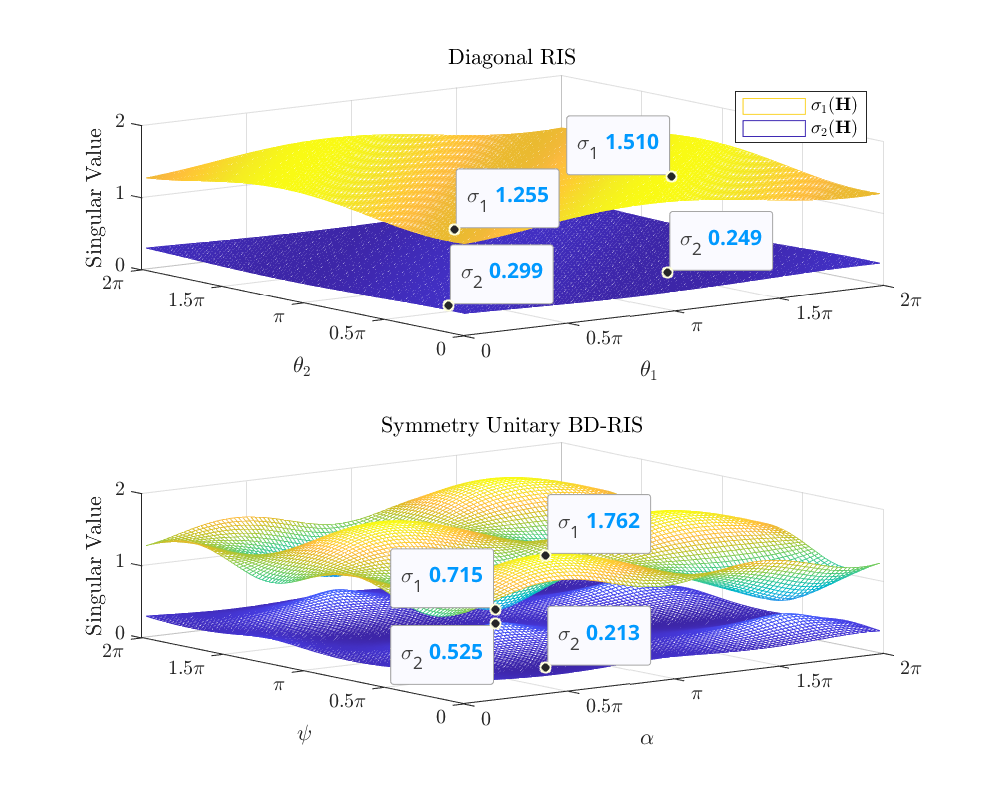
\includegraphics[width=\columnwidth]{../assets/simulation/pc_singular_trend.eps}
			\caption{$2 \times 2 \times 2$ singular value shaping by \gls{d}-\gls{ris} and symmetric fully-connected \gls{bd}-\gls{ris} when the direct channel is negligible. $\sigma_1(\mathbf{H})$ and $\sigma_2(\mathbf{H})$ refer to the most and least dominant singular values, respectively.
				Their maximum and minimum are marked explicitly on the plot.}
			\label{fg:shaping_potential}
		\end{figure}
		With an exhaustive grid search over $(\theta_1, \theta_2)$ and $(\alpha, \psi)$, Fig.~\ref{fg:shaping_potential} shows the achievable singular values of a specific channel realization
		\begin{equation*}
			\begin{split}
				\mathbf{H}_\mathrm{B} & =
				\begin{bmatrix}
					-0.2059 + 0.5914 \jmath & -0.0909 + 0.5861 \jmath \\
					0.4131 + 0.2651 \jmath  & -0.1960 + 0.4650 \jmath
				\end{bmatrix},
				\\
				\mathbf{H}_\mathrm{F} & =
				\begin{bmatrix}
					-0.6362 + 0.1332 \jmath & -0.1572 + 1.5538 \jmath \\
					0.0196 + 0.4011 \jmath  & -0.3170 - 0.2303 \jmath
				\end{bmatrix}.
			\end{split}
		\end{equation*}
		In this example, both singular values can be manipulated up to\footnote{The percentage for manipulating $\sigma_n(\mathbf{H})$ is calculated by $\eta_n^+ = \frac{\max \sigma_n(\mathbf{H}) - \mathrm{avg} \sigma_n(\mathbf{H})}{\mathrm{avg} \sigma_n(\mathbf{H})} \times 100\%$ and  $\eta_n^- = \frac{\min \sigma_n(\mathbf{H}) - \mathrm{avg} \sigma_n(\mathbf{H})}{\mathrm{avg} \sigma_n(\mathbf{H})} \times 100\%$.} $\pm 9\%$ by \gls{d}-\gls{ris} and $\pm 42\%$ by symmetric fully-connected \gls{bd}-\gls{ris}.
		It is noteworthy that the former requires 2 circuit components and the latter requires 3.
	\end{example}

	Example~\ref{eg:shaping_potential} suggests that the physical interconnection of \gls{ris} elements, even if using symmetric circuit components, can create a ``cooperation effect'' that significantly enhances the dynamic range of channel singular values.
	This motivates the analytical and numerical channel shaping studies in Section~\ref{sc:shaping_analytical} and \ref{sc:shaping_numerical}, respectively.

	\begin{subsection}{Analytical Shaping Bounds}
		\label{sc:shaping_analytical}
		The main results of this subsection are presented in the following Propositions and Corollaries.
		\begin{proposition}[Degrees of freedom]
			\label{pp:dof}
			\gls{bd}-\gls{ris} may achieve a larger or smaller number of \gls{mimo} \gls{dof}\footnote{\gls{dof} refers to the maximum number of independent streams that can be transmitted in parallel over a \gls{mimo} channel. It is defined as $\mathrm{DoF}(\mathbf{H}) = \lim_{\rho \to \infty} \frac{\log \det(\mathbf{I} + \rho \mathbf{H} \mathbf{H}^\mathsf{H})}{\log \rho}$ where $\rho$ is the \gls{snr}.} than \gls{d}-\gls{ris}.
		\end{proposition}
		\begin{proof}
			Please refer to Appendix~\ref{ap:dof}.
		\end{proof}

		Proposition \ref{pp:dof} suggests that we can expect more parallel streams or less interference when shaping the channel with \gls{bd}-\gls{ris}.
		We now take a step further to examine the limits of redistributing channel singular values under specific channel conditions.

		\begin{proposition}[Rank-deficient channel]
			\label{pp:rd}
			If the minimum rank of backward and forward channels is $k$ ($k \le N$),
			then for \gls{d}-\gls{ris} or \gls{bd}-\gls{ris} of arbitrary number of elements, the $n$-th singular value of the equivalent channel is bounded above and below respectively by
			\begin{subequations}
				\label{iq:sv_rd}
				\begin{align}
					\sigma_n(\mathbf{H}) & \le \sigma_{n-k}(\mathbf{T}), &  & \text{if } n > k, \label{iq:sv_rd_max}          \\
					\sigma_n(\mathbf{H}) & \ge \sigma_n(\mathbf{T}),     &  & \text{if } n < N - k + 1, \label{iq:sv_rd_min}
				\end{align}
			\end{subequations}
			where $\mathbf{T}$ is arbitrary auxiliary matrix satisfying
			\begin{equation}
				\label{eq:auxiliary_rd}
				\mathbf{T} \mathbf{T}^\mathsf{H} =
				\begin{cases}
					\mathbf{H}_\mathrm{D} (\mathbf{I} - \mathbf{V}_\mathrm{F} \mathbf{V}_\mathrm{F}^\mathsf{H}) \mathbf{H}_\mathrm{D}^\mathsf{H}, & \text{if } \rank(\mathbf{H}_\mathrm{F}) = k, \\
					\mathbf{H}_\mathrm{D}^\mathsf{H} (\mathbf{I} - \mathbf{U}_\mathrm{B} \mathbf{U}_\mathrm{B}^\mathsf{H}) \mathbf{H}_\mathrm{D}, & \text{if } \rank(\mathbf{H}_\mathrm{B}) = k,
				\end{cases}
			\end{equation}
			and $\mathbf{V}_\mathrm{F}$ and $\mathbf{U}_\mathrm{B}$ are any right and left singular matrices of $\mathbf{H}_\mathrm{F}$ and $\mathbf{H}_\mathrm{B}$, respectively.
		\end{proposition}
		\begin{proof}
			Please refer to Appendix~\ref{ap:rank_deficient}.
		\end{proof}

		Inequality \eqref{iq:sv_rd_max} states that
		if $\mathbf{H}_\mathrm{B}$ and $\mathbf{H}_\mathrm{F}$ are at least rank $k$, then
		with a \gls{d}-\gls{ris} or \gls{bd}-\gls{ris} of sufficiently large $N_\mathrm{S}$,
		the $n$-th singular value of $\mathbf{H}$ can be enlarged to the $(n-k)$-th singular value of $\mathbf{T}$, or suppressed to the $n$-th singular value of $\mathbf{T}$.
		Moreover, the first $k$ channel singular values are unbounded above\footnote{The energy conservation law $\sum_{n=1}^N \sigma_n^2(\mathbf{H}) \le 1$ still has to be respected in all cases. This constraint is omitted in context for brevity.} while the last $k$ channel singular values can be suppressed to zero.
		A special case is Corollary \ref{co:los} for \gls{los} channel\footnote{A similar eigenvalue result has been derived for \gls{d}-\gls{ris} only \cite{Semmler2023}.}.


		\begin{corollary}[\gls{los} channel]
			\label{co:los}
			If at least one of backward and forward channels is \gls{los}, then a \gls{d}-\gls{ris} or \gls{bd}-\gls{ris} can at most enlarge the $n$-th ($n \ge 2$) channel singular value to the $(n-1)$-th singular value of $\mathbf{T}$, or suppress the $n$-th channel singular value to the $n$-th singular value of $\mathbf{T}$.
			That is,
			\begin{equation}
				\label{iq:sv_los}
				\sigma_1(\mathbf{H}) \ge \sigma_1(\mathbf{T}) \ge {\sigma_2(\mathbf{H})} \ge \ldots \ge \sigma_{N-1}(\mathbf{T}) \ge {\sigma_N(\mathbf{H})} \ge \sigma_N(\mathbf{T}).
			\end{equation}
		\end{corollary}

		\begin{proof}
			This is a direct result of \eqref{iq:sv_rd} with $k = 1$.
		\end{proof}

		We emphasize that Proposition \ref{pp:rd} and Corollary \ref{co:los} apply to both \gls{d}- and \gls{bd}-\gls{ris} configurations regardless of the status of the direct channel.
		Out of $2N$ bounds in \eqref{iq:sv_rd} or \eqref{iq:sv_los}, $N$ of them can be \emph{simultaneously} tight as $N_\mathrm{S} \to \infty$, namely, when the direct channel becomes negligible\footnote{Negligible direct channel refers to the case where the power of the signal arriving at the receiver through the direct path is negligible compared to that through the scattering of \gls{ris}, i.e., $\mathbf{H} \approx \sum_g \mathbf{H}_g$. This can result from a very large number of \gls{ris} elements (as discussed in Proposition~\ref{pp:rd}) or physical obstacles in the propagation path (as discussed in Proposition~\ref{pp:nd}).}.
		For a finite $N_\mathrm{S}$, the \gls{ris} may prioritize a subset of those by aligning the corresponding modes, and we will later show by simulation that \gls{bd}-\gls{ris} outperforms \gls{d}-\gls{ris} on this purpose.
		Proposition \ref{pp:rd} provides a reference on the selection of $N_\mathrm{S}$ in low-multipath application scenarios.
		Next, we shift the focus to another popular \gls{ris} deployment scenario where the direct channel is blocked.


		\begin{proposition}[Negligible direct channel]
			\label{pp:nd}
			If the direct channel is negligible, then a fully-connected \gls{bd}-\gls{ris} can manipulate the channel singular values up to
			\begin{equation}
				\sv(\mathbf{H}) = \sv(\mathbf{BF}),
			\end{equation}
			where $\mathbf{B}$ and $\mathbf{F}$ are arbitrary matrices with $\sv(\mathbf{B})=\sv(\mathbf{H}_\mathrm{B})$ and $\sv(\mathbf{F})=\sv(\mathbf{H}_\mathrm{F})$.
		\end{proposition}

		\begin{proof}
			Please refer to Appendix~\ref{ap:nd}.
		\end{proof}

		Proposition \ref{pp:nd} says that if the direct channel is negligible and the \gls{bd}-\gls{ris} is fully-connected, the only singular value bounds on the equivalent channel are those on the product of unitary-transformed backward and forward channels.
		It is \emph{not necessarily} an asymptotic result and does \emph{not} depend on any relationship between $N_\mathrm{R}$, $N_\mathrm{S}$, and $N_\mathrm{T}$.
		Its importance lies in the fact that our initial channel shaping question can be recast as a linear algebra question: \emph{How the singular values of matrix product are bounded by the singular values of its individual factors?}
		The question is partially answered in Corollaries \ref{co:nd_sv_prod_subset}--\ref{co:nd_sv_indl} over definition\footnote{This is equivalent to padding zero blocks at the end of $\mathbf{H}, \mathbf{H}_\mathrm{B}, \mathbf{H}_\mathrm{F}$ to make square matrices of dimension $\bar{N}$.} $\bar{N} = \max(N_\mathrm{T},N_\mathrm{S},N_\mathrm{R})$ and $\sigma_n(\mathbf{H})=\sigma_n(\mathbf{H}_\mathrm{F})=\sigma_n(\mathbf{H}_\mathrm{B})=0, \ \forall n \in [\bar{N}] \setminus [N]$.
		The results are by no means complete and interested readers are referred to \cite[Chapter 16, 24]{Hogben2013} and \cite[Chapter 3]{Horn1994} for more information.


		\begin{corollary}[Product of subset of singular values]
			\label{co:nd_sv_prod_subset}
			If the direct channel is negligible,
			then the product of subset of singular values of $\mathbf{H}$ is bounded from above by those of $\mathbf{H}_\mathrm{B}$ and $\mathbf{H}_\mathrm{F}$, that is,
			\begin{equation}
				\label{iq:horn}
				\prod_{k \in {K}} \sigma_k(\mathbf{H}) \le \prod_{i \in {I}} \sigma_i(\mathbf{H}_\mathrm{B}) \prod_{j \in {J}} \sigma_j(\mathbf{H}_\mathrm{F}),
			\end{equation}
			for all admissible triples $(I, J, K) \in T_r^{\bar{N}}$ with $r < \bar{N}$, where
			\begin{equation*}
				\begin{split}
					T_r^{\bar{N}} \triangleq \Bigl\{(I, J, K) \in U_r^{\bar{N}} \bigm\vert & \forall p < r, \ \forall (F, G, H) \in T_p^r,                                              \\
																							& \sum_{f \in F} i_f + \sum_{g \in G} j_g \le \sum_{h \in H} k_h + \frac{p(p+1)}{2} \Bigr\},
				\end{split}
			\end{equation*}
			\begin{equation*}
				U_r^{\bar{N}} \triangleq \Bigl\{(I, J, K) \subseteq [\bar{N}]^3 \bigm\vert \sum_{i \in I} i + \sum_{j \in J} j = \sum_{k \in K} k + \frac{r(r+1)}{2}\Bigr\}.
			\end{equation*}
		\end{corollary}

		\begin{proof}
			Please refer to \cite[Theorem~8]{Fulton2000}.
		\end{proof}

		Inequality \eqref{iq:horn}, also recognized as a variation of Horn's inequality \cite{Bhatia2001}, is one of the most comprehensive result over Proposition \ref{pp:nd}.
		However, the number of admissible triples increases exponentially\footnote{For example, the number of inequalities described by \eqref{iq:horn} grows from 12 to 2062 when $N_\mathrm{S}$ increases from 3 to 7.} with $N_\mathrm{S}$ despite some resulting bounds can be redundant.
		We will shortly see \eqref{iq:horn} can also induce lower bounds on channel singular values.
		Those facts render the shaping limit analysis non-trivial for large-scale \gls{ris}-aided \gls{mimo} systems.
		Below we showcase some useful bounds therein.

		\begin{corollary}[Product of some largest or smallest singular values]
			\label{co:nd_sv_prod_tail}
			If the direct channel is negligible,
			then the product of the first (resp. last\footnote{The lower bounds coincide at zero when $N \ne N$ (i.e., $N_\mathrm{T} = N_\mathrm{S} = N_\mathrm{R}$ being false).}) $k$ singular values of $\mathbf{H}$ is bounded from above (resp. below) by those of $\mathbf{H}_\mathrm{B}$ and $\mathbf{H}_\mathrm{F}$, that is,
			\begin{subequations}
				\begin{align}
					\prod_{n=1}^k \sigma_n(\mathbf{H})                   & \le \prod_{n=1}^k \sigma_n(\mathbf{H}_\mathrm{B}) \sigma_n(\mathbf{H}_\mathrm{F}), \label{iq:sv_nd_prod_largest}                    \\
					\prod_{n=\bar{N}}^{\mathclap{\bar{N}-k+1}} \sigma_n(\mathbf{H}) & \ge \prod_{n=\bar{N}}^{\mathclap{\bar{N}-k+1}} \sigma_n(\mathbf{H}_\mathrm{B}) \sigma_n(\mathbf{H}_\mathrm{F}). \label{iq:sv_nd_prod_smallest}
				\end{align}
			\end{subequations}
		\end{corollary}

		\begin{proof}
			Please refer to Appendix~\ref{ap:nd_sv_prod_tail}.
		\end{proof}

		\begin{corollary}[Individual singular value]
			\label{co:nd_sv_indl}
			If the direct channel is negligible,
			then the $n$-th channel singular value can be manipulated up to
			\begin{equation}
				\label{iq:sv_nd_indl}
				\max_{\mathclap{i+j=n+N_\mathrm{S}}} \ \sigma_i(\mathbf{H}_\mathrm{B}) \sigma_j(\mathbf{H}_\mathrm{F}) \le \sigma_n(\mathbf{H}) \le \min_{\mathclap{i+j=n+1}} \ \sigma_i(\mathbf{H}_\mathrm{B}) \sigma_j(\mathbf{H}_\mathrm{F}),
			\end{equation}
			where $(i, j) \in [N_\mathrm{S}]^2$.
			The upper and lower bounds are attained respectively at
			\begin{subequations}
				\label{eq:ris_nd_sv_indl}
				\begin{align}
					\mathbf{\Theta}_{\textnormal{sv-}n\textnormal{-max}}^\textnormal{MIMO-ND} & = \mathbf{V}_\mathrm{B} \mathbf{P} \mathbf{U}_\mathrm{F}^\mathsf{H}, \label{eq:ris_nd_sv_indl_max} \\
					\mathbf{\Theta}_{\textnormal{sv-}n\textnormal{-min}}^\textnormal{MIMO-ND} & = \mathbf{V}_\mathrm{B} \mathbf{Q} \mathbf{U}_\mathrm{F}^\mathsf{H}, \label{eq:ris_nd_sv_indl_min}
				\end{align}
			\end{subequations}
			where $\mathbf{V}_\mathrm{B}, \mathbf{U}_\mathrm{F} \in \mathbb{U}^{N_\mathrm{S} \times N_\mathrm{S}}$ are any right and left singular matrices\footnote{
				\label{fn:svd_non_uniqueness}
				We highlight the non-uniqueness of $\mathbf{V}_\mathrm{B}$ and $\mathbf{U}_\mathrm{F}$. When a singular value has multiplicity $k$, the corresponding singular vectors can be any orthonormal basis of the $k$-dimensional subspace. Even if all singular values are distinct, the singular vectors of each can be scaled by a phase factor of choice.} of $\mathbf{H}_\mathrm{B}$ and $\mathbf{H}_\mathrm{F}$, respectively,
			and $\mathbf{P}$ and $\mathbf{Q}$ are arbitrary permutation matrices of dimension $N_\mathrm{S}$ satisfying:
			\begin{itemize}
				\item The $(i, j)$-th entry is $1$, where
					\begin{subnumcases}{(i, j) =}
						\ \underset{\mathclap{i+j=n+1}}{\arg\min} \ \sigma_i(\mathbf{H}_\mathrm{B}) \sigma_j(\mathbf{H}_\mathrm{F}) & for $\mathbf{P}$, \label{eq:idx_nd_sv_indl_max} \\
						\ \underset{\mathclap{i+j=n+N_\mathrm{S}}}{\arg\max} \ \sigma_i(\mathbf{H}_\mathrm{B}) \sigma_j(\mathbf{H}_\mathrm{F}) & for $\mathbf{Q}$, \label{eq:idx_nd_sv_indl_min}
					\end{subnumcases}
					and ties may be broken arbitrarily;
				\item After deleting the $i$-th row and $j$-th column, the resulting submatrix $\mathbf{Y}$ is arbitrary permutation matrix of dimension $N_\mathrm{S}-1$ satisfying
					\begin{subequations}
						\begin{alignat}{2}
							\sigma_{n{-}1}(\hat{\mathbf{\Sigma}}_{\mathrm{B}} \mathbf{Y} \hat{\mathbf{\Sigma}}_{\mathrm{F}}) & {\ge} \ \ \min_{\mathclap{i+j=n+1}} \ \sigma_i(\mathbf{H}_\mathrm{B}) \sigma_j(\mathbf{H}_\mathrm{F})            &  & \text{ for } \mathbf{P}, \label{eq:perm_nd_sv_indl_max} \\
							\sigma_{n{+}1}(\hat{\mathbf{\Sigma}}_{\mathrm{B}} \mathbf{Y} \hat{\mathbf{\Sigma}}_{\mathrm{F}}) & {\le} \ \ \max_{\mathclap{i+j=n+N_\mathrm{S}}} \ \sigma_i(\mathbf{H}_\mathrm{B}) \sigma_j(\mathbf{H}_\mathrm{F}) &  & \text{ for } \mathbf{Q}, \label{eq:perm_nd_sv_indl_min}
						\end{alignat}
					\end{subequations}
					where $\hat{\mathbf{\Sigma}}_{\mathrm{B}}$ and $\hat{\mathbf{\Sigma}}_{\mathrm{F}}$ are diagonal singular value matrices of $\mathbf{H}_\mathrm{B}$ and $\mathbf{H}_\mathrm{F}$ with both $i$-th row and $j$-th column deleted, respectively.
			\end{itemize}
		\end{corollary}

		\begin{proof}
			Please refer to Appendix~\ref{ap:nd_sv_indl}.
		\end{proof}

		Corollary \ref{co:nd_sv_indl} and Proposition \ref{pp:rd} both reveal the shaping limits of individual channel singular values.
		They are derived under different assumptions are not special cases of each other.
		Importantly, Corollary \ref{co:nd_sv_indl} establishes upper and lower bounds for \emph{each} channel singular value (c.f. first and last few in Proposition \ref{pp:rd}), applies to fully-connected \gls{bd}-\gls{ris} of arbitrary size, and provides a general solution structure.
		We emphasize that in \eqref{eq:ris_nd_sv_indl} the mode alignment is realized by $\mathbf{V}_\mathrm{B}$ and $\mathbf{U}_\mathrm{F}$ while the ordering is enabled by permutation matrices $\mathbf{P}$ and $\mathbf{Q}$, which are special cases of unitary $\mathbf{X}$ defined in \eqref{eq:ris_decompose}.
		Specially, the extreme channel singular values can be manipulated up to
		\begin{subequations}
			\label{iq:sv_nd_extreme}
			\begin{gather}
				\max_{\mathclap{i+j=N_\mathrm{S}+1}} \ \sigma_i(\mathbf{H}_\mathrm{B}) \sigma_j(\mathbf{H}_\mathrm{F}) {\le} \sigma_1(\mathbf{H}) {\le} \sigma_1(\mathbf{H}_\mathrm{B}) \sigma_1(\mathbf{H}_\mathrm{F}), \label{iq:sv_nd_largest} \\
				\min_{\mathclap{i+j=\bar{N}+1}} \ \sigma_i(\mathbf{H}_\mathrm{B}) \sigma_j(\mathbf{H}_\mathrm{F}) {\ge} \sigma_{\bar{N}}(\mathbf{H}) {\ge} \sigma_{\bar{N}}(\mathbf{H}_\mathrm{B}) \sigma_{\bar{N}}(\mathbf{H}_\mathrm{F}). \label{iq:sv_nd_smallest}
			\end{gather}
		\end{subequations}
		We notice that the right halves in \eqref{iq:sv_nd_largest} and \eqref{iq:sv_nd_smallest} are special cases of \eqref{iq:sv_nd_prod_largest} and \eqref{iq:sv_nd_prod_smallest} when $k=1$.

		\begin{example}[Bounds on $3 \times 3 \times 3$ shaping]
			\label{eg:shaping_bounds}
			Consider a $3 \times 3 \times 3$ setup with $\mathbf{H}_\mathrm{D} = \mathbf{0}$, $\mathbf{H}_\mathrm{B} = \diag(3, 2, 1)$, and $\mathbf{H}_\mathrm{F} = \diag(4, 0, 5)$.
			\begin{itemize}
				\item \gls{d}-\gls{ris}: It is evident that any \gls{d}-\gls{ris} can only achieve $\sv(\mathbf{H}) = [12, 5, 0]^\mathsf{T}$ due to limited branch matching and mode alignment capability.
				\item \gls{bd}-\gls{ris}: According to \eqref{iq:sv_nd_indl}, a fully-connected \gls{bd}-\gls{ris} can manipulate the singular values up to
					\begin{equation*}
						8 \le \sigma_1(\mathbf{H}) \le 15, \quad 4 \le \sigma_2(\mathbf{H}) \le 10, \quad 0 \le \sigma_3(\mathbf{H}) \le 0.
					\end{equation*}
					To attain the upper and lower bounds, $(i,j)$ in \eqref{eq:ris_nd_sv_indl_max} and \eqref{eq:ris_nd_sv_indl_min} takes $(1, 1)$ and $(2, 2)$ when $n=1$, and $(2, 1)$ and $(3, 2)$ when $n=2$, respectively.
			\end{itemize}
		\end{example}

		We conclude from Example \ref{eg:shaping_bounds} that a fully-connected \gls{bd}-\gls{ris} can widen the dynamic range of channel singular values by properly aligning and ordering the modes of $\mathbf{H}_\mathrm{B}$ and $\mathbf{H}_\mathrm{F}$.
		However, when the problem of interest is a function of multiple singular values, their individual bounds \eqref{iq:sv_nd_indl} may not be simultaneously tight.
		Some case studies are presented below.

		\begin{corollary}[Channel power gain]
			\label{co:nd_power}
			If the direct channel is negligible, then the channel power gain is bounded from above (resp. below) by the inner product of squared singular values of $\mathbf{H}_\mathrm{B}$ and $\mathbf{H}_\mathrm{F}$ when they are sorted similarly (resp. oppositely), that is,
			\begin{equation}
				\label{iq:power_nd}
				\sum_{n=1}^N \sigma_n^2(\mathbf{H}_\mathrm{B}) \sigma_{N_\mathrm{S}-n+1}^2(\mathbf{H}_\mathrm{F}) \le \lVert \mathbf{H} \rVert _\mathrm{F}^2 \le \sum_{n=1}^N \sigma_n^2(\mathbf{H}_\mathrm{B}) \sigma_n^2(\mathbf{H}_\mathrm{F}),
			\end{equation}
			whose\footnote{As a side note, we notice \cite{Fang1994} discussed a similar bound using extreme singular values $\max\bigl(\sigma_{N}(\mathbf{H}_\mathrm{B}) \lVert \mathbf{H}_\mathrm{F} \rVert _\mathrm{F}^2, \sigma_{N}(\mathbf{H}_\mathrm{F}) \lVert \mathbf{H}_\mathrm{B} \rVert _\mathrm{F}^2\bigr) \le \lVert \mathbf{H} \rVert _\mathrm{F}^2 \le \min\bigl(\sigma_1(\mathbf{H}_\mathrm{B}) \lVert \mathbf{H}_\mathrm{F} \rVert _\mathrm{F}^2, \sigma_1(\mathbf{H}_\mathrm{F}) \lVert \mathbf{H}_\mathrm{B} \rVert _\mathrm{F}^2\bigr)$. This is a looser version of \eqref{iq:power_nd} and cannot take equalities unless the extreme singular values are of multiplicity $N$.} upper and lower bounds are attained respectively at
			\begin{subequations}
				\begin{align}
					\mathbf{\Theta}_\textnormal{P-max}^\textnormal{MIMO-ND} & = \mathbf{V}_\mathrm{B} \mathbf{U}_\mathrm{F}^\mathsf{H}, \label{eq:ris_nd_power_max}            \\
					\mathbf{\Theta}_\textnormal{P-min}^\textnormal{MIMO-ND} & = \mathbf{V}_\mathrm{B} \mathbf{J} \mathbf{U}_\mathrm{F}^\mathsf{H} \label{eq:ris_nd_power_min},
				\end{align}
			\end{subequations}
			where $\mathbf{J}$ is the exchange (a.k.a. backward identity) matrix of dimension $N_\mathrm{S}$.
		\end{corollary}
		\begin{proof}
			Please refer to Appendix~\ref{ap:nd_power}.
		\end{proof}

		We notice that \eqref{eq:ris_nd_power_max} and \eqref{eq:ris_nd_power_min} are special cases of \eqref{eq:ris_nd_sv_indl_max} and \eqref{eq:ris_nd_sv_indl_min} with $\mathbf{P} = \mathbf{I}$ and $\mathbf{Q} = \mathbf{J}$, which also attain the right and left halves of \eqref{iq:sv_nd_extreme}, respectively.
		% TODO relay
		As a side note, when both $\mathbf{H}_\mathrm{B}$ and $\mathbf{H}_\mathrm{F}$ follow Rayleigh fading, the expectation of maximum channel power gain can be numerically evaluated as
		\begin{equation}
			\label{eq:power_nd_rayleigh}
			\begin{split}
				\mathbb{E}\bigl\{ \lVert \mathbf{H} \rVert _ \mathrm{F}^2 \bigr\} = \sum_{n=1}^N
				& \int_0^\infty x f_{\lambda_n^{\min(N_\mathrm{R},N_\mathrm{S})}}(x) d x         \\
				& \times \int_0^\infty y f_{\lambda_n^{\min(N_\mathrm{S},N_\mathrm{T})}}(y) d y,
			\end{split}
		\end{equation}
		where $\lambda_n^{K}$ is the $n$-th eigenvalue of the complex $K \times K$ Wishart matrix with probability density function $f_{\lambda_n^{K}}(\cdot)$ given by \cite[(51)]{Zanella2009}.
		\eqref{eq:power_nd_rayleigh} generalizes the \gls{siso} channel power gain aided by \gls{bd}-\gls{ris} \cite[(58)]{Shen2020a} to \gls{mimo} under double Rayleigh fading, but a closed-form expression seems nontrivial.
		The next corollary has been derived in \cite{Bartoli2023} independently from Proposition \ref{pp:nd} and we include it here for completeness of results.
		\begin{corollary}[Channel capacity at general \gls{snr}]
			\label{co:nd_capacity_snr_general}
			If the direct channel is negligible, then the \gls{bd}-\gls{ris} aided \gls{mimo} channel capacity is
			\begin{equation}
				\label{eq:capacity_nd}
				C^\textnormal{MIMO-ND} = \sum_{n=1}^N \log \left(1 + \frac{s_n \sigma_n^2(\mathbf{H}_\mathrm{B}) \sigma_n^2(\mathbf{H}_\mathrm{F})}{\eta}\right),
			\end{equation}
			where $\eta$ is the average noise power, $s_n = \mu - \frac{\eta}{\sigma_n^2(\mathbf{H}_\mathrm{B}) \sigma_n^2(\mathbf{H}_\mathrm{F})}$ is the power allocated to the $n$-th mode obtainable by the water-filling algorithm \cite{Clerckx2013}.
			The capacity-achieving \gls{bd}-\gls{ris} scattering matrix is
			\begin{equation}
				\label{eq:ris_nd_rate_max}
				\mathbf{\Theta}_\textnormal{R-max}^\textnormal{MIMO-ND} = \mathbf{V}_\mathrm{B} \mathbf{U}_\mathrm{F}^\mathsf{H}.
			\end{equation}
		\end{corollary}

		\begin{proof}
			Please refer to \cite[Appendix~A]{Bartoli2023}.
		\end{proof}

		Corollary \ref{co:nd_capacity_snr_general} also suggests that the power- and rate-optimal scattering matrices \eqref{eq:ris_nd_power_max} and \eqref{eq:ris_nd_rate_max} coincide with each other when the direct channel is negligible and the \gls{bd}-\gls{ris} is fully-connected.
		When either condition is not satisfied, active and passive beamforming are coupled and the rate-optimal solution involves alternating optimization.
		However, the power-optimal \gls{ris} still provides for a low-complexity decoupled solution.
		The details will be discussed in Section~\ref{sc:rate_pc}.

		\begin{corollary}[Channel capacity at extreme \gls{snr}]
			\label{co:nd_capacity_snr_extreme}
			If the direct channel is negligible, then the channel capacity when the \gls{snr} $\rho$ is very low and high are approximately bounded from above by
			\begin{subequations}
				\label{iq:capacity_nd_snr_extreme}
				\begin{align}
					C_{\rho_\downarrow} & \lessapprox \sigma_1^2(\mathbf{H}_\mathrm{B}) \sigma_1^2(\mathbf{H}_\mathrm{F}), \label{iq:capacity_nd_snr_low}                                           \\
					C_{\rho_\uparrow}   & \lessapprox N \log \frac{\rho}{N} + 2 \log \prod_{n=1}^N \sigma_n(\mathbf{H}_\mathrm{B}) \sigma_n(\mathbf{H}_\mathrm{F}). \label{iq:capacity_nd_snr_high}
				\end{align}
			\end{subequations}
		\end{corollary}

		\begin{proof}
			Please refer to Appendix~\ref{ap:nd_capacity}.
		\end{proof}

		The ergodic counterparts of \eqref{eq:capacity_nd} and \eqref{iq:capacity_nd_snr_extreme} when both $\mathbf{H}_\mathrm{B}$ and $\mathbf{H}_\mathrm{F}$ follow Rayleigh fading can be evaluated similarly to \eqref{eq:power_nd_rayleigh}.
		Proposition \ref{pp:dof}--\ref{pp:nd} and the resulting Corollaries provide a partial answer to the channel shaping question in terms of singular values and their functions.
		Extending the analysis to more general cases (e.g., non-negligible direct channel and arbitrary \gls{bd}-\gls{ris} group size) is non-trivial due to limited branch matching and mode alignment capabilities therein.
		A numerical solution will be discussed in Section~\ref{sc:shaping_numerical}.
	\end{subsection}

	\begin{subsection}{Numerical Shaping Solution}
		\label{sc:shaping_numerical}
		Consider a special class of channel shaping problem
		\begin{maxi!}
			{\scriptstyle{\mathbf{\Theta}}}{f\bigl(\sv(\mathbf{H})\bigr)}{\label{op:shaping}}{\label{ob:shaping}}
			\addConstraint{\mathbf{\Theta}_g^\mathsf{H} \mathbf{\Theta}_g=\mathbf{I},}{\quad \forall g,}{\label{cn:shaping_unitary}}
		\end{maxi!}
		where $f: \mathbb{R}^{N} \to \mathbb{R}$ is a symmetric gauge function (i.e., a norm invariant under sign change and argument permutation) \cite{Watson1992}.
		Examples of such $f$ include the Ky Fan $k$ norm, Schatten $p$ norm, $n$-th singular value, and channel power gain.
		Problem \eqref{op:shaping} is non-convex due to the unitary constraints \eqref{cn:shaping_unitary}.
		\begin{proposition}
			\label{pp:shaping}
			The sub-differential of \eqref{ob:shaping} with respect to \gls{bd}-\gls{ris} block $g$ is
			\begin{equation}
				\label{eq:shaping_subdiff}
				\partial_{\mathbf{\Theta}_g^*} f\bigl(\sv(\mathbf{H})\bigr) = \conv \bigl\{ \mathbf{H}_{\mathrm{B},g}^\mathsf{H} \mathbf{U} \mathbf{D} \mathbf{V}^\mathsf{H} \mathbf{H}_{\mathrm{F},g}^\mathsf{H} \bigr\},
			\end{equation}
			where $\mathbf{D} \in \mathbb{C}^{N_\mathrm{R} \times N_\mathrm{T}}$ is a rectangular diagonal matrix with $[\mathbf{D}]_{n,n} \in \partial_{\sigma_n(\mathbf{H})} f\bigl(\sv(\mathbf{H})\bigr)$, $\forall n \in [N]$, and $\mathbf{U}$, $\mathbf{V}$ are any left and right singular matrices of $\mathbf{H}$.
		\end{proposition}

		\begin{proof}
			Please refer to Appendix~\ref{ap:shaping}.
		\end{proof}

		With Proposition \ref{pp:shaping}, one can apply the \emph{relax-then-project} method \cite{Shen2020a,Fang2023} or \emph{non-geodesic\footnote{A geodesic is a curve representing the shortest path between two points in a Riemannian manifold, whose tangent vectors remain parallel when transporting along the curve.} \gls{rcg}} \cite{Li2023b,Li2023c,Zhou2023} to solve Problem \eqref{op:shaping}.
		The former solves unconstrained problem \eqref{ob:shaping} by quasi-Newton methods and projects the solution back to domain \eqref{cn:shaping_unitary} without guarantee of optimality.
		The latter generalizes the conjugate gradient methods to Riemannian manifolds and updates the solution by addition and retraction, which constitutes a zigzag path departing from and returning to the manifold.
		Next, we introduce a group-wise \emph{geodesic \gls{rcg}} method modified from \cite{Abrudan2008,Abrudan2009} that performs multiplicative updates along the geodesics on the Stiefel manifold for faster convergence.
		It is applicable to a wide range of \gls{bd}-\gls{ris} design problems where the objective $f$ is smooth or convex non-smooth\footnote{$f$ is not necessarily the symmetric gauge function \eqref{ob:shaping}.} and the only constraint is group-wise unitarity \eqref{cn:shaping_unitary}.
		The steps for updating $\mathbf{\Theta}_g$ at iteration $r$ are summarized below:
		\begin{enumerate}
			\item \emph{Compute the Euclidean (sub-)gradient at $\mathbf{\Theta}_g^{(r)}$:} The (sub-)gradient of $f$ with respect to $\mathbf{\Theta}_g$ in the Euclidean space is
			% \cite[(A.3.6)]{Fischer2005}
				\begin{equation}
					\label{eq:gradient_eucl}
					\nabla_{\mathrm{E},g}^{(r)} = 2 \frac{\partial f(\mathbf{\Theta}_g^{(r)})}{\partial \mathbf{\Theta}_g^*};
				\end{equation}
			\item \emph{Translate to the Riemannian (sub-)gradient at $\mathbf{\Theta}_g^{(r)}$:} At point $\mathbf{\Theta}_g^{(r)}$, the Riemannian (sub-)gradient gives the steepest ascent direction on the manifold. It lies in the tangent space of the manifold $\mathcal{T}_{\mathbf{\Theta}_g^{(r)}}\mathbb{U}^{L \times L} \triangleq \{\mathbf{M} \in \mathbb{C}^{L \times L} \mid \mathbf{M}^\mathsf{H} \mathbf{\Theta}_g^{(r)} + {\mathbf{\Theta}_g^{(r)\mathsf{H}}} \mathbf{M} = \mathbf{0}\}$ and is obtainable by projection:
				\begin{equation}
					\label{eq:gradient_riem}
					\nabla_{\mathrm{R},g}^{(r)} = \nabla_{\mathrm{E},g}^{(r)} - \mathbf{\Theta}_g^{(r)} {\nabla_{\mathrm{E},g}^{(r)\mathsf{H}}} \mathbf{\Theta}_g^{(r)};
				\end{equation}
			\item \emph{Translate to the Riemannian (sub-)gradient at the identity:} The Riemannian (sub-)gradient should be translated back to the identity for exploiting the Lie algebra\footnote{Lie algebra refers to the tangent space of the Lie group at the identity element. A Lie group is simultaneously a continuous group and a differentiable manifold. In this example, $\mathbb{U}^{L \times L}$ formulates a Lie group and the corresponding Lie algebra consists of skew-Hermitian matrices $\mathfrak{u}(L) \triangleq \mathcal{T}_{\mathbf{I}}\mathbb{U}^{L \times L} = \{\mathbf{M} \in \mathbb{C}^{L \times L} \mid \mathbf{M}^\mathsf{H} + \mathbf{M} = \mathbf{0}\}$.}:
				\begin{equation}
					\label{eq:gradient_riem_tran}
					\tilde{\nabla}_{\mathrm{R},g}^{(r)} = \nabla_{\mathrm{R},g}^{(r)} \mathbf{\Theta}_g^{(r)\mathsf{H}} = \nabla_{\mathrm{E},g}^{(r)} \mathbf{\Theta}_g^{(r)\mathsf{H}} - \mathbf{\Theta}_g^{(r)} {\nabla_{\mathrm{E},g}^{(r)\mathsf{H}}}.
					% $\mathcal{O}(2 L^3)$
				\end{equation}
			\item \emph{Determine the conjugate direction:} The conjugate direction is obtained over the Riemannian (sub-)gradient and previous direction as
				\begin{equation}
					\label{eq:conjugate_dirn_geod}
					{\mathbf{D}}_g^{(r)} = \tilde{\nabla}_{\mathrm{R},g}^{(r)} + {\gamma}_g^{(r)} {\mathbf{D}}_g^{(r-1)},
				\end{equation}
				where $\gamma_g^{(r)}$ is the parameter that deviates the conjugate direction from the tangent space for accelerated convergence. A popular choice is the Polak-Ribi\`{e}re formula \cite{Hager2006}
				\begin{equation}
					\label{eq:conjugate_parm_geod}
					{\gamma}_g^{(r)} = \frac{\tr\bigl((\tilde{\nabla}_{\mathrm{R},g}^{(r)} - \tilde{\nabla}_{\mathrm{R},g}^{(r-1)}) {\tilde{\nabla}_{\mathrm{R},g}^{(r)\mathsf{H}}}\bigr)}{\tr\bigl(\tilde{\nabla}_{\mathrm{R},g}^{(r-1)} {\tilde{\nabla}_{\mathrm{R},g}^{(r-1)\mathsf{H}}}\bigr)}. % $\mathcal{O}(2 N_\mathrm{S}^3 + N_\mathrm{S}^2 + 2 N_\mathrm{S})$
				\end{equation}
			\item \emph{Evaluate the geodesic at the identity:} The geodesic emanating from the identity with velocity $\mathbf{D} \in \mathfrak{u}(L)$ is described by
				\begin{equation}
					\label{eq:geodesic_iden}
					\mathbf{G}_\mathbf{I}(\mu) = \exp(\mu \mathbf{D}),
				\end{equation}
				where $\exp(\mathbf{A}) = \sum_{k=0}^\infty (\mathbf{A}^k/k!)$ is the matrix exponential and $\mu$ is the step size (i.e., magnitude of the tangent vector).
			\item \emph{Translate to the geodesic at $\mathbf{\Theta}_g^{(r)}$:} The geodesic emanating from $\mathbf{\Theta}_g^{(r)}$ terminates at $\mathbf{\Theta}_g^{(r+1)}$ by multiplicative updates
				\begin{equation}
					\label{eq:geodesic_tran}
					\mathbf{\Theta}_g^{(r+1)} = \mathbf{G}_{\mathbf{\Theta}_g^{(r)}}(\mu) = \mathbf{G}_\mathbf{I}(\mu) \mathbf{\Theta}_g^{(r)} = \exp(\mu \mathbf{D}_g^{(r)}) \mathbf{\Theta}_g^{(r)},
				\end{equation}
				where $\mu$ is the step size refinable\footnote{To double the step size, one can simply square the rotation matrix instead of recomputing the matrix exponential, that is, $\exp^2(\mu \mathbf{D}_g^{(r)}) = \exp(2 \mu \mathbf{D}_g^{(r)})$.} by the Armijo rule \cite{Armijo1966}.
		\end{enumerate}

		\begin{algorithm}[!t]
			\caption{Group-wise geodesic \gls{rcg}}
			\label{ag:rcg}
			\begin{algorithmic}[1]
				\Require $f(\mathbf{\Theta})$, $G$
				\Ensure $\mathbf{\Theta}^\star$
				\Initialize {$r \gets 0$, $\mathbf{\Theta}^{(0)}$}
				\Repeat
				\For {$g \gets 1$ to $G$}
				\State $\nabla_{\mathrm{E},g}^{(r)} \gets$ \eqref{eq:gradient_eucl}, $\tilde{\nabla}_{\mathrm{R},g}^{(r)} \gets$ \eqref{eq:gradient_riem_tran}
				\State $\tilde{\gamma}_g^{(r)} \gets$ \eqref{eq:conjugate_parm_geod}, $\mathbf{D}_g^{(r)} \gets$ \eqref{eq:conjugate_dirn_geod}
				\If {$\Re\bigl\{\tr({\mathbf{D}_g^{(r)\mathsf{H}}} \tilde{\nabla}_{\mathrm{R},g}^{(r)})\bigr\} < 0$} \Comment{Not ascent}
				\State $\mathbf{D}_g^{(r)} \gets \tilde{\nabla}_{\mathrm{R},g}^{(r)}$
				\EndIf
				\State $\mu \gets 0.1$
				\State $\mathbf{G}_{\mathbf{\Theta}_g^{(r)}}(\mu) \gets$ \eqref{eq:geodesic_tran}
				\While {$ f\bigl(\mathbf{G}_{\mathbf{\Theta}_g^{(r)}}(2\mu)\bigr) - f(\mathbf{\Theta}_g^{(r)}) \ge \mu \cdot \frac{\tr(\mathbf{D}_g^{(r)} {\mathbf{D}_g^{(r)\mathsf{H}}})}{2}$}\label{ln:armijo_start}
				\State $\mu \gets 2 \mu$
				\EndWhile
				\While {$f\bigl(\mathbf{G}_{\mathbf{\Theta}_g^{(r)}}(\mu)\bigr) - f(\mathbf{\Theta}_g^{(r)}) < \frac{\mu}{2} \cdot \frac{\tr(\mathbf{D}_g^{(r)} {\mathbf{D}_g^{(r)\mathsf{H}}})}{2}$}
				\State $\mu \gets \mu / 2$
				\EndWhile \label{ln:armijo_end}
				\State $\mathbf{\Theta}_g^{(r+1)} \gets$ \eqref{eq:geodesic_tran}
				\EndFor
				\State $r \gets r+1$
				\Until $\lvert f(\mathbf{\Theta}^{(r)}) - f(\mathbf{\Theta}^{(r-1)}) \rvert / f(\mathbf{\Theta}^{(r-1)}) \le \epsilon$
			\end{algorithmic}
		\end{algorithm}

		Algorithm~\ref{ag:rcg} summarizes the introduced group-wise geodesic \gls{rcg} method.
		Compared to the non-geodesic approach, it leverages Lie algebra to replace the add-then-retract update with a multiplicative update \eqref{eq:geodesic_tran} along the geodesics of the Stiefel manifold.
		This appropriate parameter space leads to faster convergence and easier step size tuning.
		Convergence to a local optimum is still guaranteed if not initialized at a stationary point.
		The group-wise updates can be performed in parallel to facilitate large-scale \gls{bd}-\gls{ris} design problems.
		One can also directly operate on $\mathbf{\Theta}$ and pinching (i.e., keeping the main block diagonal and nulling others) relevant expressions to accelerate the algorithm for a large $G$.

		We now analyze the computational complexity of solving singular value shaping problem \eqref{op:shaping} by Algorithm~\ref{ag:rcg}.
		To update each \gls{bd}-\gls{ris} group, \gls{svd} of $\mathbf{H}$ requires $\mathcal{O}(N N_\mathrm{T} N_\mathrm{R})$, Euclidean sub-gradient \eqref{eq:shaping_subdiff} requires $\mathcal{O}\bigl(L N (N_\mathrm{T}+N_\mathrm{R}+L) \bigr)$, Riemannian sub-gradient translation \eqref{eq:gradient_riem_tran} requires $\mathcal{O}(L^3)$, deviation parameter \eqref{eq:conjugate_parm_geod} and conjugate direction \eqref{eq:conjugate_dirn_geod} together require $\mathcal{O}(L^2)$, and matrix exponential \eqref{eq:geodesic_tran} requires $\mathcal{O}(L^3)$ operations \cite{Moler2003}.
		The overall complexity is thus $\mathcal{O}\bigl(I_\text{RCG} G \bigl(N N_\mathrm{T} N_\mathrm{R} + L N (N_\mathrm{T}+N_\mathrm{R}+L) + I_\text{BLS} L^3\bigr)\bigr)$, where $I_\text{RCG}$ and $I_\text{BLS}$ are the number of iterations for geodesic \gls{rcg} and backtracking line search (i.e., line \ref{ln:armijo_start}--\ref{ln:armijo_end} of Algorithm \ref{ag:rcg}), respectively.
		That is, $\mathcal{O}_\mathrm{D}\bigl(N_\mathrm{S}\bigr)$ for \gls{d}-\gls{ris} and $\mathcal{O}_\mathrm{BD}\bigl(N_\mathrm{S}^3\bigr)$ for fully-connected \gls{bd}-\gls{ris}.
		% That is, $\mathcal{O}_\mathrm{D}\bigl(I_\text{RCG} N_\mathrm{S} \bigl(N N_\mathrm{T} N_\mathrm{R} + N (N_\mathrm{T}+N_\mathrm{R}) + I_\text{BLS}\bigr)\bigr)$ for \gls{d}-\gls{ris} and $\mathcal{O}_\mathrm{BD}\bigl(I_\text{RCG} \bigl(N N_\mathrm{T} N_\mathrm{R} + N_\mathrm{S} N (N_\mathrm{T}+N_\mathrm{R}+N_\mathrm{S}) + I_\text{BLS} N_\mathrm{S}^3\bigr)\bigr)$ for fully-connected \gls{bd}-\gls{ris}.

		To validate Algorithm~\ref{ag:rcg} and quantify the shaping capability of \gls{bd}-\gls{ris}, we characterize the achievable singular value region of \gls{bd}-\gls{ris}-aided \gls{mimo} channel by considering the Pareto optimization problem
		\begin{maxi!}
			{\scriptstyle{\mathbf{\Theta}}}{\sum_{n=1}^N \rho_n \sigma_n(\mathbf{H})}{\label{op:pareto}}{\label{ob:pareto}}
			\addConstraint{\mathbf{\Theta}_g^\mathsf{H} \mathbf{\Theta}_g=\mathbf{I},}{\quad \forall g,}{\label{cn:pareto_unitary}}
		\end{maxi!}
		where $\rho_n \ge 0$ is the weight associated with the $n$-th channel singular value.
		Varying those weights help to characterize the Pareto frontier of singular values that encloses the achievable region.
		While the objective \eqref{ob:pareto} does not suggest any meaningful performance metric (e.g., capacity or power gain), there exists an implicit relation since stronger channel shaping capability translates to better wireless performance.
		Problem \eqref{op:pareto} also generalizes the \gls{dof} problem in Proposition \ref{pp:dof} and the individual singular value shaping problem in Corollary \ref{co:nd_sv_indl} and Proposition \ref{pp:rd}.
		It can be solved optimally by Algorithm~\ref{ag:rcg} with $\mathbf{D}_{[n,n]} = \rho_n$ in \eqref{eq:shaping_subdiff}.
	\end{subsection}
\end{section}


	\begin{section}{Rate Maximization}
		\label{sc:rate}
		In this section, we first solve rate maximization problem for \gls{bd}-\gls{ris}-aided \gls{mimo} point-to-point and interference channels optimally by joint beamforming design, and then exploit channel shaping for a low-complexity two-stage solution.

		\begin{subsection}{MIMO Point-to-Point Channel}
			\label{sc:rate_pc}
			The achievable rate maximization problem for \gls{bd}-\gls{ris}-aided \gls{mimo} point-to-point channel is formulated as
			\begin{maxi!}
				{\scriptstyle{\mathbf{W},\mathbf{\Theta}}}{R = \log \det \biggl(\mathbf{I} + \frac{\mathbf{W}^\mathsf{H}\mathbf{H}^\mathsf{H}\mathbf{H}\mathbf{W}}{\eta}\biggr)}{\label{op:rate}}{\label{ob:rate}}
				\addConstraint{\lVert \mathbf{W} \rVert _\mathrm{F}^2}{\le P}
				\addConstraint{\mathbf{\Theta}_g^\mathsf{H} \mathbf{\Theta}_g}{=\mathbf{I}, \quad \forall g,\label{cn:rate_unitary}}
			\end{maxi!}
			where $\mathbf{W}$ is the transmit precoder, $R$ is the achievable rate, $\eta$ is the average noise power, and $P$ is maximum average transmit power.
			Problem \eqref{op:rate} is non-convex due to the block-unitary constraint \eqref{cn:rate_unitary} and the coupling between variables.
			Two approaches are proposed to solve it optimally or efficiently.
			% We propose a local-optimal approach based on \gls{ao} and a low-complexity approach based on channel shaping.

			\begin{subsubsection}{Alternating Optimization}
				This approach updates $\mathbf{\Theta}$ and $\mathbf{W}$ iteratively until convergence.
				For a given $\mathbf{W}$, the passive beamforming subproblem is
				\begin{maxi!}
					{\scriptstyle{\mathbf{\Theta}}}{\log \det \biggl(\mathbf{I} + \frac{\mathbf{H} \mathbf{Q} \mathbf{H}^\mathsf{H}}{\eta}\biggr)}{\label{op:rate_ris}}{\label{ob:rate_ris}}
					\addConstraint{\mathbf{\Theta}_g^\mathsf{H} \mathbf{\Theta}_g=\mathbf{I}, \quad \forall g,}{}{}
				\end{maxi!}
				where $\mathbf{Q} \triangleq \mathbf{W} \mathbf{W}^\mathsf{H}$ is the transmit covariance matrix.
				Problem \eqref{op:rate_ris} can be solved optimally by Algorithm \ref{ag:rcg} with the partial derivative given in Lemma \ref{lm:rate}.
				\begin{lemma}
					\label{lm:rate}
					The partial derivative of \eqref{ob:rate_ris} with respect to \gls{bd}-\gls{ris} block $g$ is
					\begin{equation}
						\label{eq:gradient_eucl_rate}
						\frac{\partial R}{\partial \mathbf{\Theta}_g^*} = \frac{1}{\eta} \mathbf{H}_{\mathrm{B},g}^\mathsf{H} \biggl(\mathbf{I} + \frac{\mathbf{H}\mathbf{Q}\mathbf{H}^\mathsf{H}}{\eta}\biggr)^{-1} \mathbf{H} \mathbf{Q} \mathbf{H}_{\mathrm{F},g}^\mathsf{H}.
					\end{equation}
				\end{lemma}

				\begin{proof}
					Please refer to Appendix~\ref{ap:rate}.
				\end{proof}
				For a given $\mathbf{\Theta}$, the optimal transmit precoder is given by eigenmode transmission \cite{Clerckx2013}
				\begin{equation}
					\label{eq:precoder_rate}
					\mathbf{W}^\star = \mathbf{V} {\diag(\mathbf{s}^\star)}^{1/2},
				\end{equation}
				where $\mathbf{V}$ is the right singular matrix of $\mathbf{H}$ and $\mathbf{s}^\star$ is the optimal water-filling power allocation \cite{Clerckx2013}.
				The \gls{ao} algorithm is guaranteed to converge to local-optimal points of problem \eqref{op:rate} since each subproblem is solved optimally and the objective is bounded above.
				The computational complexity of solving subproblem \eqref{op:rate_ris} by geodesic \gls{rcg} is $\mathcal{O}\bigl(I_\text{RCG} G (NL^2 + L N_\mathrm{T} N_\mathrm{R} + N_\mathrm{T}^2 N_\mathrm{R} + N_\mathrm{T} N_\mathrm{R}^2 + N_\mathrm{R}^3 + I_\text{BLS} L^3)\bigr)$.
				On the other hand, the complexity of solving active beamforming subproblem by \eqref{eq:precoder_rate} is $\mathcal{O}\bigl(N N_\mathrm{T} N_\mathrm{R}\bigr)$.
				The overall complexity is thus $\mathcal{O}\bigl(I_\text{AO}\bigl(I_\text{RCG} G (NL^2 + L N_\mathrm{T} N_\mathrm{R} + N_\mathrm{T}^2 N_\mathrm{R} + N_\mathrm{T} N_\mathrm{R}^2 + N_\mathrm{R}^3 + I_\text{BLS} L^3) + N N_\mathrm{T} N_\mathrm{R}\bigr)\bigr)$, where $I_\text{AO}$ is the number of iterations for \gls{ao}.
				That is, $\mathcal{O}_\mathrm{D}\bigl(N_\mathrm{S}\bigr)$ for \gls{d}-\gls{ris} and $\mathcal{O}_\mathrm{BD}\bigl(N_\mathrm{S}^3\bigr)$ for fully-connected \gls{bd}-\gls{ris}.
				% That is, $\mathcal{O}_\mathrm{D}\bigl(I_\text{AO}\bigl(I_\text{RCG} N_\mathrm{S} (N + N_\mathrm{T} N_\mathrm{R} + N_\mathrm{T}^2 N_\mathrm{R} + N_\mathrm{T} N_\mathrm{R}^2 + N_\mathrm{R}^3 + I_\text{BLS}) + N N_\mathrm{T} N_\mathrm{R}\bigr)\bigr)$ for \gls{d}-\gls{ris} and $\mathcal{O}_\mathrm{BD}\bigl(I_\text{AO}\bigl(I_\text{RCG} (NN_\mathrm{S}^2 + N_\mathrm{S} N_\mathrm{T} N_\mathrm{R} + N_\mathrm{T}^2 N_\mathrm{R} + N_\mathrm{T} N_\mathrm{R}^2 + N_\mathrm{R}^3 + I_\text{BLS} N_\mathrm{S}^3) + N N_\mathrm{T} N_\mathrm{R}\bigr)\bigr)$ for fully-connected \gls{bd}-\gls{ris}.
			\end{subsubsection}

			\begin{subsubsection}{Low-Complexity Solution}
				\label{sc:rate_pc_lc}
				To reduce the computational complexity, we suboptimally decouple the beamforming design by first shape the channel by \gls{ris} for maximum power gain and then optimize the active beamforming.
				The channel power gain maximization problem is formulated as\footnote{Problem \eqref{op:power} has been studied in \gls{siso} \cite{Shen2020a} and \gls{miso} equivalents \cite{Santamaria2023,Fang2023,Nerini2023,Nerini2023b} where only one mode is available. Generalizing those to \gls{mimo} is non-trivial due to trade-off between modes.}
				\begin{maxi!}
					{\scriptstyle{\mathbf{\Theta}}}{\lVert \mathbf{H}_\mathrm{D} + \mathbf{H}_\mathrm{B} \mathbf{\Theta} \mathbf{H}_\mathrm{F} \rVert _\mathrm{F}^2}{\label{op:power}}{\label{ob:power}}
					\addConstraint{\mathbf{\Theta}_g^\mathsf{H} \mathbf{\Theta}_g=\mathbf{I}, \quad \forall g.}{\label{cn:power_unitary}}{}
				\end{maxi!}
				Inspired by \cite{Nie2017}, we propose a closed-form iterative solution that converges to a stationary point of Problem \eqref{op:power}.
				The idea is to approximate the quadratic objective \eqref{ob:power} successively by Taylor expansion and solve each subproblem by group-wise \gls{svd}.

				\begin{proposition}
					\label{pp:power}
					Starting from any feasible $\mathbf{\Theta}^{(0)}$, the sequence
					\begin{equation}
						\label{eq:ris_power}
						\mathbf{\Theta}_g^{(r+1)} = \mathbf{U}_g^{(r)} \mathbf{V}_g^{(r)}, \quad \forall g
					\end{equation}
					leads to a convergence of the objective function \eqref{ob:power} towards a stationary point,\footnote{However, \eqref{eq:ris_power} might not converge to a single solution point due to the non-uniqueness of \gls{svd}, especially when $\mathbf{M}_g$ is rank-deficient.}
					% Multiple solutions may yield similar objective function convergence behavior.}
					where $\mathbf{U}_g^{(r)}$ and $\mathbf{V}_g^{(r)}$ are any left and right singular matrices of\footnote{We notice that the orthogonal projection of $\mathbf{M}_g$ onto the Stiefel manifold $\pi(\mathbf{M}_g) = {\arg\min}_{\mathbf{X}_g \in \mathbb{U}^{L \times L}} \lVert \mathbf{M}_g - \mathbf{X}_g \rVert _\mathrm{F} = \mathbf{U}_g \mathbf{V}_g$ coincides with $\mathbf{\Theta}_g$.} % \cite{Manton2002}
					\begin{equation}
						\label{eq:auxiliary_power}
						\mathbf{M}_g^{(r)} = \mathbf{H}_{\mathrm{B},g}^\mathsf{H} \Bigl(\mathbf{H}_\mathrm{D} + \mathbf{H}_\mathrm{B} \diag\bigl(\mathbf{\Theta}_{[1:g-1]}^{(r+1)},\mathbf{\Theta}_{[g:G]}^{(r)}\bigr) \mathbf{H}_\mathrm{F}\Bigr) \mathbf{H}_{\mathrm{F},g}^\mathsf{H}.
					\end{equation}
				\end{proposition}

				\begin{proof}
					Please refer to Appendix~\ref{ap:power}.
				\end{proof}

				To update each \gls{bd}-\gls{ris} group, matrix multiplication \eqref{eq:auxiliary_power} requires $\mathcal{O}\bigl(N_\mathrm{T} N_\mathrm{R} + NL^2+N_\mathrm{T} N_\mathrm{R} L\bigr)$ operations and its \gls{svd} requires $\mathcal{O}(L^3)$ operations.
				The overall complexity is thus $\mathcal{O}\bigl(I_\text{SAA} G \bigl(N_\mathrm{T} N_\mathrm{R} + NL^2+N_\mathrm{T} N_\mathrm{R} L + L^3\bigr)\bigr)$, where $I_\text{SAA}$ is the number iterations for successive affine approximation.
				That is, $\mathcal{O}_\mathrm{D}\bigl(N_\mathrm{S}\bigr)$ for \gls{d}-\gls{ris} and $\mathcal{O}_\mathrm{BD}\bigl(N_\mathrm{S}^3\bigr)$ for fully-connected \gls{bd}-\gls{ris}.
				% That is, $\mathcal{O}_\mathrm{D}\bigl(I_\text{SAA} N_\mathrm{S} \bigl(N_\mathrm{T} N_\mathrm{R} + N+N_\mathrm{T} N_\mathrm{R}\bigr)\bigr)$ for \gls{d}-\gls{ris} and $\mathcal{O}_\mathrm{BD}\bigl(I_\text{SAA} \bigl(N_\mathrm{T} N_\mathrm{R} + NN_\mathrm{S}^2+N_\mathrm{T} N_\mathrm{R} N_\mathrm{S} + N_\mathrm{S}^3\bigr)\bigr)$ for fully-connected \gls{bd}-\gls{ris}.
				% It is noteworthy that the computational complexity can be further reduced
				For the latter, the computational complexity can be further reduced:
				\begin{itemize}
					\item \emph{Negligible direct channel:} The optimal solution to \eqref{op:power} has been solved in closed form by \eqref{eq:ris_nd_power_max}.
					\item \emph{Non-negligible direct channel:} In terms of maximizing the inner product $\langle \mathbf{H}_\mathrm{D}, \mathbf{H}_\mathrm{B} \mathbf{\Theta} \mathbf{H}_\mathrm{F} \rangle$, \eqref{op:power} is reminiscent of the weighted orthogonal Procrustes problem \cite{Gower2004}
					\begin{mini!}
						{\scriptstyle{\mathbf{\Theta}}}{\lVert \mathbf{H}_\mathrm{D} - \mathbf{H}_\mathrm{B} \mathbf{\Theta} \mathbf{H}_\mathrm{F} \rVert _\mathrm{F}^2}{\label{op:procrustes_wt}}{}
						\addConstraint{\mathbf{\Theta}^\mathsf{H} \mathbf{\Theta}=\mathbf{I},}{\label{cn:procrustes_wt}}{}
					\end{mini!}
					which still has no trivial solution.
					One \emph{lossy} transformation \cite{Bell2003} shifts $\mathbf{\Theta}$ to sides of the product by Moore-Penrose inverse, formulating standard orthogonal Procrustes problems
					\begin{mini!}
						{\scriptstyle{\mathbf{\Theta}}}{\lVert \mathbf{H}_\mathrm{B}^\dagger \mathbf{H}_\mathrm{D} - \mathbf{\Theta} \mathbf{H}_\mathrm{F} \rVert _\mathrm{F}^2 \text{ or } \lVert \mathbf{H}_\mathrm{D} \mathbf{H}_\mathrm{F}^\dagger - \mathbf{H}_\mathrm{B} \mathbf{\Theta} \rVert _\mathrm{F}^2}{\label{op:procrustes}}{}
						\addConstraint{\mathbf{\Theta}^\mathsf{H} \mathbf{\Theta}=\mathbf{I},}{}{}
					\end{mini!}
					with optimal solutions \cite[(6.4.1)]{Golub2013}
					\begin{equation}
						\label{eq:ris_procrustes}
						\mathbf{\Theta}_\textnormal{P-max-approx}^\textnormal{MIMO-HD} = \mathbf{U} \mathbf{V}^\mathsf{H},
					\end{equation}
					where $\mathbf{U}$ and $\mathbf{V}$ are respectively any left and right singular matrices of $\mathbf{H}_\mathrm{B}^\dagger \mathbf{H}_\mathrm{D} \mathbf{H}_\mathrm{F}^\mathsf{H}$ or $\mathbf{H}_\mathrm{B}^\mathsf{H} \mathbf{H}_\mathrm{D} \mathbf{H}_\mathrm{F}^\dagger$.
				\end{itemize}

				Although \eqref{eq:ris_nd_power_max} and \eqref{eq:ris_procrustes} are of similar form, the latter is neither optimal nor a generalization of the former due to the lossy transformation.
				We will show in Section \ref{sc:simulation} that $\mathbf{\Theta}_\textnormal{P-max-approx}^\textnormal{MIMO-HD}$ is very close to optimal especially for a large $N_\mathrm{S}$.
				Once the channel is shaped by \eqref{eq:ris_power} or \eqref{eq:ris_nd_power_max} or \eqref{eq:ris_procrustes}, the active beamforming is retrieved by \eqref{eq:precoder_rate}.
				This two-stage solution avoids outer iterations and efficiently handles (or avoids) inner iterations.
			\end{subsubsection}
		\end{subsection}

		\begin{subsection}{MIMO Interference Channel}
			On top of \eqref{eq:channel_interference}, the achievable rate of transmission $k$ is
			\begin{equation}
				R_k = \log \det \biggl(\mathbf{I} + \mathbf{W}_k {\mathbf{H}^{(kj)\mathsf{H}}} \mathbf{Q}_k^{-1} {\mathbf{H}^{(kj)}} \mathbf{W}_k\biggr),
			\end{equation}
			where $\mathbf{W}_k$ is the precoder at transmitter $k$ and $\mathbf{Q}_k = \sum_{j \ne k} {\mathbf{H}^{(kj)}} \mathbf{W}_j \mathbf{W}_j^\mathsf{H} {\mathbf{H}^{(kj)\mathsf{H}}} + \eta \mathbf{I}$ is the interference-plus-noise covariance matrix at receiver $k$.
			The weighted sum-rate maximization problem for \gls{bd}-\gls{ris}-aided \gls{mimo} interference channel is formulated as
			\begin{maxi!}
				{\scriptstyle{\mathbf{\Theta}, \{\mathbf{W}_k\}_{k \in [K]}}}{\sum_{k=1}^K \rho_k R_k}{\label{op:wsr}}{\label{ob:wsr}}
				\addConstraint{\mathbf{\Theta}_g^\mathsf{H} \mathbf{\Theta}_g=\mathbf{I}, \quad \forall g}{}{}
				\addConstraint{\lVert \mathbf{W}_k \rVert _\mathrm{F}^2 \le P_k. \quad \forall k}{}{}
			\end{maxi!}
			where $\rho_k \ge 0$ is the weight associated with transmission $k$.
			This non-convex problem can be solved by extending both solutions covered in Section \ref{sc:rate_pc} as detailed below.

			\begin{subsubsection}{Alternating Optimization}
				This approach updates $\mathbf{\Theta}$ and $\{\mathbf{W}_k\}_{k \in [K]}$ iteratively until convergence.
				For a given precoder set, the passive beamforming subproblem is
				\begin{maxi!}
					{\scriptstyle{\mathbf{\Theta}}}{\sum_{k=1}^K \rho_k R_k}{\label{op:wsr_ris}}{\label{ob:wsr_ris}}
					\addConstraint{\mathbf{\Theta}_g^\mathsf{H} \mathbf{\Theta}_g=\mathbf{I}, \quad \forall g,}{}{}
				\end{maxi!}
				which can be solved optimally by Algorithm \ref{ag:rcg} with the partial derivative given in Lemma \ref{lm:wsr}.

				\begin{lemma}
					\label{lm:wsr}
					The partial derivative of \eqref{ob:wsr_ris} with respect to \gls{bd}-\gls{ris} block $g$ is
					\begin{equation}
						\label{eq:gradient_eucl_wsr}
						\begin{split}
							\frac{\partial \rho_k R_k}{\partial \mathbf{\Theta}_g^*} = \sum_{k=1}^K & \rho_k {\mathbf{H}^{(k)\mathsf{H}}_{\mathrm{B},g}} \mathbf{Q}_k^{-1} {\mathbf{H}^{(kk)}} \mathbf{W}_k \mathbf{E}_k \mathbf{W}_k^\mathsf{H} \\
							& \times \bigl({\mathbf{H}_{\mathrm{F},g}^{(k)\mathsf{H}}} - {\mathbf{H}^{(kk)\mathsf{H}}} \mathbf{Q}_k^{-1} \sum_{j \ne k} {\mathbf{H}^{(kj)}} \mathbf{W}_j \mathbf{W}_j^\mathsf{H} {\mathbf{H}^{(j)\mathsf{H}}_{\mathrm{F},g}}\bigr),
						\end{split}
					\end{equation}
					where $\mathbf{E}_k = \bigl(\mathbf{I} + {\mathbf{W}_k^\mathsf{H}} {\mathbf{H}^{(kk)\mathsf{H}}} \mathbf{Q}_k {\mathbf{H}^{(kk)}} \mathbf{W}_k\bigr)^{-1}$ is the error matrix of receiver $k$.
				\end{lemma}

				\begin{proof}
					Please refer to Appendix~\ref{ap:wsr}.
				\end{proof}

				For a given $\mathbf{\Theta}$, problem \eqref{op:wsr} reduces to conventional precoding design for interference channel.
				A closed-form iterative solution based on mutual information-\gls{mmse} relationship has been proposed in \cite{Shin2012,Negro2010} and we summarize the steps as follows.
				At iteration $r$, the \gls{mmse} combiner at receiver $k$ is
				\begin{equation}
					\begin{split}
						\mathbf{G}_k^{(r)} &= {\mathbf{W}_k^{(r-1)\mathsf{H}}} {\mathbf{H}^{(kk)\mathsf{H}}} \\
						& \quad \times \bigl(\mathbf{Q}_k^{(r-1)} + {\mathbf{H}^{(kk)}} \mathbf{W}_k^{(r-1)} {\mathbf{W}_k^{(r-1)\mathsf{H}}} {\mathbf{H}^{(kk)\mathsf{H}}}\bigr)^{-1},
					\end{split}
				\end{equation}
				the corresponding error matrix is
				\begin{equation}
					\mathbf{E}_k^{(r)} = \bigl(\mathbf{I} + {\mathbf{W}_k^{(r-1)\mathsf{H}}} {\mathbf{H}^{(kk)\mathsf{H}}} \mathbf{Q}_k^{(r-1)} {\mathbf{H}^{(kk)}} \mathbf{W}_k^{(r-1)}\bigr)^{-1},
				\end{equation}
				and the optimal precoder at transmitter $k$ is given by
				\begin{equation}
					\label{eq:precoder_wsr}
					\begin{split}
						\mathbf{W}_k^{(r)} & = \Bigl(\sum_{j=1}^K {\mathbf{H}^{(jk)\mathsf{H}}} {\mathbf{G}_j^{(r)\mathsf{H}}} \mathbf{\Omega}_k^{(r)} \mathbf{G}_j^{(r)} \mathbf{H}^{(jk)} + \lambda_k^{(r)} \mathbf{I} \Bigr)^{-1} \\
						& \quad \times {\mathbf{H}^{(kk)\mathsf{H}}} {\mathbf{G}_j^{(r)\mathsf{H}}} \mathbf{\Omega}_k^{(r)},
					\end{split}
				\end{equation}
				where $\mathbf{\Omega}_k^{(r)} = \rho_k {\mathbf{E}_k^{(r)-1}}$ is the mean-square error weight and $\lambda_k^{(r)}$ is the Lagrange multiplier retrievable by bisection \cite{Shin2012} or in closed form \cite{Negro2010}
				\begin{equation}
					\lambda_k^{(r)} = \frac{\mathrm{tr}\bigl(\eta \mathbf{\Omega}_k^{(r)} \mathbf{G}_k^{(r)}{\mathbf{G}_k^{(r)\mathsf{H}}} + \sum_{j=1}^K (\mathbf{Z}_{kj}^{(r)} - \mathbf{Z}_{jk}^{(r)}) \bigr)}{P_k},
					% \lambda_k^{(r)} = \frac{\mathrm{tr}\bigl(\eta \mathbf{\Omega}_k^{(r)} \mathbf{G}_k^{(r)}{\mathbf{G}_k^{(r)\mathsf{H}}} + \sum_j \mathbf{\Omega}_k^{(r)}\mathbf{T}_{kj}^{(r)} {\mathbf{T}_{kj}^{(r)\mathsf{H}}} - \mathbf{\Omega}_j^{(r)}\mathbf{T}_{jk}^{(r)} {\mathbf{T}_{jk}^{(r)\mathsf{H}}} \bigr)}{P_k},
				\end{equation}
				where $\mathbf{Z}_{kj}^{(r)} = \mathbf{\Omega}_k^{(r)}\mathbf{T}_{kj}^{(r)} {\mathbf{T}_{kj}^{(r)\mathsf{H}}}$ and $\mathbf{T}_{kj}^{(r)} = \mathbf{G}_k^{(r)} {\mathbf{H}^{(kj)}} \mathbf{W}_j^{(r)}$.

				The computational complexity of solving subproblem \eqref{op:wsr_ris} by geodesic \gls{rcg} is $\mathcal{O}\bigl(I_\text{RCG} G (N_\mathrm{T} d^2 + N_\mathrm{T}^2 d + N_\mathrm{T}^2 N_\mathrm{R} + N_\mathrm{T} N_\mathrm{R}^2 + K (N_\mathrm{T} N_\mathrm{R} d + N_\mathrm{T} N_\mathrm{R} L) + I_\text{BLS}L^3)\bigr)$.
				That is, $\mathcal{O}_\mathrm{D}\bigl(N_\mathrm{S}\bigr)$ for \gls{d}-\gls{ris} and $\mathcal{O}_\mathrm{BD}\bigl(N_\mathrm{S}^3\bigr)$ for fully-connected \gls{bd}-\gls{ris}.
			\end{subsubsection}

			\begin{subsubsection}{Low-Complexity Solution}
				Similar to Section \ref{sc:rate_pc_lc}, we suboptimally decouple the beamforming design by first shape the channel by \gls{ris} for minimum leakage interference and then optimize the active beamforming.
				The leakage interference minimization problem is formulated as
				\begin{mini!}
					{\scriptstyle{\mathbf{\Theta}}}{I = \sum_{k=1}^K \sum_{j \ne k} \left\lVert {\mathbf{H}}^{(kj)}_\mathrm{D} + {\mathbf{H}}^{(k)}_\mathrm{B} \mathbf{\Theta} {\mathbf{H}}^{(j)}_\mathrm{F} \right\rVert _{\mathrm{F}}^2}{\label{op:interference}}{\label{ob:interference}}
					\addConstraint{\mathbf{\Theta}_g^\mathsf{H} \mathbf{\Theta}_g=\mathbf{I}, \quad \forall g,}{}{}
				\end{mini!}
				which can be solved iteratively in closed form.

				\begin{proposition}
					\label{pp:interference}
					Starting from any feasible $\mathbf{\Theta}^{(0)}$, the sequence
					\begin{equation}
						\mathbf{\Theta}_g^{(r+1)} = \mathbf{U}_g^{(r)} \mathbf{V}_g^{(r)}, \quad \forall g
						\label{eq:scatter_leakage}
					\end{equation}
					converges to a stationary point of \eqref{op:interference}, where $\mathbf{U}_g^{(r)}$ and $\mathbf{V}_g^{(r)}$ are any left and right singular matrices of
					\begin{equation}
						\mathbf{M}_g^{(r)} = \sum_{k=1}^K \sum_{j \ne k} \bigl(\mathbf{B}_g^{(k)} \mathbf{\Theta}_g^{(r)} \mathbf{H}^{(j)}_{\mathrm{F},g} - {\mathbf{H}^{(k)\mathsf{H}}_{\mathrm{B},g}} {\mathbf{D}^{(kj)(r)}_{g}}\bigr) {\mathbf{H}^{(j)\mathsf{H}}_{\mathrm{F},g}},
					\end{equation}
					where $\mathbf{B}_g^{(k)} = \lambda_1\bigl({\mathbf{H}^{(k)\mathsf{H}}_{\mathrm{B},g}} \mathbf{H}^{(k)}_{\mathrm{B},g}\bigr) \mathbf{I} - {\mathbf{H}^{(k)\mathsf{H}}_{\mathrm{B},g}} \mathbf{H}^{(k)}_{\mathrm{B},g}$ and ${\mathbf{D}^{(kj)(r)}_{g}} = \mathbf{H}^{(kj)}_\mathrm{D} + \sum_{g'<g} {\mathbf{H}_{\mathrm{B},g'}^{(k)\mathsf{H}}} \mathbf{\Theta}_{g'}^{(r+1)} \mathbf{H}_{\mathrm{F},g'}^{(k)} + \sum_{g'>g} {\mathbf{H}_{\mathrm{B},g'}^{(k)\mathsf{H}}} \mathbf{\Theta}_{g'}^{(r)} \mathbf{H}_{\mathrm{F},g'}^{(k)}.$
				\end{proposition}
				\begin{proof}
					Please refer to Appendix~\ref{ap:interference}.
				\end{proof}
			\end{subsubsection}
			Once the channel is shaped by \eqref{eq:scatter_leakage}, the active beamforming is retrieved iteratively by \eqref{eq:precoder_wsr}.
			This Two-stage solution avoids outer iterations and efficiently handles inner iterations.
		\end{subsection}

			% \begin{subsection}{Leakage Interference Minimization}
			% 	Leakage interference refers to the sum of all interference terms in \gls{ic}.
			% 	Assume all transmitter sends $N_\mathrm{E} \le N \triangleq \min(N_\mathrm{T}, N_\mathrm{R})$ data streams to its intended receiver.
			% 	The leakage interference minimization problem is formulated with respect to all transmit precoders, all receiver combiners, and the scattering matrix as
			% 	\begin{mini!}
			% 		{\scriptstyle{\mathbf{\Theta}, \{\mathbf{G}_k\}, \{\mathbf{W}_k\}_{k \in [K]}}}{\mathop{\sum\sum}_{j \neq k} \left\lVert \mathbf{G}_k (\mathbf{H}^{(kj)}_\mathrm{D} + \mathbf{H}^{(k)}_\mathrm{B} \mathbf{\Theta} \mathbf{H}^{(j)}_{\mathrm{F}}) \mathbf{W}_j \right\rVert _{\mathrm{F}}^2}{\label{op:leakage}}{}
			% 		\addConstraint{\mathbf{\Theta}_g^\mathsf{H} \mathbf{\Theta}_g=\mathbf{I}, \quad}{\forall g}{\label{co:scatter}}
			% 		\addConstraint{\mathbf{G}_k \mathbf{G}_k^\mathsf{H}=\mathbf{I}, \quad}{\forall k}{\label{co:combiner}}
			% 		\addConstraint{\mathbf{W}_j^\mathsf{H} \mathbf{W}_j=\mathbf{I}, \quad}{\forall j,}{\label{co:precoder}}
			% 	\end{mini!}
			% 	where $\mathbf{G}_k \in \mathbb{C}^{N_\mathrm{D} \times N_\mathrm{R}}$ is the combiner at receiver $k$ and $\mathbf{W}_j \in \mathbb{C}^{N_\mathrm{T} \times N_\mathrm{D}}$ is the precoder at transmitter $j$.
			% 	It is worth noting that $\mathbf{\Theta}_g$ is a square unitary matrix and $\mathbf{\Theta}_g^\mathsf{H} \mathbf{\Theta}_g=\mathbf{I}$ is equivalent to $\mathbf{\Theta}_g \mathbf{\Theta}_g^\mathsf{H}=\mathbf{I}$, while $\mathbf{G}_k$ and $\mathbf{W}_j$ may be respectively ``fat'' and ``tall'' rectangular semi-unitary matrices such that \eqref{co:combiner} and \eqref{co:precoder} are required.
			% 	The non-convex problem can be solved iteratively by the \gls{bcd} method detailed below.

			% 	\begin{subsubsection}{Combiner and Precoder Design}
			% 		For a given $\mathbf{\Theta}$, problem \eqref{op:leakage} reduces to conventional linear beamforming problem, for which an iterative algorithm alternating between the original and reciprocal networks is proposed in \cite{Gomadam2011,Clerckx2013}.
			% 		At iteration $r$, the combiner at receiver $k$ is updated as
			% 		\begin{equation}
			% 			\mathbf{G}_k^{(r)} = {\mathbf{U}_{k,N}^{(r-1)}}^\mathsf{H},
			% 			\label{eq:combiner_leakage}
			% 		\end{equation}
			% 		where $\mathbf{U}_{k,N}^{(r-1)}$ is the eigenvectors corresponding to $N$ smallest eigenvalues of the interference covariance matrix $\mathbf{Q}_k^{(r-1)} = \sum_{j \ne k} {\mathbf{H}^{(kj)}} \mathbf{W}_j^{(r-1)} {\mathbf{W}_j^{(r-1)}}^\mathsf{H} {\mathbf{H}^{(kj)\mathsf{H}}}$.
			% 		The precoder at transmitter $j$ is updated as
			% 		\begin{equation}
			% 			\mathbf{W}_j^{(r)} = \bar{\mathbf{U}}_{j,N}^{(r)},
			% 			\label{eq:precoder_leakage}
			% 		\end{equation}
			% 		where $\bar{\mathbf{U}}_{j,N}^{(r)}$ corresponds $\bar{\mathbf{Q}}_j^{(r)} = \sum_{k \ne j} {\mathbf{H}^{(kj)\mathsf{H}}} {\mathbf{G}_k^{(r)\mathsf{H}}} \mathbf{G}_k^{(r)} {\mathbf{H}^{(kj)}}$ in the reciprocal network.
			% 	\end{subsubsection}

			% 	\begin{subsubsection}{Scattering Matrix Design}
			% 		Once $\{\mathbf{G}_k\}$ and $\{\mathbf{W}_j\}$ are determined, we define $\bar{\mathbf{H}}^{(kj)}_\mathrm{D} \triangleq \mathbf{G}_k \mathbf{H}^{(kj)}_\mathrm{D} \mathbf{W}_j$, $\bar{\mathbf{H}}^{(k)}_\mathrm{B} \triangleq \mathbf{G}_k \mathbf{H}^{(k)}_\mathrm{B}$, and $\bar{\mathbf{H}}^{(j)}_\mathrm{F} \triangleq \mathbf{H}^{(j)}_\mathrm{F} \mathbf{W}_j$.
			% 		The \gls{bd}-\gls{ris} subproblem boils down to
			% 		\begin{mini!}
			% 			{\scriptstyle{\mathbf{\Theta}}}{\mathop{\sum\sum}_{j \neq k} \left\lVert (\bar{\mathbf{H}}^{(kj)}_\mathrm{D} + \bar{\mathbf{H}}^{(k)}_\mathrm{B} \mathbf{\Theta} \bar{\mathbf{H}}^{(j)}_\mathrm{F}) \right\rVert _{\mathrm{F}}^2}{\label{op:ic_interference_ris}}{}
			% 			\addConstraint{\mathbf{\Theta}_g^\mathsf{H} \mathbf{\Theta}_g=\mathbf{I}, \quad \forall g,}{}{}
			% 		\end{mini!}
			% 		which can be viewed as a channel shaping problem on $\bar{\mathbf{H}}^{(kj)}_\mathrm{D}$, $\bar{\mathbf{H}}^{(k)}_\mathrm{B}$, and $\bar{\mathbf{H}}^{(j)}_\mathrm{F}$.

			% 		\begin{proposition}
			% 			Start from any $\mathbf{\Theta}^{(0)}$, the sequence
			% 			\begin{equation}
			% 				\mathbf{\Theta}_g^{(r+1)} = \mathbf{U}_g^{(r)} \mathbf{V}_g^{(r)}, \quad \forall g
			% 				\label{eq:scatter_leakage}
			% 			\end{equation}
			% 			converges to a stationary point of \eqref{op:ic_interference_ris}, where $\mathbf{U}_g^{(r)}$ and $\mathbf{V}_g^{(r)}$ are left and right singular matrix of
			% 			\begin{equation}
			% 				\mathbf{M}_g^{(r)} = \mathop{\sum\sum}_{j \neq k} \bigl(\mathbf{B}_{k,g} \mathbf{\Theta}_g^{(r)} \mathbf{H}^{(j)}_{\mathrm{F},g} - {\mathbf{H}^{(k)\mathsf{H}}_{\mathrm{B},g}} {\mathbf{D}^{(kj)}_{g}}^{(r)}\bigr) {\mathbf{H}^{(j)\mathsf{H}}_{\mathrm{F},g}},
			% 			\end{equation}
			% 			where $\mathbf{B}_{k,g} = \lambda_1\bigl({\mathbf{H}^{(k)\mathsf{H}}_{\mathrm{B},g}} \mathbf{H}^{(k)}_{\mathrm{B},g}\bigr) \mathbf{I} - {\mathbf{H}^{(k)\mathsf{H}}_{\mathrm{B},g}} \mathbf{H}^{(k)}_{\mathrm{B},g}$ and
			% 			\begin{equation}
			% 				{\mathbf{D}^{(kj)}_{g}}^{(r)} = \mathbf{H}^{(kj)}_\mathrm{D} + \sum_{g'<g} {\mathbf{H}_{k,g'}^\mathrm{B}}^\mathsf{H} \mathbf{\Theta}_{g'}^{(r+1)} \mathbf{H}_{k,g'}^\mathrm{F} + \sum_{g'>g} {\mathbf{H}_{k,g'}^\mathrm{B}}^\mathsf{H} \mathbf{\Theta}_{g'}^{(r)} \mathbf{H}_{k,g'}^\mathrm{F}.
			% 			\end{equation}
			% 		\end{proposition}
			% 		\begin{proof}
			% 			The proof is similar to Appendix~\ref{ap:power} and omitted here.
			% 		\end{proof}
			% 	\end{subsubsection}

			% 	Problem \eqref{op:leakage} can be solved iteratively by \eqref{eq:combiner_leakage}, \eqref{eq:precoder_leakage}, and \eqref{eq:scatter_leakage}.
			% 	Convergence to local-optimal points is guaranteed since each subproblem is solved optimally and the objective is bounded above.

			% \end{subsection}

			% \begin{subsection}{Weighted Sum-Rate Maximization}
			% 	Finally, we consider weighted sum-rate maximization in \gls{mimo}-\gls{ic} by joint active beamforming design at the transmitters and passive beamforming design at the \gls{ris}.
			% 	The achievable rate of transmission $k$ is given by
			% 	\begin{equation}
			% 		R_k = \log \det \biggl(\mathbf{I} + \mathbf{W}_k {\mathbf{H}^{(kj)\mathsf{H}}} \mathbf{Q}_k^{-1} {\mathbf{H}^{(kj)}} \mathbf{W}_k\biggr),
			% 	\end{equation}
			% 	where $\mathbf{Q}_k$ is the interference-plus-noise covariance matrix at receiver $k$
			% 	\begin{equation}
			% 		\mathbf{Q}_k = \sum_{j \ne k} {\mathbf{H}^{(kj)}} \mathbf{W}_j \mathbf{W}_j^\mathsf{H} {\mathbf{H}^{(kj)\mathsf{H}}} + \eta \mathbf{I},
			% 	\end{equation}
			% 	and $\eta$ is the average noise power.
			% 	The optimization problem is formulated as
			% 	\begin{maxi!}
			% 		{\scriptstyle{\mathbf{\Theta}, \{\mathbf{W}_k\}_{k \in [K]}}}{\sum_k \rho_k R_k}{\label{op:ic_rate}}{\label{ob:ic_rate}}
			% 		\addConstraint{\mathbf{\Theta}_g^\mathsf{H} \mathbf{\Theta}_g=\mathbf{I}, \quad \forall g}{}{}
			% 		\addConstraint{\lVert \mathbf{W}_k \rVert _\mathrm{F}^2 \le P_k. \quad \forall k}{}{}
			% 	\end{maxi!}
			% 	where $\rho_k$ is the weight that denotes the priority of transmission $k$.
			% 	The problem is non-convex and can be solved by the \gls{ao} method detailed below.

			% 	\begin{subsubsection}{Precoder Design}
			% 		For a given $\mathbf{\Theta}$, \eqref{op:ic_rate} reduces to conventional linear beamforming problem, for which a closed-form iterative solution has been proposed in \cite{Negro2010} based on mutual information-\gls{mmse} relationship \cite{Guo2005}.
			% 		We restate the steps as follows.

			% 		At iteration $r$, the \gls{mmse} combiner at receiver $k$ is
			% 		\begin{equation}
			% 			\mathbf{G}_k^{(r)} = {\mathbf{W}_k^{(r-1)\mathsf{H}}} {\mathbf{H}^{(kk)\mathsf{H}}} \bigl(\mathbf{Q}_k^{(r-1)} + {\mathbf{H}^{(kk)}} \mathbf{W}_k^{(r-1)} {\mathbf{W}_k^{(r-1)\mathsf{H}}} {\mathbf{H}^{(kk)\mathsf{H}}}\bigr)^{-1},
			% 		\end{equation}
			% 		the corresponding error matrix is
			% 		\begin{equation}
			% 			\mathbf{E}_k^{(r)} = \bigl(\mathbf{I} + {\mathbf{W}_k^{(r-1)\mathsf{H}}} {\mathbf{H}^{(kk)\mathsf{H}}} \mathbf{Q}_k^{(r-1)} {\mathbf{H}^{(kk)}} \mathbf{W}_k^{(r-1)}\bigr)^{-1},
			% 		\end{equation}
			% 		the \gls{mse} weight is
			% 		\begin{equation}
			% 			\mathbf{\Omega}_k^{(r)} = \rho_k {\mathbf{E}_k^{(r)}}^{-1},
			% 		\end{equation}
			% 		the Lagrange multiplier is
			% 		\begin{equation}
			% 			\lambda_k^{(r)} = \frac{\mathrm{tr}\bigl(\eta \mathbf{\Omega}_k^{(r)} \mathbf{G}_k^{(r)}{\mathbf{G}_k^{(r)\mathsf{H}}} + \sum_j \mathbf{\Omega}_k^{(r)}\mathbf{T}_{kj}^{(r)} {\mathbf{T}_{kj}^{(r)\mathsf{H}}} - \mathbf{\Omega}_j^{(r)}\mathbf{T}_{jk}^{(r)} {\mathbf{T}_{jk}^{(r)}}^\mathsf{H} \bigr)}{P_k},
			% 		\end{equation}
			% 		where $\mathbf{T}_{kj}^{(r)} = \mathbf{G}_k^{(r)} {\mathbf{H}^{(kj)}} \mathbf{W}_j^{(r)}$.
			% 		The optimal precoder at transmitter $k$ is given by
			% 		\begin{equation}
			% 			\mathbf{W}_k^{(r)} = \Bigl(\sum_j {\mathbf{H}^{(jk)\mathsf{H}}} {\mathbf{G}_j^{(r)\mathsf{H}}} \mathbf{\Omega}_k^{(r)} \mathbf{G}_j^{(r)} \mathbf{H}^{(jk)} + \lambda_k^{(r)} \mathbf{I} \Bigr)^{-1} {\mathbf{H}^{(kk)\mathsf{H}}} {\mathbf{G}_j^{(r)\mathsf{H}}} \mathbf{\Omega}_k^{(r)}.
			% 		\end{equation}
			% 	\end{subsubsection}

			% 	\begin{subsubsection}{Scattering Matrix Design}
			% 		Once $\{\mathbf{W}_k\}$ is determined, the complex derivative of \eqref{ob:ic_rate} with respect to \gls{ris} block $g$ is
			% 		\begin{equation}
			% 			\frac{\partial \rho_k R_k}{\partial \mathbf{\Theta}_g^*} = \sum_k \rho_k {\mathbf{H}^{(k)\mathsf{H}}_{\mathrm{B},g}} \mathbf{Q}_k^{-1} {\mathbf{H}^{(kk)}} \mathbf{W}_k \mathbf{E}_k \mathbf{W}_k^\mathsf{H} \bigl({\mathbf{H}_{\mathrm{F},g}^{(k)\mathsf{H}}} - {\mathbf{H}^{(kk)\mathsf{H}}} \mathbf{Q}_k^{-1} \sum_{j \ne k} {\mathbf{H}^{(kj)}} \mathbf{W}_j \mathbf{W}_j^\mathsf{H} {\mathbf{H}^{(j)\mathsf{H}}_{\mathrm{F},g}}\bigr).
			% 			\label{eq:ic_rate_gradient_ris}
			% 		\end{equation}
			% 	\end{subsubsection}
			% 	The \gls{ris} subproblem can be solved by \gls{rcg} Algorithm~\ref{ag:rcg} where line ?? uses \eqref{eq:ic_rate_gradient_ris} explicitly.
			% \end{subsection}
		% \end{subsection}
\end{section}


	% ! shit


% \begin{section}{Power Gain and Achievable Rate Maximization}
% 	\label{sc:power_rate}
% 	In this section, we solve channel power gain maximization problem in closed-form and then extend the discussion to achievable rate maximization problem.
% 	The implication of the former on the latter is investigated.

% 	\begin{subsection}{Channel Power Gain}\label{sc:power}
% 		The \gls{mimo} channel power gain maximization problem is formulated with respect to the \gls{bd}-\gls{ris} scattering matrix
% 		\begin{maxi!}
% 			{\scriptstyle{\mathbf{\Theta}}}{\lVert \mathbf{H}_\mathrm{D} + \mathbf{H}_\mathrm{B} \mathbf{\Theta} \mathbf{H}_\mathrm{F} \rVert _\mathrm{F}^2}{\label{op:power}}{\label{ob:power}}
% 			\addConstraint{\mathbf{\Theta}_g^\mathsf{H} \mathbf{\Theta}_g=\mathbf{I}, \quad \forall g,}{\label{cn:power_unitary}}{}
% 		\end{maxi!}
% 		which generalizes the problem of \gls{siso} \cite{Shen2020a}, \gls{miso} \cite{Santamaria2023,Fang2023}, single-stream \gls{mimo} \cite{Nerini2023,Nerini2023b}, and \gls{mimo} with negligible direct channel and fully-connected \gls{bd}-\gls{ris} ??.
% 		Solving \eqref{op:power} calls for a balance between the additive direct-indirect combining and the multiplicative backward-forward combining.
% 		% The key of solving \eqref{op:power} is to balance the additive and multiplicative space alignments.

% 		\begin{remark}
% 			Interestingly, in terms of maximizing the inner product $\langle \mathbf{H}_\mathrm{D}, \mathbf{H}_\mathrm{B} \mathbf{\Theta} \mathbf{H}_\mathrm{F} \rangle$, \eqref{op:power} is reminiscent of the weighted orthogonal Procrustes problem \cite{Gower2004}
% 			\begin{mini!}
% 				{\scriptstyle{\mathbf{\Theta}}}{\lVert \mathbf{H}_\mathrm{D} - \mathbf{H}_\mathrm{B} \mathbf{\Theta} \mathbf{H}_\mathrm{F} \rVert _\mathrm{F}^2}{\label{op:procrustes_wt}}{}
% 				\addConstraint{\mathbf{\Theta}^\mathsf{H} \mathbf{\Theta}=\mathbf{I},}{\label{cn:procrustes_wt}}{}
% 			\end{mini!}
% 			which relaxes the block-unitary constraint \eqref{cn:power_unitary} to unitary \eqref{cn:procrustes_wt} but still has no trivial solution.
% 			One lossy transformation exploits the Moore-Penrose inverse and moves $\mathbf{\Theta}$ to one side of the product \cite{Bell2003}, formulating two standard orthogonal Procrustes problems
% 			\begin{mini!}
% 				{\scriptstyle{\mathbf{\Theta}}}{\lVert \mathbf{H}_\mathrm{B}^\dagger \mathbf{H}_\mathrm{D} - \mathbf{\Theta} \mathbf{H}_\mathrm{F} \rVert _\mathrm{F}^2 \text{ or } \lVert \mathbf{H}_\mathrm{D} \mathbf{H}_\mathrm{F}^\dagger - \mathbf{H}_\mathrm{B} \mathbf{\Theta} \rVert _\mathrm{F}^2}{\label{op:procrustes}}{}
% 				\addConstraint{\mathbf{\Theta}^\mathsf{H} \mathbf{\Theta}=\mathbf{I},}{}{}
% 			\end{mini!}
% 			which have global optimal solutions
% 			\begin{equation}
% 				\mathbf{\Theta} = \mathbf{U} \mathbf{V}^\mathsf{H},
% 				\label{eq:ris_procrustes}
% 			\end{equation}
% 			where $\mathbf{U}$ and $\mathbf{V}$ are respectively the left and right compact singular matrices of $\mathbf{H}_\mathrm{B}^\dagger \mathbf{H}_\mathrm{D} \mathbf{H}_\mathrm{F}^\mathsf{H}$ or $\mathbf{H}_\mathrm{B}^\mathsf{H} \mathbf{H}_\mathrm{D} \mathbf{H}_\mathrm{F}^\dagger$ \cite{Golub2013}.
% 		\end{remark}

% 		It is worth noting that ?? and \eqref{eq:ris_procrustes} are valid fully-connected \gls{bd}-\gls{ris} solutions to \eqref{op:power} when the direct channel is negligible and significant, respectively.
% 		However, the latter is neither optimal nor a generalization of the former due to the lossy transformation.
% 		Inspired by \cite{Nie2017}, we propose an optimal solution to problem \eqref{op:power} with arbitrary group size.
% 		The idea is to successively approximate the quadratic objective \eqref{ob:power} by local Taylor expansions and solve each step in closed form by group-wise \gls{svd}.

% 		\begin{proposition}\label{pp:power}
% 			Starting from any feasible $\mathbf{\Theta}^{(0)}$, the sequence
% 			\begin{equation}
% 				\mathbf{\Theta}_g^{(r+1)} = \mathbf{U}_g^{(r)} \mathbf{V}_g^{(r)}, \quad \forall g.
% 				\label{eq:ris_power}
% 			\end{equation}
% 			converges to a stationary point of \eqref{op:power}, where $\mathbf{U}_g^{(r)}$ and $\mathbf{V}_g^{(r)}$ are any left and right compact singular matrices of
% 			\begin{equation}
% 				\mathbf{M}_g^{(r)} = \mathbf{H}_{\mathrm{B},g}^\mathsf{H} \Bigl(\mathbf{H}_\mathrm{D} + \mathbf{H}_\mathrm{B} \diag\bigl(\mathbf{\Theta}_{[1:g-1]}^{(r+1)},\mathbf{\Theta}_{[g:G]}^{(r)}\bigr) \mathbf{H}_\mathrm{F}\Bigr) \mathbf{H}_{\mathrm{F},g}^\mathsf{H}
% 				\label{eq:auxiliary_power}
% 			\end{equation}
% 			% \begin{equation}
% 			% 	% \begin{split}
% 			% 		\mathbf{M}_g^{(r)} = \mathbf{H}_{\mathrm{B},g}^\mathsf{H} \Bigl(\mathbf{H}_\mathrm{D} + \mathbf{H}_\mathrm{B} \diag\bigl(\mathbf{\Theta}_{1}^{(r+1)},\ldots,\mathbf{\Theta}_{g-1}^{(r+1)},\mathbf{\Theta}_{g}^{(r)},\ldots,\mathbf{\Theta}_{G}^{(r)}\bigr) \mathbf{H}_\mathrm{F}\Bigr) \mathbf{H}_{\mathrm{F},g}^\mathsf{H}
% 			% 	% \end{split}
% 			% 	\label{eq:auxiliary_power}
% 			% \end{equation}
% 		\end{proposition}

% 		\begin{proof}
% 			Please refer to Appendix~\ref{ap:power}.
% 		\end{proof}

% 		We now analyze the computational complexity of solving channel gain maximization problem \eqref{op:power} by Proposition \ref{pp:power}.
% 		To update each \gls{bd}-\gls{ris} group, matrix multiplication \eqref{eq:auxiliary_power} requires $\mathcal{O}\bigl(N_\mathrm{T} N_\mathrm{R} + (G+1)(NL^2+N_\mathrm{T} N_\mathrm{R} L)\bigr)$ operations and its compact \gls{svd} requires $\mathcal{O}(L^3)$ operations.
% 		The overall complexity is thus $\mathcal{O}\bigl(I_\text{SAA} G \bigl(N_\mathrm{T} N_\mathrm{R} + (G+1)(NL^2+N_\mathrm{T} N_\mathrm{R} L) + L^3\bigr)\bigr)$, where $I_\text{SAA}$ is the number iterations for successive affine approximation.
% 	\end{subsection}

% 	\begin{subsection}{Achievable Rate Maximization}\label{sc:rate_pc}
% 		We aim to maximize the achievable rate of the \gls{bd}-\gls{ris}-aided \gls{mimo} system by jointly optimizing the active and passive beamforming
% 		\begin{maxi!}
% 			{\scriptstyle{\mathbf{W},\mathbf{\Theta}}}{R = \log \det \biggl(\mathbf{I} + \frac{\mathbf{W}^\mathsf{H}\mathbf{H}^\mathsf{H}\mathbf{H}\mathbf{W}}{\eta}\biggr)}{\label{op:rate}}{\label{ob:rate}}
% 			\addConstraint{\lVert \mathbf{W} \rVert _\mathrm{F}^2}{\le P}
% 			\addConstraint{\mathbf{\Theta}_g^\mathsf{H} \mathbf{\Theta}_g}{=\mathbf{I}, \quad \forall g,\label{cn:rate_unitary}}
% 		\end{maxi!}
% 		where $\mathbf{W}$ is the transmit precoder, $R$ is the achievable rate, $\eta$ is the average noise power, and $P$ is the transmit power constraint.
% 		Problem \eqref{op:rate} is non-convex due to the block-unitary constraint \eqref{cn:rate_unitary} and the coupling between variables.
% 		We propose a local-optimal approach via \gls{ao} and a low-complexity approach based on channel shaping.

% 		\begin{subsubsection}{Alternating Optimization}
% 			This approach updates $\mathbf{\Theta}$ and $\mathbf{W}$ iteratively until convergence.
% 			For a given $\mathbf{W}$, the passive beamforming subproblem is
% 			\begin{maxi!}
% 				{\scriptstyle{\mathbf{\Theta}}}{\log \det \biggl(\mathbf{I} + \frac{\mathbf{H} \mathbf{Q} \mathbf{H}^\mathsf{H}}{\eta}\biggr)}{\label{op:rate_ris}}{\label{ob:rate_ris}}
% 				\addConstraint{\mathbf{\Theta}_g^\mathsf{H} \mathbf{\Theta}_g=\mathbf{I}, \quad \forall g,}{}{}
% 			\end{maxi!}
% 			where $\mathbf{Q} \triangleq \mathbf{W} \mathbf{W}^\mathsf{H}$ is the transmit covariance matrix.
% 			Problem \eqref{op:rate_ris} can be solved optimally by Algorithm \ref{ag:rcg} with the Euclidean gradient given in Lemma \ref{lm:rate}.
% 			\begin{lemma}\label{lm:rate}
% 				The Euclidean gradient of \eqref{ob:rate_ris} with respect to \gls{bd}-\gls{ris} block $g$ is
% 				\begin{equation}
% 					\frac{\partial R}{\partial \mathbf{\Theta}_g^*} = \frac{1}{\eta} \mathbf{H}_{\mathrm{B},g}^\mathsf{H} \biggl(\mathbf{I} + \frac{\mathbf{H}\mathbf{Q}\mathbf{H}^\mathsf{H}}{\eta}\biggr)^{-1} \mathbf{H} \mathbf{Q} \mathbf{H}_{\mathrm{F},g}^\mathsf{H}.
% 					\label{eq:gradient_eucl_rate}
% 				\end{equation}
% 			\end{lemma}

% 			\begin{proof}
% 				Please refer to Appendix~\ref{ap:rate}.
% 			\end{proof}
% 			For a given $\mathbf{\Theta}$, the global optimal transmit precoder is given by eigenmode transmission \cite{Clerckx2013}
% 			\begin{equation}
% 				\mathbf{W}^\star = \mathbf{V} {\diag(\mathbf{s}^\star)}^{1/2},
% 				\label{eq:precoder}
% 			\end{equation}
% 			where $\mathbf{V}$ is the right singular matrix of the equivalent channel and $\mathbf{s}^\star$ is the optimal water-filling power allocation obtainable by the iterative method \cite{Clerckx2013}.

% 			The \gls{ao} algorithm is guaranteed to converge to local-optimal points of problem \eqref{op:rate} since each subproblem is solved optimally and the objective is bounded above.
% 			Similar to the analysis in Section \ref{sc:pareto}, the computational complexity of solving subproblem \eqref{op:rate_ris} by geodesic \gls{rcg} is $\mathcal{O}\bigl(I_\text{RCG} G (NL^2 + L N_\mathrm{T} N_\mathrm{R} + N_\mathrm{T}^2 N_\mathrm{R} + N_\mathrm{T} N_\mathrm{R}^2 + N_\mathrm{R}^3 + I_\text{BLS} L^3)\bigr)$.
% 			On the other hand, the complexity of solving active beamforming subproblem by \eqref{eq:precoder} is $\mathcal{O}\bigl(N N_\mathrm{T} N_\mathrm{R}\bigr)$.
% 			The overall complexity is thus $\mathcal{O}\bigl(I_\text{AO}\bigl(I_\text{RCG} G (NL^2 + L N_\mathrm{T} N_\mathrm{R} + N_\mathrm{T}^2 N_\mathrm{R} + N_\mathrm{T} N_\mathrm{R}^2 + N_\mathrm{R}^3 + I_\text{BLS} L^3) + N N_\mathrm{T} N_\mathrm{R}\bigr)\bigr)$, where $I_\text{AO}$ is the number of iterations for \gls{ao}.
% 		\end{subsubsection}

% 		\begin{subsubsection}{Low-Complexity Solution}\label{sc:low_complexity}
% 			We finally propose a suboptimal two-stage solution to problem \eqref{op:rate} that decouples the joint \gls{ris}-transceiver design.
% 			The idea is to first consider channel shaping and replace the rate maximization subproblem \eqref{op:rate_ris} by channel power gain maximization problem \eqref{op:power}, then proceed to conventional eigenmode transmission \eqref{eq:precoder}.
% 			Both steps are solved in closed form and the computational complexity is $\mathcal{O}\bigl(I_\text{SAA} G \bigl(N_\mathrm{T} N_\mathrm{R} + (G+1)(NL^2+N_\mathrm{T} N_\mathrm{R} L) + L^3\bigr) + N N_\mathrm{T} N_\mathrm{R}\bigr)$.
% 			While suboptimal, this shaping-inspired solution avoids outer iterations and efficiently handles inner iterations.
% 		\end{subsubsection}
% 	\end{subsection}
% \end{section}

\begin{section}{Simulation Results}
	\label{sc:simulation}
 In this section, we provide numerical results to evaluate the proposed \gls{bd}-\gls{ris} designs.\footnote{Source code is available at \url{https://github.com/snowztail/channel-shaping}.}
 Consider a distance-dependent path loss model $\Lambda(d) = \Lambda_0 d^{-\gamma}$ where $\Lambda_0$ is the reference path loss at distance \qty{1}{m}, $d$ is the propagation distance, and $\gamma$ is the path loss exponent.
 The small-scale fading model is $\mathbf{H} = \sqrt{\kappa/(1+\kappa)} \mathbf{H}_\text{LoS} + \sqrt{1/(1+\kappa)} \mathbf{H}_\text{NLoS}$, where $\kappa$ is the Rician K-factor, $\mathbf{H}_\text{LoS}$ is the deterministic \gls{los} component, and $\mathbf{H}_\text{NLoS} \sim \mathcal{N}_{\mathbb{C}}(\mathbf{0}, \mathbf{I})$ is the Rayleigh component.
 We set $\Lambda_0=\qty{-30}{dB}$, $d_\mathrm{D}=\qty{14.7}{m}$, $d_\mathrm{F}=\qty{10}{m}$, $d_\mathrm{B}=\qty{6.3}{m}$, $\gamma_\mathrm{D}=3$, $\gamma_\mathrm{F}=2.4$ and $\gamma_\mathrm{B}=2$ for reference, which corresponds to a typical indoor environment with $\Lambda_\mathrm{D}=\qty{-65}{dB}$, $\Lambda_\mathrm{F}=\qty{-54}{dB}$, $\Lambda_\mathrm{B}=\qty{-46}{dB}$.
 The indirect path via \gls{ris} is thus \qty{35}{\dB} weaker than the direct path.
 Rayleigh fading (i.e., $\kappa = 0$) is assumed for all channels unless otherwise specified.

 \begin{subsection}{Algorithm Evaluation}
	 \begin{table*}[!t]
		 \caption{Average Performance of Geodesic and Non-Geodesic \gls{rcg} Algorithms on Problem \eqref{op:pareto}}
		 \label{tb:complexity}
		 \centering
		 \begin{tabular}{ccccccc}
			 \toprule
			 \multirow{2}{*}{\gls{rcg} path} & \multicolumn{3}{c}{$N_\mathrm{S}=16$} & \multicolumn{3}{c}{$N_\mathrm{S}=256$}                                                               \\ \cmidrule(lr){2-4} \cmidrule(lr){5-7}
			                                 & Objective                             & Iterations                             & Time [s]         & Objective        & Iterations & Time [s] \\ \midrule
			 Geodesic                        & $\num{4.359e-3}$                      & 11.59                                  & $\num{1.839e-2}$ & $\num{1.163e-2}$ & 25.58      & 3.461    \\
			 Non-geodesic                    & $\num{4.329e-3}$                      & 30.92                                  & $\num{5.743e-2}$ & $\num{1.116e-2}$ & 61.40      & 13.50    \\ \bottomrule
		 \end{tabular}
	 \end{table*}
	 We first compare in Table \ref{tb:complexity} the geodesic and non-geodesic \gls{rcg} algorithm on problem \eqref{op:pareto} in an $N_\mathrm{T}=N_\mathrm{R}=4$ system with \gls{bd}-\gls{ris} group size $L=4$.
	 The statistics are averaged over \num{100} independent runs.
	 It is observed that the geodesic \gls{rcg} method achieves a slightly higher objective value with significantly (down to 1/3) lower number of iterations and shorter (down to 1/4) computational time than the non-geodesic method.
	 The results demonstrate the efficiency of the proposed geodesic \gls{rcg} algorithm especially for large-scale \gls{bd}-\gls{ris} design problems.
 \end{subsection}

 \begin{subsection}{Channel Singular Values Redistribution}
	 \begin{subsubsection}{Pareto Frontier}
		 \begin{figure}[!t]
			 \centering
			 \subfloat[$2 \times 32 \times 2$ (no direct)]{
				\label{fg:singular_pareto_sx32_nd}
				 \resizebox{!}{3.25cm}{
					 % This file was created by matlab2tikz.
%
%The latest updates can be retrieved from
%  http://www.mathworks.com/matlabcentral/fileexchange/22022-matlab2tikz-matlab2tikz
%where you can also make suggestions and rate matlab2tikz.
%
\definecolor{mycolor1}{rgb}{0.00000,0.44706,0.74118}%
\definecolor{mycolor2}{rgb}{0.92900,0.69400,0.12500}%
\definecolor{mycolor3}{rgb}{0.49400,0.18400,0.55600}%
\definecolor{mycolor4}{rgb}{0.85098,0.32549,0.09804}%
\definecolor{mycolor5}{rgb}{0.63500,0.07800,0.18400}%
\definecolor{mycolor6}{rgb}{0.00000,0.44700,0.74100}%
\definecolor{mycolor7}{rgb}{0.92941,0.69412,0.12549}%
\definecolor{mycolor8}{rgb}{0.46600,0.67400,0.18800}%
\definecolor{mycolor9}{rgb}{0.49412,0.18431,0.55686}%
\definecolor{mycolor10}{rgb}{0.85000,0.32500,0.09800}%
\definecolor{mycolor11}{rgb}{0.50196,0.50196,0.50196}%
%
\begin{tikzpicture}

\begin{axis}[%
width=9.509cm,
height=7.5cm,
at={(0cm,0cm)},
scale only axis,
unbounded coords=jump,
xmin=0,
xmax=0.00038965048998045,
% xlabel style={font=\color{white!15!black}},
xlabel={$\sigma_1(\mathbf{H})$},
ymin=0,
ymax=0.000304493100518335,
% ylabel style={font=\color{white!15!black}},
ylabel={$\sigma_2(\mathbf{H})$},
axis background/.style={fill=white},
xmajorgrids,
ymajorgrids,
legend style={at={(0.03,0.97)}, anchor=north west, legend cell align=left, align=left, draw=white!15!black},
every axis plot/.append style={line width=1.5pt}
]
\addplot[only marks, mark=triangle, mark options={}, mark size=2.3570pt, draw=black] table[row sep=crcr]{%
x	y\\
0	0\\
};
\addlegendentry{Direct}

\addplot [color=mycolor1, dotted, line width=2.0pt]
  table[row sep=crcr]{%
0.000267895667198245	0.000171134879393267\\
0.000265726380728974	0.000173150928555956\\
0.000263620365603918	0.000175013140296501\\
0.000261445144530834	0.000176843202895948\\
0.000259164875117885	0.000178667936743009\\
0.000256772775708205	0.000180487719376887\\
0.000254278514486235	0.000182290392662069\\
0.000251704002269913	0.000184056601213238\\
0.000249073506157511	0.000185767894974696\\
0.000246400740748153	0.000187414817948743\\
0.000243687718680905	0.000188995994660418\\
0.000240928492221004	0.000190514582140261\\
0.000238098477127779	0.000191982763893684\\
0.000235165035954025	0.000193414254436945\\
0.000232089995279799	0.000194822374050852\\
0.000228824413086908	0.000196221753795029\\
0.000225316977451163	0.000197623817299328\\
0.000221535346161309	0.000199028850294541\\
0.000203259528520131	0.000203259526698551\\
0.000199827287451323	0.000199827287443645\\
0.000198123535486915	0.000198123535486911\\
0.000180148810088901	0.0001801488100889\\
8.42468741466946e-21	6.05571416226906e-21\\
6.19979890484365e-21	3.35030862543257e-21\\
6.60756407329265e-21	1.28456637898193e-21\\
7.66177135693828e-21	3.92046971006709e-22\\
0.000180096069830613	1.08306169491646e-20\\
0.000191831039008028	1.66189243361953e-20\\
0.000264113777998769	7.79621614858511e-20\\
0.000279564446825807	4.05296860635826e-19\\
0.000280589608744265	1.14924619753218e-18\\
0.000281565424666408	3.19287626893919e-17\\
0.000294887428789775	6.22978162678605e-16\\
0.000298297210243084	1.4033135819947e-15\\
0.000309415141512222	5.02384211049284e-15\\
0.000312286791270632	6.622168556894e-15\\
0.000313941579001134	1.5519784325904e-11\\
0.000315080469539148	2.60442929195929e-06\\
0.000316650462662155	6.20803322481037e-06\\
0.000317953658131026	1.0637150181653e-05\\
0.000319531793152611	1.60801484565072e-05\\
0.000321145121813445	2.39596943662345e-05\\
0.000321463002882309	3.21072961439859e-05\\
0.000321532819016651	3.76429148560442e-05\\
0.000321472892430131	4.25828187614136e-05\\
0.000321300760117647	4.72640647983865e-05\\
0.000321020731972484	5.18237773689732e-05\\
0.000320633271897779	5.63231191746697e-05\\
0.000320137546722193	6.07926465706622e-05\\
0.00031953359137215	6.52391237196603e-05\\
0.000318820183056992	6.96729345667314e-05\\
0.000317997781544904	7.40900801825946e-05\\
0.000317066229794775	7.84903211168037e-05\\
0.000316024782888273	8.28755034268974e-05\\
0.000314867375461116	8.72664954039366e-05\\
0.000313584778992714	9.16888362417147e-05\\
0.000312161323906551	9.61814565544305e-05\\
0.000310588510709343	0.000100752805689686\\
0.000308886100168095	0.000105333037823099\\
0.000307099022755485	0.000109802296733328\\
0.000304874570657941	0.000114975407123897\\
0.000295523412404848	0.000136118926480847\\
0.000293796779560532	0.000139257271731018\\
0.000292107248523008	0.000142157036202118\\
0.000290431849142458	0.000144876663627326\\
0.000288754605499061	0.000147455239474912\\
0.000287064679129902	0.000149918781615647\\
0.000285354493393488	0.000152285164138566\\
0.000283619431704674	0.00015456587543467\\
0.000281858022889306	0.000156766916808042\\
0.000280067185001826	0.00015889544523825\\
0.000278240363912649	0.000160961566094741\\
0.000276367480760894	0.000162977751672099\\
0.000267895667198245	0.000171134879393267\\
};
\addlegendentry{$L = 1$}

\addplot[only marks, mark=o, mark options={}, mark size=3.5355pt, draw=mycolor1, forget plot] table[row sep=crcr]{%
x	y\\
0.000314867375461116	8.72664954039366e-05\\
};
\addplot[only marks, mark=x, mark options={}, mark size=3.5355pt, draw=mycolor1, forget plot] table[row sep=crcr]{%
x	y\\
0.000321532819016651	3.76429148560442e-05\\
};
\addplot [color=mycolor1, line width=2.0pt, forget plot]
  table[row sep=crcr]{%
0.000321532819016651	3.76429148560442e-05\\
0.000321472892430131	4.25828187614136e-05\\
0.000321300760117647	4.72640647983865e-05\\
0.000321020731972484	5.18237773689732e-05\\
0.000320633271897779	5.63231191746697e-05\\
0.000320137546722193	6.07926465706622e-05\\
0.00031953359137215	6.52391237196603e-05\\
0.000318820183056992	6.96729345667314e-05\\
0.000317997781544904	7.40900801825946e-05\\
0.000317066229794775	7.84903211168037e-05\\
0.000316024782888273	8.28755034268974e-05\\
0.000314867375461116	8.72664954039366e-05\\
0.000313584778992714	9.16888362417147e-05\\
0.000312161323906551	9.61814565544305e-05\\
0.000310588510709343	0.000100752805689686\\
0.000308886100168095	0.000105333037823099\\
0.000307099022755485	0.000109802296733328\\
0.000304874570657941	0.000114975407123897\\
0.000295523412404848	0.000136118926480847\\
0.000293796779560532	0.000139257271731018\\
0.000292107248523008	0.000142157036202118\\
0.000290431849142458	0.000144876663627326\\
0.000288754605499061	0.000147455239474912\\
0.000287064679129902	0.000149918781615647\\
0.000285354493393488	0.000152285164138566\\
0.000283619431704674	0.00015456587543467\\
0.000281858022889306	0.000156766916808042\\
0.000280067185001826	0.00015889544523825\\
0.000278240363912649	0.000160961566094741\\
0.000276367480760894	0.000162977751672099\\
0.000267895667198245	0.000171134879393267\\
0.000267895667198245	0.000171134879393267\\
0.000265726380728974	0.000173150928555956\\
0.000263620365603918	0.000175013140296501\\
0.000261445144530834	0.000176843202895948\\
0.000259164875117885	0.000178667936743009\\
0.000256772775708205	0.000180487719376887\\
0.000254278514486235	0.000182290392662069\\
0.000251704002269913	0.000184056601213238\\
0.000249073506157511	0.000185767894974696\\
0.000246400740748153	0.000187414817948743\\
0.000243687718680905	0.000188995994660418\\
0.000240928492221004	0.000190514582140261\\
0.000238098477127779	0.000191982763893684\\
0.000235165035954025	0.000193414254436945\\
0.000232089995279799	0.000194822374050852\\
0.000228824413086908	0.000196221753795029\\
0.000225316977451163	0.000197623817299328\\
0.000221535346161309	0.000199028850294541\\
0.000203259528520131	0.000203259526698551\\
};
\addplot [color=mycolor4, dotted, line width=2.0pt]
  table[row sep=crcr]{%
0.000355739456151093	0.00023630212231011\\
0.000353983785016404	0.000238013710074763\\
0.000351859225447142	0.000239984970213792\\
0.000349054422291465	0.000242460729759867\\
0.000344270181551168	0.000246471602221089\\
0.000332985328589198	0.000255488751251254\\
0.000326266184355555	0.000260610115544627\\
0.000320562886323912	0.000264733162717323\\
0.000314325700971254	0.000269011913129879\\
0.000308560245761306	0.000272769530149513\\
0.000304688873039902	0.000275159663058865\\
0.000301895314065004	0.000276789729801272\\
0.000299616367457836	0.000278045082584301\\
0.000297629447604807	0.00027907656379607\\
0.000295820894328768	0.000279959625818801\\
0.000294119244751247	0.000280739245424517\\
0.000292480429716739	0.00028144185454148\\
0.000290869271980479	0.000282086202217012\\
0.000289258251330994	0.000282684955608739\\
0.000287439311775594	0.000283221155075434\\
0.000286111329523935	0.000283226241828683\\
0.000281749477516674	0.000281749467335335\\
0.000279440614092202	0.000279440611372918\\
0.000220457825755789	0.000220457825746552\\
0.000208068910616119	0.000208068910610979\\
0.000187946250277845	0.000187946250276701\\
0.000180148810088901	0.000180148810088901\\
6.5591718870255e-05	6.55917188702549e-05\\
4.20164701380515e-21	8.79388127033691e-22\\
6.32472477104445e-21	3.43356879819089e-22\\
0.000175524733181838	4.89153384024627e-21\\
0.000191831039008028	8.05014238109372e-21\\
0.000223156565739869	2.18554354445088e-20\\
0.000298795369668053	4.43259933963327e-19\\
0.000319836197632342	1.14449267159391e-17\\
0.000337395279306117	2.33052717459466e-17\\
0.000345669096124742	1.5235327945565e-16\\
0.000371901015970715	7.29825031398575e-16\\
0.000372437013168705	1.73328225712588e-13\\
0.000372486831885383	2.81023595538404e-05\\
0.000372471466593596	0.000201236641395997\\
0.000372426852724318	0.000202454117307786\\
0.000372354749362613	0.000203628518387191\\
0.000372256427569083	0.000204770528112299\\
0.000372133071603637	0.000205882935186015\\
0.000371985309281415	0.000206970833147438\\
0.000371813719503542	0.000208037182759402\\
0.00037161832382613	0.000209086468304937\\
0.00037139955457068	0.000210119666912738\\
0.00037115668565401	0.000211142180316026\\
0.000370889086656138	0.000212157232410383\\
0.000370596708144513	0.000213165221964369\\
0.000370278106444865	0.000214170692984417\\
0.000369931918553916	0.000215176768360127\\
0.000369557062102171	0.000216184995411197\\
0.000369151325283754	0.000217199302911258\\
0.000368713688516441	0.000218219947660847\\
0.000368241418310008	0.000219250752341472\\
0.000367731914734066	0.000220294367526888\\
0.000367183349266502	0.000221351363599926\\
0.000366591723007183	0.000222425941716797\\
0.000365955230149435	0.00022351770001446\\
0.000365268517707625	0.00022463180272036\\
0.000364529269287204	0.000225767731198768\\
0.000363731076897723	0.000226930750043674\\
0.00036286865154264	0.000228123468496278\\
0.000361936078587719	0.000229348684335404\\
0.000360923096272773	0.000230613841212628\\
0.000359816798832403	0.000231927997905375\\
0.000358602593712985	0.000233300381138745\\
0.000357257858194128	0.000234747077469494\\
0.000355739456151093	0.00023630212231011\\
};
\addlegendentry{$L = 4$}

\addplot[only marks, mark=o, mark options={}, mark size=3.5355pt, draw=mycolor4, forget plot] table[row sep=crcr]{%
x	y\\
0.000365955230149435	0.00022351770001446\\
};
\addplot[only marks, mark=x, mark options={}, mark size=3.5355pt, draw=mycolor4, forget plot] table[row sep=crcr]{%
x	y\\
0.000372486831885383	2.81023595538404e-05\\
};
\addplot [color=mycolor4, line width=2.0pt, forget plot]
  table[row sep=crcr]{%
0.000372486831885383	2.81023595538404e-05\\
0.000372471466593596	0.000201236641395997\\
0.000372426852724318	0.000202454117307786\\
0.000372354749362613	0.000203628518387191\\
0.000372256427569083	0.000204770528112299\\
0.000372133071603637	0.000205882935186015\\
0.000371985309281415	0.000206970833147438\\
0.000371813719503542	0.000208037182759402\\
0.00037161832382613	0.000209086468304937\\
0.00037139955457068	0.000210119666912738\\
0.00037115668565401	0.000211142180316026\\
0.000370889086656138	0.000212157232410383\\
0.000370596708144513	0.000213165221964369\\
0.000370278106444865	0.000214170692984417\\
0.000369931918553916	0.000215176768360127\\
0.000369557062102171	0.000216184995411197\\
0.000369151325283754	0.000217199302911258\\
0.000368713688516441	0.000218219947660847\\
0.000368241418310008	0.000219250752341472\\
0.000367731914734066	0.000220294367526888\\
0.000367183349266502	0.000221351363599926\\
0.000366591723007183	0.000222425941716797\\
0.000365955230149435	0.00022351770001446\\
0.000365268517707625	0.00022463180272036\\
0.000364529269287204	0.000225767731198768\\
0.000363731076897723	0.000226930750043674\\
0.00036286865154264	0.000228123468496278\\
0.000361936078587719	0.000229348684335404\\
0.000360923096272773	0.000230613841212628\\
0.000359816798832403	0.000231927997905375\\
0.000358602593712985	0.000233300381138745\\
0.000357257858194128	0.000234747077469494\\
0.000355739456151093	0.00023630212231011\\
0.000355739456151093	0.00023630212231011\\
0.000353983785016404	0.000238013710074763\\
0.000351859225447142	0.000239984970213792\\
0.000349054422291465	0.000242460729759867\\
0.000344270181551168	0.000246471602221089\\
0.000332985328589198	0.000255488751251254\\
0.000326266184355555	0.000260610115544627\\
0.000320562886323912	0.000264733162717323\\
0.000314325700971254	0.000269011913129879\\
0.000308560245761306	0.000272769530149513\\
0.000304688873039902	0.000275159663058865\\
0.000301895314065004	0.000276789729801272\\
0.000299616367457836	0.000278045082584301\\
0.000297629447604807	0.00027907656379607\\
0.000295820894328768	0.000279959625818801\\
0.000294119244751247	0.000280739245424517\\
0.000292480429716739	0.00028144185454148\\
0.000290869271980479	0.000282086202217012\\
0.000289258251330994	0.000282684955608739\\
0.000287439311775594	0.000283221155075434\\
0.000286111329523935	0.000283226241828683\\
};
\addplot [color=mycolor7, dotted, line width=2.0pt]
  table[row sep=crcr]{%
0.000387644725001034	0.000252163649786122\\
0.000387494244577878	0.000252309874048033\\
0.000387321385451581	0.00025246982456047\\
0.000387123619656507	0.00025264497436984\\
0.000354044414728323	0.000278788391537759\\
0.000324031566213212	0.00030181769538482\\
0.000323370970606122	0.000302322033286758\\
0.000322939503948698	0.000302634503158319\\
0.000322629710522514	0.000302847188929005\\
0.000322389738998535	0.0003030037313976\\
0.000322192012399091	0.000303125657570389\\
0.000322021223310372	0.000303225205191342\\
0.000321868058470525	0.000303309585408043\\
0.000321726332885747	0.00030338319606735\\
0.000321591838228086	0.000303448853401541\\
0.000321461357536437	0.000303508427690401\\
0.000321333801566517	0.000303563282339639\\
0.000321206511969601	0.000303614207600706\\
0.000321078376511536	0.00030366181921831\\
0.000320948398043425	0.00030370654144927\\
0.000320815486892904	0.000303748637788079\\
0.000320678813033656	0.000303788277927965\\
0.000309564989052386	0.000301409733854497\\
0.000288166772576663	0.000287746907546531\\
0.000279440619857278	0.000279440619671027\\
0.000220457825773397	0.000220457825766601\\
0.000193478737274631	0.000193478737273387\\
0.000187946250278386	0.00018794625027787\\
0.000180148810088901	0.000180148810088901\\
7.38779007531488e-05	7.38779007531487e-05\\
6.5591718870255e-05	6.55917188702549e-05\\
6.11855785437379e-21	3.45293064321707e-21\\
4.20164701380515e-21	8.79388127033691e-22\\
1.54145558743596e-20	4.5368881526408e-22\\
0.000121848054411894	4.00695794022811e-21\\
0.000191831039008028	8.05014238109372e-21\\
0.000298795369668053	1.54041673309025e-20\\
0.000319836197632354	2.36457288348854e-18\\
0.000333476889166338	1.75021877124016e-17\\
0.000335729299617477	4.56099183583301e-17\\
0.000337395279306272	8.16975720607573e-17\\
0.000345669096125748	4.1981459702903e-16\\
0.000346031641514439	4.39830021468541e-15\\
0.000387914582890843	1.13358549119329e-12\\
0.000388584823891499	8.0163235518879e-12\\
0.000389055459349451	2.17977036180119e-08\\
0.000389129203196301	2.36054120455867e-05\\
0.000389090206430443	0.000249310691234572\\
0.000389037671865594	0.00024972476835498\\
0.000388990920465773	0.000249934686797231\\
0.000388964382651109	0.000250035016505946\\
0.000388935788614941	0.000250134077714785\\
0.000388905063299093	0.000250231182320069\\
0.000388872172163426	0.000250326693388387\\
0.000388837071247733	0.00025042106587312\\
0.000388799688709563	0.000250514636529308\\
0.000388759882275995	0.000250607325760949\\
0.00038871754306719	0.000250699736848645\\
0.000388672525582172	0.000250792084880618\\
0.000388624572418996	0.000250884495860529\\
0.000388573499339921	0.000250977447103048\\
0.000388518934001622	0.000251071035900666\\
0.000388460497180009	0.000251165596815782\\
0.000388397897277804	0.000251262019216711\\
0.000388330323709399	0.000251359831654839\\
0.000388257446510124	0.0002514612060543\\
0.000388178442275181	0.000251564986042989\\
0.00038809203917229	0.000251672744789679\\
0.000387997416382034	0.000251785310299683\\
0.000387892731864093	0.000251903721206058\\
0.000387776056777691	0.000252029234268639\\
0.000387644725001034	0.000252163649786122\\
};
\addlegendentry{$L = 16$}

\addplot[only marks, mark=o, mark options={}, mark size=3.5355pt, draw=mycolor7, forget plot] table[row sep=crcr]{%
x	y\\
0.000388460497180009	0.000251165596815782\\
};
\addplot[only marks, mark=x, mark options={}, mark size=3.5355pt, draw=mycolor7, forget plot] table[row sep=crcr]{%
x	y\\
0.000389129203196301	2.36054120455867e-05\\
};
\addplot [color=mycolor7, line width=2.0pt, forget plot]
  table[row sep=crcr]{%
0.000389129203196301	2.36054120455867e-05\\
0.000389090206430443	0.000249310691234572\\
0.000389037671865594	0.00024972476835498\\
0.000388990920465773	0.000249934686797231\\
0.000388964382651109	0.000250035016505946\\
0.000388935788614941	0.000250134077714785\\
0.000388905063299093	0.000250231182320069\\
0.000388872172163426	0.000250326693388387\\
0.000388837071247733	0.00025042106587312\\
0.000388799688709563	0.000250514636529308\\
0.000388759882275995	0.000250607325760949\\
0.00038871754306719	0.000250699736848645\\
0.000388672525582172	0.000250792084880618\\
0.000388624572418996	0.000250884495860529\\
0.000388573499339921	0.000250977447103048\\
0.000388518934001622	0.000251071035900666\\
0.000388460497180009	0.000251165596815782\\
0.000388397897277804	0.000251262019216711\\
0.000388330323709399	0.000251359831654839\\
0.000388257446510124	0.0002514612060543\\
0.000388178442275181	0.000251564986042989\\
0.00038809203917229	0.000251672744789679\\
0.000387997416382034	0.000251785310299683\\
0.000387892731864093	0.000251903721206058\\
0.000387776056777691	0.000252029234268639\\
0.000387644725001034	0.000252163649786122\\
0.000387644725001034	0.000252163649786122\\
0.000387494244577878	0.000252309874048033\\
0.000387321385451581	0.00025246982456047\\
0.000387123619656507	0.00025264497436984\\
0.000354044414728323	0.000278788391537759\\
0.000324031566213212	0.00030181769538482\\
0.000323370970606122	0.000302322033286758\\
0.000322939503948698	0.000302634503158319\\
0.000322629710522514	0.000302847188929005\\
0.000322389738998535	0.0003030037313976\\
0.000322192012399091	0.000303125657570389\\
0.000322021223310372	0.000303225205191342\\
0.000321868058470525	0.000303309585408043\\
0.000321726332885747	0.00030338319606735\\
0.000321591838228086	0.000303448853401541\\
0.000321461357536437	0.000303508427690401\\
0.000321333801566517	0.000303563282339639\\
0.000321206511969601	0.000303614207600706\\
0.000321078376511536	0.00030366181921831\\
0.000320948398043425	0.00030370654144927\\
0.000320815486892904	0.000303748637788079\\
0.000320678813033656	0.000303788277927965\\
};
\addplot [color=mycolor9, dotted, line width=2.0pt]
  table[row sep=crcr]{%
0.000355261169740309	0.000280320559854823\\
0.00032414018186505	0.000304493100518335\\
0.000324140181659608	0.000304493100483771\\
0.000317179030115277	0.000302551878646465\\
0.000300436107604006	0.000297641691160318\\
0.000220457825791568	0.000220457825777682\\
0.000208068910631096	0.000208068910627274\\
0.000193478737275628	0.000193478737274652\\
0.00018794625027891	0.000187946250278393\\
0.000180148810088901	0.000180148810088901\\
7.38779007531488e-05	7.38779007531487e-05\\
6.71666052516329e-05	6.71666052516328e-05\\
3.15465671181684e-21	1.72642107428799e-21\\
4.53228785082067e-21	7.20639588176322e-22\\
5.64685722791264e-21	5.28482091624286e-22\\
8.20325856378038e-21	1.7761692113009e-22\\
0.000111248475093952	1.37743980728087e-21\\
0.000180096069830613	2.16135335281665e-21\\
0.000298795369668053	5.37505173232332e-21\\
0.000319836197632357	5.46792961128607e-19\\
0.000333476889166367	2.0283151490536e-17\\
0.000337395279306384	5.36077757300478e-17\\
0.000345669096126209	2.78635951089719e-16\\
0.000387914582997111	2.73836722723604e-14\\
0.000389542876653209	2.94230751176389e-08\\
0.000389650489944512	2.36057139085565e-05\\
0.00038965048998045	0.000253270842548633\\
0.000389650489894017	0.000253270843326888\\
0.000355261169740309	0.000280320559854823\\
};
\addlegendentry{$L = 32$}

\addplot[only marks, mark=o, mark options={}, mark size=3.5355pt, draw=mycolor9, forget plot] table[row sep=crcr]{%
x	y\\
0.000355261169740309	0.000280320559854823\\
0.00032414018186505	0.000304493100518335\\
0.000324140181659608	0.000304493100483771\\
0.00038965048998045	0.000253270842548633\\
0.000389650489894017	0.000253270843326888\\
0.000355261169740309	0.000280320559854823\\
};
\addplot[only marks, mark=x, mark options={}, mark size=3.5355pt, draw=mycolor9, forget plot] table[row sep=crcr]{%
x	y\\
0.00038965048998045	0.000253270842548633\\
};
\addplot [color=mycolor9, line width=2.0pt, forget plot]
  table[row sep=crcr]{%
0.00038965048998045	0.000253270842548633\\
0.000389650489894017	0.000253270843326888\\
0.000355261169740309	0.000280320559854823\\
0.000355261169740309	0.000280320559854823\\
0.00032414018186505	0.000304493100518335\\
};

\addlegendimage{only marks, mark=o, mark options={solid}, mark size=2pt, line width=2pt, draw=mycolor11}
\addlegendentry{P-max}

\addlegendimage{only marks, mark=x, mark options={solid}, mark size=3pt, line width=2pt, draw=mycolor11}
\addlegendentry{E-max}

\addplot [draw=none, color=mycolor11, line width=2.0pt]
  table[row sep=crcr]{%
0	0\\
};
\addlegendentry{R-max}

\end{axis}
\end{tikzpicture}%


				 }
			 }
			 \subfloat[$2 \times 32 \times 2$]{
				\label{fg:singular_pareto_sx32}
				 \resizebox{!}{3.25cm}{
					 % This file was created by matlab2tikz.
%
%The latest updates can be retrieved from
%  http://www.mathworks.com/matlabcentral/fileexchange/22022-matlab2tikz-matlab2tikz
%where you can also make suggestions and rate matlab2tikz.
%
\definecolor{mycolor1}{rgb}{0.00000,0.44706,0.74118}%
\definecolor{mycolor2}{rgb}{0.92900,0.69400,0.12500}%
\definecolor{mycolor3}{rgb}{0.49400,0.18400,0.55600}%
\definecolor{mycolor4}{rgb}{0.85098,0.32549,0.09804}%
\definecolor{mycolor5}{rgb}{0.63500,0.07800,0.18400}%
\definecolor{mycolor6}{rgb}{0.00000,0.44700,0.74100}%
\definecolor{mycolor7}{rgb}{0.92941,0.69412,0.12549}%
\definecolor{mycolor8}{rgb}{0.46600,0.67400,0.18800}%
\definecolor{mycolor9}{rgb}{0.49412,0.18431,0.55686}%
\definecolor{mycolor10}{rgb}{0.85000,0.32500,0.09800}%
\definecolor{mycolor11}{rgb}{0.50196,0.50196,0.50196}%
%
\begin{tikzpicture}

\begin{axis}[%
width=9.509cm,
height=7.5cm,
at={(0cm,0cm)},
scale only axis,
unbounded coords=jump,
xmin=0.000850130707459294,
xmax=0.001495567105556,
% xlabel style={font=\color{white!15!black}},
xlabel={$\sigma_1(\mathbf{H})$},
ymin=5.81124124465135e-05,
ymax=0.000756440229046408,
% ylabel style={font=\color{white!15!black}},
ylabel={$\sigma_2(\mathbf{H})$},
axis background/.style={fill=white},
xmajorgrids,
ymajorgrids,
legend style={at={(0.03,0.97)}, anchor=north west, legend cell align=left, align=left, draw=white!15!black},
every axis plot/.append style={line width=1.5pt}
]
\addplot[only marks, mark=triangle, mark options={}, mark size=2.3570pt, draw=black] table[row sep=crcr]{%
x	y\\
0.00117134827739843	0.000407871162732991\\
};
\addlegendentry{Direct}

\addplot [color=mycolor1, dotted, line width=2.0pt]
  table[row sep=crcr]{%
0.00137955431172681	0.000588505616267897\\
0.00137418269622086	0.000593615295742653\\
0.00136749093451528	0.000599376628494274\\
0.00135890213089589	0.000606072077153129\\
0.00134973459427533	0.000612532388777538\\
0.0013410733835681	0.000618021117436472\\
0.00133234723576559	0.000622963402732477\\
0.00132298835416539	0.000627671842535913\\
0.00131283927996255	0.000632167827335414\\
0.00130175068079053	0.000636441315549385\\
0.00128938330235212	0.000640521027244044\\
0.00127272827567336	0.000645071318717164\\
0.001239223656723	0.000652826329399127\\
0.00121181294625974	0.000657515986538869\\
0.0011948709631463	0.000659612394858911\\
0.00117924446441914	0.000660770327164558\\
0.00116465364423377	0.000661132293899478\\
0.00113619330680091	0.000660369140191549\\
0.00111681335066479	0.00065893828544607\\
0.00110400776403201	0.00065738003226823\\
0.00109347165774378	0.000655554479547099\\
0.00108325459149789	0.00065326015322085\\
0.00107295870959626	0.000650409170334344\\
0.00105545417968485	0.000644538951540662\\
0.00104038763128197	0.000638729468304811\\
0.00102417401193919	0.000631551077219278\\
0.00101241548515279	0.000625650365523887\\
0.00100425860502732	0.000621064981892173\\
0.0009940831826727	0.000614742850166296\\
0.000987415602981892	0.000610234296197683\\
0.000980849676409786	0.000605333755974594\\
0.000975257972036462	0.000600727614092169\\
0.000970012018476528	0.000595952796375679\\
0.000965688097012915	0.000591642872687785\\
0.000961613627835618	0.000587170882990767\\
0.000958073981707157	0.000582866103258482\\
0.000954801020084192	0.000578430681164638\\
0.000951712819265589	0.000573772911667256\\
0.000947720748747545	0.000567031466535514\\
0.00094368967956249	0.000559421880095604\\
0.000938666225540191	0.000548842479170087\\
0.000933989675734051	0.000537341214562972\\
0.000929618025042593	0.000524954702892616\\
0.000923396186557418	0.000504608362177913\\
0.000919374605694746	0.000488686430151083\\
0.00091547451826384	0.000469323228217002\\
0.000912531517333292	0.000449138286656906\\
0.000910612071336649	0.000429871807904457\\
0.000909389566483529	0.000408076663647609\\
0.00090933992249972	0.000390775894408823\\
0.000910025743387089	0.000375356272495326\\
0.00091091055269242	0.000366524713164421\\
0.000912645642715888	0.000355223472332591\\
0.000915376017019132	0.000342148360849908\\
0.000919105832897833	0.000327691792510907\\
0.00092356432588294	0.000313121837840753\\
0.000928759465232966	0.000298651133960116\\
0.000942287333852755	0.000265315511165294\\
0.000945407531781455	0.000258678174141125\\
0.000948227552284999	0.000253339610730937\\
0.000951261088922912	0.00024820687902244\\
0.000954330222322886	0.000243539341369861\\
0.000957758218767062	0.000238823590128389\\
0.000960765045145899	0.000235047301644474\\
0.00096247943759114	0.000233103328996495\\
0.000969263161794999	0.000225981910890112\\
0.000977251953109233	0.000218323364932485\\
0.000985528271575816	0.000211536294192776\\
0.000992872848283534	0.000206166024981668\\
0.0010013184827797	0.00020061025405219\\
0.00101013591969619	0.00019539863910245\\
0.00102058684140004	0.000189876058840151\\
0.00103338161892076	0.000183865790027054\\
0.00104875048028412	0.000177484198331724\\
0.00106282584387646	0.00017241993489089\\
0.0010901148768206	0.000164497710367294\\
0.00110349204607487	0.000161179713098831\\
0.00112069218342597	0.00015785505182807\\
0.00113884160166316	0.000155164648932022\\
0.0011562057946585	0.000153460124509895\\
0.00118292823905634	0.000152352333453505\\
0.00120578552949893	0.00015242439366199\\
0.00122445160762688	0.000153374551047328\\
0.00123563402207558	0.000154663630250101\\
0.00124664204314176	0.000156532905506736\\
0.00125646840843924	0.00015873919398177\\
0.0012662380127387	0.000161444101481681\\
0.00127841894557433	0.000165502994603158\\
0.00129598590726039	0.000172188795659219\\
0.00130943172976148	0.000178179258685881\\
0.00132294341473045	0.000184951527100318\\
0.00133349182303189	0.000190922665910368\\
0.0013495725197189	0.000201255032705785\\
0.00136120068833834	0.000209375390277804\\
0.00136890916574433	0.000215378485139867\\
0.00137417862830058	0.000219910697088492\\
0.00137806203541532	0.000223602625444923\\
0.00137806478360425	0.000223605373435129\\
0.00138134703659724	0.000227051007879811\\
0.00138434858265688	0.000230530827225564\\
0.00138726696437118	0.000234272897611889\\
0.00139743637599501	0.000249104704351882\\
0.00140097987249171	0.000254695880160429\\
0.00140427131598064	0.000260507662721602\\
0.0014072558936856	0.000266435943662982\\
0.00140993387764274	0.000272479387021766\\
0.0014125096938205	0.000279170248174948\\
0.00142243876078053	0.000309807745633092\\
0.00142481748232869	0.000318421975031348\\
0.00142751115465991	0.000330552652584366\\
0.00143206701205701	0.000356986980452433\\
0.00143443314590829	0.000376177388259869\\
0.00143628278130165	0.000401042934134447\\
0.00143665815258903	0.000415196865978549\\
0.00143626535833052	0.000429896769863785\\
0.00143475282867046	0.000450519703825262\\
0.00143293009981114	0.00046549066117573\\
0.00143115255664776	0.000475813256555725\\
0.00142892158373648	0.000485645686787124\\
0.00142327161992456	0.000505869693634385\\
0.00141658082101008	0.000525970631421433\\
0.00141195598395635	0.000538042748709412\\
0.00140755516351337	0.000547974537410286\\
0.00140338490443229	0.000556280887626802\\
0.00139978200072969	0.000562651295896027\\
0.00139627232965815	0.000568195828553697\\
0.00139257689630319	0.000573442682146656\\
0.00138859749227567	0.000578540827318686\\
0.00138428272742652	0.000583541389326504\\
0.00137955431172681	0.000588505616267897\\
};
\addlegendentry{$L = 1$}

\addplot[only marks, mark=o, mark options={}, mark size=3.5355pt, draw=mycolor1, forget plot] table[row sep=crcr]{%
x	y\\
0.00141658082101008	0.000525970631421433\\
};
\addplot[only marks, mark=x, mark options={}, mark size=3.5355pt, draw=mycolor1, forget plot] table[row sep=crcr]{%
x	y\\
0.00143665815258903	0.000415196865978549\\
};
\addplot [color=mycolor1, line width=2.0pt, forget plot]
  table[row sep=crcr]{%
0.00143665815258903	0.000415196865978549\\
0.00143626535833052	0.000429896769863785\\
0.00143475282867046	0.000450519703825262\\
0.00143293009981114	0.00046549066117573\\
0.00143115255664776	0.000475813256555725\\
0.00142892158373648	0.000485645686787124\\
0.00142327161992456	0.000505869693634385\\
0.00141658082101008	0.000525970631421433\\
0.00141195598395635	0.000538042748709412\\
0.00140755516351337	0.000547974537410286\\
0.00140338490443229	0.000556280887626802\\
0.00139978200072969	0.000562651295896027\\
0.00139627232965815	0.000568195828553697\\
0.00139257689630319	0.000573442682146656\\
0.00138859749227567	0.000578540827318686\\
0.00138428272742652	0.000583541389326504\\
0.00137955431172681	0.000588505616267897\\
0.00137955431172681	0.000588505616267897\\
0.00137418269622086	0.000593615295742653\\
0.00136749093451528	0.000599376628494274\\
0.00135890213089589	0.000606072077153129\\
0.00134973459427533	0.000612532388777538\\
0.0013410733835681	0.000618021117436472\\
0.00133234723576559	0.000622963402732477\\
0.00132298835416539	0.000627671842535913\\
0.00131283927996255	0.000632167827335414\\
0.00130175068079053	0.000636441315549385\\
0.00128938330235212	0.000640521027244044\\
0.00127272827567336	0.000645071318717164\\
0.001239223656723	0.000652826329399127\\
0.00121181294625974	0.000657515986538869\\
0.0011948709631463	0.000659612394858911\\
0.00117924446441914	0.000660770327164558\\
0.00116465364423377	0.000661132293899478\\
};
\addplot [color=mycolor4, dotted, line width=2.0pt]
  table[row sep=crcr]{%
0.00145175374728852	0.000712138617643247\\
0.00144806552022841	0.000715650077897501\\
0.00144419410443229	0.000718989447528968\\
0.00144013371659298	0.000722157982721491\\
0.00143587610825277	0.000725156273566722\\
0.00143140482272577	0.000727987297831363\\
0.00142670891913738	0.000730646898054616\\
0.00142176925584083	0.000733132631242624\\
0.00141655379316094	0.000735443677233748\\
0.00141103349490505	0.000737572040836793\\
0.00140517129493981	0.000739507419047906\\
0.00139891310187375	0.000741237867860969\\
0.00139220154369391	0.000742743267701533\\
0.00138496439763641	0.000743996938126859\\
0.0013771137514211	0.000744962703532665\\
0.00136853990585377	0.000745592064888499\\
0.00135911155012479	0.000745819620275147\\
0.000934187728827284	0.000745653154728374\\
0.000928012911193149	0.000745200409979498\\
0.000922456865460068	0.000744517424556519\\
0.000917421009822961	0.000743645523110819\\
0.000912832277376057	0.000742616675124022\\
0.000908626350511491	0.00074145409877695\\
0.000904751550943793	0.00074017518558608\\
0.000901167410918195	0.000738793606292529\\
0.000897836762226826	0.000737318079698494\\
0.000894730199791747	0.000735755094341854\\
0.000891821868056294	0.000734108147883148\\
0.000889091406840098	0.000732379592931443\\
0.000886519566943525	0.000730568689085288\\
0.000884716494186002	0.000729172459308234\\
0.000883213275809347	0.000727931011978652\\
0.00088137384608762	0.000726291004326046\\
0.000877105184234858	0.000657669335130148\\
0.000868779169627044	0.000451322305708609\\
0.000859278802721471	0.00020756981136125\\
0.000859216629255504	0.000195032344348207\\
0.00085972887866163	0.000183876743941325\\
0.000860516658984232	0.000175630380822671\\
0.000861632818316307	0.000167793668822133\\
0.00086315707658967	0.000159921188337145\\
0.000864789234581575	0.000153253650498972\\
0.000866811932488616	0.000146491998024455\\
0.00086883762385246	0.000140770733690998\\
0.000871035370689725	0.000135395325402882\\
0.000873393574769313	0.000130333101192121\\
0.000875897055486515	0.000125566912965659\\
0.000878527701202053	0.000121088928592918\\
0.000881385633076845	0.000116720731527713\\
0.000884020893818647	0.0001130770858632\\
0.000886321161444745	0.000110197361051585\\
0.000898351056422359	9.78610012968871e-05\\
0.000901901296192659	9.46800468924414e-05\\
0.000907314830212936	9.0577092539252e-05\\
0.000911918881765063	8.74958718784481e-05\\
0.00091655599180857	8.4726844148044e-05\\
0.000921573148532702	8.20656229455337e-05\\
0.000926196587980724	7.98892038939097e-05\\
0.000931365055731019	7.77424909679372e-05\\
0.000936609977830356	7.58344908886277e-05\\
0.000943587539873934	7.37060966302058e-05\\
0.000950226009355891	7.20523121823955e-05\\
0.000955326860908372	7.10122549005254e-05\\
0.000963072139371514	6.98099915465556e-05\\
0.000969832012280516	6.90544247771336e-05\\
0.000977527091520709	6.85621986428993e-05\\
0.0012130854863295	6.84254518863658e-05\\
0.00141791071928	6.96269161501433e-05\\
0.00142312391154118	7.05296931063686e-05\\
0.00142790940996811	7.16027851071856e-05\\
0.00143232897965355	7.2824540624029e-05\\
0.00143642224036855	7.41756620389875e-05\\
0.0014402317904773	7.56441857939603e-05\\
0.00144378785261983	7.72196357042662e-05\\
0.0014471187471446	7.88955489119111e-05\\
0.00145024686175705	8.06670009665958e-05\\
0.00145319228305501	8.25316293149959e-05\\
0.00145597392620647	8.44902046657583e-05\\
0.0014586063651231	8.65442027981609e-05\\
0.00146110210401823	8.86967904894178e-05\\
0.00146347060971972	9.09516238327398e-05\\
0.00146347270456283	9.09537163181542e-05\\
0.00146572500774135	9.33194750133863e-05\\
0.00146786828031155	9.58043438357939e-05\\
0.00146990747666019	9.84176959452521e-05\\
0.00147184750716623	0.00010117285184622\\
0.00147369058907476	0.000104084138471012\\
0.00147543748873705	0.000107168864311114\\
0.0014770869188056	0.000110447064687982\\
0.00147863604733218	0.000113943643453907\\
0.00148007869334683	0.000117685994871893\\
0.00148140657863155	0.000121708890609374\\
0.0014826071640195	0.000126051874666176\\
0.00148366437255438	0.000130766534909269\\
0.00148455607452328	0.000135916261268162\\
0.00148525193618964	0.000141576944272346\\
0.00148571220804542	0.000147855652949098\\
0.00148588155071661	0.000614577767814696\\
0.00148561238578428	0.00062581568874115\\
0.00148489612765628	0.000635596916778479\\
0.00148383317806433	0.000644248148062585\\
0.00148249253444526	0.000651991901170431\\
0.00148091800089575	0.000659014199832266\\
0.00147913751365726	0.000665454930191529\\
0.00147716830960976	0.000671420239806806\\
0.0014750228946532	0.000676984976134035\\
0.00147270587491031	0.000682214166201574\\
0.00147022084201018	0.000687152535646436\\
0.00146756790409176	0.000691836645914274\\
0.00146474747581704	0.000696291300259663\\
0.0014617564730793	0.000700538627867053\\
0.00145859606643639	0.000704588534607951\\
0.00145526262624861	0.000708453058056901\\
0.00145175374728852	0.000712138617643247\\
};
\addlegendentry{$L = 4$}

\addplot[only marks, mark=o, mark options={}, mark size=3.5355pt, draw=mycolor4, forget plot] table[row sep=crcr]{%
x	y\\
0.00147270587491031	0.000682214166201574\\
};
\addplot[only marks, mark=x, mark options={}, mark size=3.5355pt, draw=mycolor4, forget plot] table[row sep=crcr]{%
x	y\\
0.00148588155071661	0.000614577767814696\\
};
\addplot [color=mycolor4, line width=2.0pt, forget plot]
  table[row sep=crcr]{%
0.00148588155071661	0.000614577767814696\\
0.00148561238578428	0.00062581568874115\\
0.00148489612765628	0.000635596916778479\\
0.00148383317806433	0.000644248148062585\\
0.00148249253444526	0.000651991901170431\\
0.00148091800089575	0.000659014199832266\\
0.00147913751365726	0.000665454930191529\\
0.00147716830960976	0.000671420239806806\\
0.0014750228946532	0.000676984976134035\\
0.00147270587491031	0.000682214166201574\\
0.00147022084201018	0.000687152535646436\\
0.00146756790409176	0.000691836645914274\\
0.00146474747581704	0.000696291300259663\\
0.0014617564730793	0.000700538627867053\\
0.00145859606643639	0.000704588534607951\\
0.00145526262624861	0.000708453058056901\\
0.00145175374728852	0.000712138617643247\\
0.00145175374728852	0.000712138617643247\\
0.00144806552022841	0.000715650077897501\\
0.00144419410443229	0.000718989447528968\\
0.00144013371659298	0.000722157982721491\\
0.00143587610825277	0.000725156273566722\\
0.00143140482272577	0.000727987297831363\\
0.00142670891913738	0.000730646898054616\\
0.00142176925584083	0.000733132631242624\\
0.00141655379316094	0.000735443677233748\\
0.00141103349490505	0.000737572040836793\\
0.00140517129493981	0.000739507419047906\\
0.00139891310187375	0.000741237867860969\\
0.00139220154369391	0.000742743267701533\\
0.00138496439763641	0.000743996938126859\\
0.0013771137514211	0.000744962703532665\\
0.00136853990585377	0.000745592064888499\\
0.00135911155012479	0.000745819620275147\\
};
\addplot [color=mycolor7, dotted, line width=2.0pt]
  table[row sep=crcr]{%
0.00149046290152123	0.000749029254155564\\
0.0014900242269345	0.00074944700571706\\
0.00148956595140804	0.000749842385878001\\
0.00148908527851801	0.000750217514822503\\
0.00148858061179832	0.000750572888805431\\
0.00148804928788216	0.00075090929458397\\
0.00148748523631993	0.000751228774981614\\
0.00148688472888253	0.00075153094833365\\
0.00148624325212002	0.000751815163525175\\
0.00148555343341602	0.000752081095560801\\
0.0014848065906605	0.000752327583569775\\
0.00148399652283026	0.00075255146201138\\
0.00148310950182114	0.000752750321984406\\
0.00148213188457328	0.0007529195766878\\
0.00148104571787482	0.000753053088092032\\
0.00147982927991805	0.000753142253382241\\
0.00147845410444853	0.00075317530055406\\
0.000856399484299476	0.000753079955662908\\
0.00085561190314361	0.00075299087227254\\
0.000855168383252795	0.000752894042526675\\
0.000854808259349123	0.000752794560377031\\
0.000854476998753862	0.00075268531896617\\
0.000854171826735235	0.000752567788883797\\
0.000853892942724351	0.000752444475390079\\
0.000853623914142379	0.000752309358535738\\
0.00085337810464549	0.000752170293463684\\
0.000853143937523826	0.00075202220008706\\
0.000852924266392751	0.000751867645258384\\
0.000852713985039399	0.000751703649951764\\
0.000852573654187733	0.000751583253736799\\
0.000852509600662535	0.000751525774234404\\
0.00085216606910422	0.000751009418407836\\
0.000852087035106126	0.00075082980172535\\
0.000851924200217365	0.000750422497451242\\
0.000850371834940363	7.83330461071049e-05\\
0.000850367123973061	7.59963655680903e-05\\
0.000850452392963229	7.44253717148826e-05\\
0.000850572412869088	7.32556626151417e-05\\
0.000850729803715266	7.22122573874861e-05\\
0.000850963683544685	7.10836145599801e-05\\
0.00085117690039885	7.02749238911815e-05\\
0.00085140946312952	6.95414157594678e-05\\
0.000851663484465899	6.88630797042573e-05\\
0.000851921250054968	6.82738127080908e-05\\
0.000852235164654366	6.76406847805733e-05\\
0.00085244098022708	6.72916006764241e-05\\
0.000852575638270119	6.71441261169647e-05\\
0.000855293128156684	6.42194441589772e-05\\
0.000855628679613259	6.39493355269094e-05\\
0.000855976800622717	6.36976812377671e-05\\
0.000856342866396364	6.34551290253909e-05\\
0.00085673172979605	6.32317378177175e-05\\
0.000857371652381497	6.28771846181823e-05\\
0.00085823517243215	6.24998316958764e-05\\
0.000858658557351719	6.23446229182737e-05\\
0.000859302431077715	6.21722239703818e-05\\
0.00086014829123621	6.19824843312733e-05\\
0.000861443678839111	6.1765230282703e-05\\
0.000862185836573078	6.16446201569014e-05\\
0.000865019299296782	6.14668514592799e-05\\
0.00148652830672264	6.24988491252918e-05\\
0.00148756147713045	6.27715119705714e-05\\
0.0014880677690769	6.29637627044874e-05\\
0.00148847364518094	6.31658985332232e-05\\
0.0014889012889211	6.340163880027e-05\\
0.00148958946767849	6.38226172290342e-05\\
0.0014899657954339	6.40859123640802e-05\\
0.00149044958736498	6.44584450088417e-05\\
0.0014907766583995	6.47382107454055e-05\\
0.00149124853041068	6.51802683567342e-05\\
0.00149126387281642	6.51956454924086e-05\\
0.00149162376609705	6.5574211271998e-05\\
0.00149197557836475	6.59824758572283e-05\\
0.00149230879327787	6.64098900092647e-05\\
0.00149270640416903	6.69834976486238e-05\\
0.00149293882889736	6.73543860860554e-05\\
0.00149323394201324	6.78758388121919e-05\\
0.00149351604468895	6.84368795556996e-05\\
0.0014937864155005	6.90478292669155e-05\\
0.00149403855836293	6.97026338361394e-05\\
0.0014942762195696	7.04230012239587e-05\\
0.00149449628185129	7.1219554848062e-05\\
0.00149469367891662	7.21013984572583e-05\\
0.00149486425226757	7.3087028075443e-05\\
0.00149500061683729	7.41978783389704e-05\\
0.00149509793153764	0.000410863543510539\\
0.00149512842708102	0.000734389327803829\\
0.00149508222545898	0.000736322135349975\\
0.00149496077692915	0.000737981317030748\\
0.00149478459564268	0.0007394154266034\\
0.00149456731440495	0.000740671168966442\\
0.0014943182183291	0.000741782777794207\\
0.001494043997576	0.000742775138080022\\
0.00149375005962558	0.000743665850177549\\
0.00149343908306023	0.000744472718100399\\
0.00149311330100405	0.000745208160429862\\
0.00149277399382837	0.000745882586790691\\
0.00149242164900008	0.000746504763466269\\
0.00149205708068219	0.000747080593327281\\
0.00149167950055224	0.000747616787479555\\
0.00149128840330427	0.000748117964075322\\
0.00149088263226683	0.000748588356485789\\
0.00149046290152123	0.000749029254155564\\
};
\addlegendentry{$L = 16$}

\addplot[only marks, mark=o, mark options={}, mark size=3.5355pt, draw=mycolor7, forget plot] table[row sep=crcr]{%
x	y\\
0.00149311330100405	0.000745208160429862\\
};
\addplot[only marks, mark=x, mark options={}, mark size=3.5355pt, draw=mycolor7, forget plot] table[row sep=crcr]{%
x	y\\
0.00149512842708102	0.000734389327803829\\
};
\addplot [color=mycolor7, line width=2.0pt, forget plot]
  table[row sep=crcr]{%
0.00149512842708102	0.000734389327803829\\
0.00149508222545898	0.000736322135349975\\
0.00149496077692915	0.000737981317030748\\
0.00149478459564268	0.0007394154266034\\
0.00149456731440495	0.000740671168966442\\
0.0014943182183291	0.000741782777794207\\
0.001494043997576	0.000742775138080022\\
0.00149375005962558	0.000743665850177549\\
0.00149343908306023	0.000744472718100399\\
0.00149311330100405	0.000745208160429862\\
0.00149277399382837	0.000745882586790691\\
0.00149242164900008	0.000746504763466269\\
0.00149205708068219	0.000747080593327281\\
0.00149167950055224	0.000747616787479555\\
0.00149128840330427	0.000748117964075322\\
0.00149088263226683	0.000748588356485789\\
0.00149046290152123	0.000749029254155564\\
0.00149046290152123	0.000749029254155564\\
0.0014900242269345	0.00074944700571706\\
0.00148956595140804	0.000749842385878001\\
0.00148908527851801	0.000750217514822503\\
0.00148858061179832	0.000750572888805431\\
0.00148804928788216	0.00075090929458397\\
0.00148748523631993	0.000751228774981614\\
0.00148688472888253	0.00075153094833365\\
0.00148624325212002	0.000751815163525175\\
0.00148555343341602	0.000752081095560801\\
0.0014848065906605	0.000752327583569775\\
0.00148399652283026	0.00075255146201138\\
0.00148310950182114	0.000752750321984406\\
0.00148213188457328	0.0007529195766878\\
0.00148104571787482	0.000753053088092032\\
0.00147982927991805	0.000753142253382241\\
0.00147845410444853	0.00075317530055406\\
};
\addplot [color=mycolor9, dotted, line width=2.0pt]
  table[row sep=crcr]{%
0.00149386639048453	0.000755049655210065\\
0.00149371321782535	0.000755195521204306\\
0.0014935545341768	0.000755332417443745\\
0.00149338938893506	0.000755461305300265\\
0.00149321694115587	0.000755582756001372\\
0.00149303620516568	0.00075569719649723\\
0.0014928457894547	0.000755805039377688\\
0.00149264498691478	0.000755906076228377\\
0.00149243167931481	0.000756000585561203\\
0.00149220410845542	0.000756088315803518\\
0.00149196000195171	0.000756168891611219\\
0.00149169722763798	0.000756241543642034\\
0.00149141111040051	0.000756305712823123\\
0.0014910979926927	0.00075635991046275\\
0.00149075487766604	0.000756402060862943\\
0.00149037404242127	0.000756429972395182\\
0.00148995046881103	0.000756440229046408\\
0.000850713473664349	0.000756416718845723\\
0.000850663212280196	0.000756406361226111\\
0.000850618768517117	0.000756394757827047\\
0.000850579412502709	0.000756382153355347\\
0.000850543896081195	0.00075636862630528\\
0.000850511372754104	0.000756354265254022\\
0.000850481500978184	0.00075633924846132\\
0.000850453460881014	0.000756323372912526\\
0.000850427409551194	0.000756306881026027\\
0.000850402900072667	0.000756289627563039\\
0.000850379689043704	0.000756271519490907\\
0.000850362461715169	0.000756256819835924\\
0.000850342425569706	0.000756238193485083\\
0.000850130707459294	6.11099280701719e-05\\
0.000850148647025596	6.06874539733784e-05\\
0.000850172021980861	6.04826107331783e-05\\
0.000850196042692511	6.03508340672045e-05\\
0.000850224679739394	6.02346652794101e-05\\
0.000850252156330193	6.01552296980166e-05\\
0.000850927713023346	5.90066160227148e-05\\
0.000851015950565683	5.89088955082686e-05\\
0.000851139093088481	5.87801051186764e-05\\
0.000851355363190468	5.86051095368014e-05\\
0.000851402419252119	5.85682203487598e-05\\
0.000851559198154111	5.84712629153387e-05\\
0.000851614280135624	5.84404156361093e-05\\
0.000851839061286514	5.83251206964467e-05\\
0.000852079176178841	5.82432954935825e-05\\
0.000852544271774776	5.81452091614017e-05\\
0.000853026106262565	5.81124124465135e-05\\
0.00148202778580132	5.87561193247614e-05\\
0.00148995086077685	5.92432048779224e-05\\
0.00149164411536169	5.93937741840165e-05\\
0.00149196951360547	5.9480314746377e-05\\
0.00149257268125237	5.98244890280208e-05\\
0.00149298250414031	6.01503582395203e-05\\
0.00149312170290923	6.02768484821111e-05\\
0.00149360086647569	6.07942590234414e-05\\
0.00149388618441288	6.11328148597379e-05\\
0.00149410150178149	6.14304027310704e-05\\
0.00149413570811437	6.14788441769673e-05\\
0.00149415693008344	6.15102907975543e-05\\
0.00149438279846284	6.18880728895224e-05\\
0.00149467166868244	6.24436727957114e-05\\
0.00149478452214937	6.26982811479396e-05\\
0.0014948113061461	6.27606485455104e-05\\
0.00149495176038534	6.31259618423602e-05\\
0.00149547987929816	0.000410138142976125\\
0.001495567105556	0.000749580677176887\\
0.00149554917810926	0.000750331947706176\\
0.00149550265362032	0.000750967918632245\\
0.00149543511188738	0.000751517850727611\\
0.00149535186555685	0.000751998089470744\\
0.0014952590545945	0.000752411703974411\\
0.00149515652356265	0.000752782740275688\\
0.00149504724871517	0.000753113853451888\\
0.00149493239598821	0.000753411807439089\\
0.00149481287112702	0.00075368157241838\\
0.00149468938022518	0.00075392699028808\\
0.00149456201677617	0.000754151891844859\\
0.00149443084208897	0.000754359097760289\\
0.00149429581983774	0.000754550852231667\\
0.00149415684568532	0.000754728949529443\\
0.00149401388536234	0.000754894698859366\\
0.00149386639048453	0.000755049655210065\\
};
\addlegendentry{$L = 32$}

\addplot[only marks, mark=o, mark options={}, mark size=3.5355pt, draw=mycolor9, forget plot] table[row sep=crcr]{%
x	y\\
0.00149468938022518	0.00075392699028808\\
};
\addplot[only marks, mark=x, mark options={}, mark size=3.5355pt, draw=mycolor9, forget plot] table[row sep=crcr]{%
x	y\\
0.001495567105556	0.000749580677176887\\
};
\addplot [color=mycolor9, line width=2.0pt, forget plot]
  table[row sep=crcr]{%
0.001495567105556	0.000749580677176887\\
0.00149554917810926	0.000750331947706176\\
0.00149550265362032	0.000750967918632245\\
0.00149543511188738	0.000751517850727611\\
0.00149535186555685	0.000751998089470744\\
0.0014952590545945	0.000752411703974411\\
0.00149515652356265	0.000752782740275688\\
0.00149504724871517	0.000753113853451888\\
0.00149493239598821	0.000753411807439089\\
0.00149481287112702	0.00075368157241838\\
0.00149468938022518	0.00075392699028808\\
0.00149456201677617	0.000754151891844859\\
0.00149443084208897	0.000754359097760289\\
0.00149429581983774	0.000754550852231667\\
0.00149415684568532	0.000754728949529443\\
0.00149401388536234	0.000754894698859366\\
0.00149386639048453	0.000755049655210065\\
0.00149386639048453	0.000755049655210065\\
0.00149371321782535	0.000755195521204306\\
0.0014935545341768	0.000755332417443745\\
0.00149338938893506	0.000755461305300265\\
0.00149321694115587	0.000755582756001372\\
0.00149303620516568	0.00075569719649723\\
0.0014928457894547	0.000755805039377688\\
0.00149264498691478	0.000755906076228377\\
0.00149243167931481	0.000756000585561203\\
0.00149220410845542	0.000756088315803518\\
0.00149196000195171	0.000756168891611219\\
0.00149169722763798	0.000756241543642034\\
0.00149141111040051	0.000756305712823123\\
0.0014910979926927	0.00075635991046275\\
0.00149075487766604	0.000756402060862943\\
0.00149037404242127	0.000756429972395182\\
0.00148995046881103	0.000756440229046408\\
};

\addlegendimage{only marks, mark=o, mark options={solid}, mark size=2pt, line width=2pt, draw=mycolor11}
\addlegendentry{P-max}

\addlegendimage{only marks, mark=x, mark options={solid}, mark size=3pt, line width=2pt, draw=mycolor11}
\addlegendentry{E-max}

\addplot [draw=none, color=mycolor11, line width=2.0pt]
  table[row sep=crcr]{%
0	0\\
};
\addlegendentry{R-max}

\end{axis}
\end{tikzpicture}%

				 }
			 }
			 \\
			 \subfloat[$2 \times 64 \times 2$]{
				\label{fg:singular_pareto_sx64}
				 \resizebox{!}{3.25cm}{
					 % This file was created by matlab2tikz.
%
%The latest updates can be retrieved from
%  http://www.mathworks.com/matlabcentral/fileexchange/22022-matlab2tikz-matlab2tikz
%where you can also make suggestions and rate matlab2tikz.
%
\definecolor{mycolor1}{rgb}{0.00000,0.44706,0.74118}%
\definecolor{mycolor2}{rgb}{0.85098,0.32549,0.09804}%
\definecolor{mycolor3}{rgb}{0.92941,0.69412,0.12549}%
\definecolor{mycolor4}{rgb}{0.49412,0.18431,0.55686}%
%
\begin{tikzpicture}

\begin{axis}[%
width=7.607cm,
height=6cm,
at={(0cm,0cm)},
scale only axis,
xmin=0.000665933747270548,
xmax=0.00180816416675568,
% xlabel style={font=\color{white!15!black}},
xlabel={$\sigma_1(\mathbf{H})$},
ymin=1.10708260774394e-20,
ymax=0.000931271909489233,
% ylabel style={font=\color{white!15!black}},
ylabel={$\sigma_2(\mathbf{H})$},
axis background/.style={fill=white},
xmajorgrids,
ymajorgrids,
legend style={at={(0.03,0.03)}, anchor=south west, legend cell align=left, align=left, draw=white!15!black},
every axis plot/.append style={line width=1.5pt}
]
\addplot[only marks, mark=triangle, mark options={}, mark size=2.3570pt, draw=black] table[row sep=crcr]{%
x	y\\
0.00123451554249979	0.000261671419241521\\
};
\addlegendentry{Direct}

\addplot [color=mycolor1, line width=2.0pt, mark=o, mark options={solid, mycolor1}]
  table[row sep=crcr]{%
0.00159608285697502	0.000664114392083429\\
0.00158691664294714	0.000672837941128764\\
0.00157660050010728	0.000681731690268777\\
0.00156590259762528	0.000690085825238813\\
0.00155467994239563	0.000697976645701225\\
0.00153986973643909	0.000707372645028292\\
0.0015148645023757	0.000721449433364078\\
0.00149697676532785	0.000730394195338623\\
0.0014811063630021	0.000737471285391353\\
0.00146705261153674	0.000742888836825103\\
0.00145145312317651	0.000748034879132762\\
0.00143354032724506	0.000752981116885134\\
0.00141219815168891	0.00075775662502572\\
0.00138599656893751	0.000762282978521517\\
0.001355981991655	0.00076597328234428\\
0.00132155867810352	0.000768494850647513\\
0.00127159845792326	0.000769595351798804\\
0.00123642786506839	0.000768807421978087\\
0.00121422536014095	0.000767187754726459\\
0.00118743020096022	0.000763797105859703\\
0.00116236115681128	0.000759517337937116\\
0.00114216255507682	0.000754981192412643\\
0.00112132876332356	0.000749208839458789\\
0.0010987179355452	0.000741727590503771\\
0.001073267755154	0.000731896088791152\\
0.00104840588147425	0.00072089161304077\\
0.00103123882758884	0.000712332026035008\\
0.00102072542642717	0.00070661151546976\\
0.00101127064407598	0.000700865695981975\\
0.00100290573808909	0.000695274516366674\\
0.00099405869556404	0.000688750411001148\\
0.000985723184951612	0.000681989259163176\\
0.000977942269806648	0.000675005939163037\\
0.000883365237789003	0.000578594721583551\\
0.000875259823033198	0.000568804316998415\\
0.00086636420891398	0.000556929660283238\\
0.000858029700529914	0.000544803768004766\\
0.000849145080144272	0.00053057937604649\\
0.000840385049788102	0.00051511967478722\\
0.000831240490517266	0.000497160206301654\\
0.000823405081875965	0.000479893545133291\\
0.000814633564461672	0.000458113314889421\\
0.000806977608550476	0.000436163726292382\\
0.000800072243550595	0.000412970991852368\\
0.000793559072159092	0.000386530995276439\\
0.000788411273090975	0.000360210129693543\\
0.000784467319171457	0.000332879132259079\\
0.000781370109809877	0.000300494465576911\\
0.000779229604973693	0.000255973167522945\\
0.000778843765690314	0.000189061764117299\\
0.000780851644081482	0.00014653579410713\\
0.00078386863842555	0.000116085317999348\\
0.000787435958310619	9.41678760729649e-05\\
0.00079298844062422	6.9432611338902e-05\\
0.000797722113984264	5.34238131636791e-05\\
0.000802073424201546	4.09329153574363e-05\\
0.000806203726326662	3.06917584825308e-05\\
0.000813014934977753	2.20160208093019e-05\\
0.000824950988932121	7.10447651041556e-06\\
0.000827696888811626	3.85134078631187e-06\\
0.000830547864235395	1.21674953920938e-06\\
0.000831965275229041	2.44617826405831e-07\\
0.000832649165431366	1.79133867425279e-08\\
0.000832828850348146	1.10708260774394e-20\\
0.00161378237741308	6.65749607101577e-19\\
0.00161378237741355	5.8393880144134e-16\\
0.00161378237849435	1.32872382628457e-12\\
0.00161639227547958	3.40455067607412e-06\\
0.00163014580907626	2.28971513147335e-05\\
0.00163990293192521	3.82518884070967e-05\\
0.00164673659382605	5.02988168914937e-05\\
0.00165256368270938	6.18735109090836e-05\\
0.00165770600095059	7.34703347459089e-05\\
0.00166401148822954	8.99928952340316e-05\\
0.00167059283856931	0.000109936635373391\\
0.00167658908453108	0.00013162628400113\\
0.00168183527674099	0.000155018775367617\\
0.00168631721115301	0.000180982050508911\\
0.00169157776515169	0.000222197499567037\\
0.0016938416476388	0.000253372151620205\\
0.00169524815187732	0.000327486553761353\\
0.00169398163691352	0.000384104665758756\\
0.00169113344593976	0.000423595412164682\\
0.00168746779562959	0.00045341619951097\\
0.00168166868784352	0.000486331065994069\\
0.00167573939279825	0.000513052824819554\\
0.00166982471571825	0.000534440995798568\\
0.00166328466709128	0.000554261223027059\\
0.00165659661416354	0.000571625272087831\\
0.00164994826526868	0.00058664202350194\\
0.00164324082244803	0.000599976257139259\\
0.00163623992074054	0.000612337398149498\\
0.00162880459408019	0.00062408033199365\\
0.00162098454625344	0.000635186241435433\\
0.00161290650953524	0.00064554019696715\\
0.00160463337370114	0.000655133158519538\\
0.00159608285697502	0.000664114392083429\\
};
\addlegendentry{$L = 1$}

\addplot [color=mycolor2, dashed, line width=2.0pt, mark=+, mark options={solid, mycolor2}]
  table[row sep=crcr]{%
0.0017386594129955	0.000860048272090083\\
0.00173620516066716	0.000862385276306713\\
0.00173365845469748	0.000864582194303698\\
0.00173100324095088	0.000866654293858911\\
0.00172822270935142	0.000868612367139377\\
0.00172529641442896	0.000870465091689542\\
0.00172219949784328	0.000872218997274339\\
0.00171890327802487	0.000873877536139426\\
0.00171537346710331	0.000875441416860692\\
0.00171156313466259	0.00087691025673575\\
0.00170742153093652	0.000878277201093898\\
0.00170288236322903	0.00087953179778277\\
0.00169786056348726	0.000880657548119832\\
0.00169224883215724	0.000881628811261486\\
0.00168591886705108	0.000882406429632005\\
0.00167869706302702	0.000882935175885586\\
0.00167037980039834	0.000883134115394112\\
0.00102052209736536	0.000882801692620656\\
0.00101646047276367	0.000882503284497043\\
0.00101267238345347	0.000882037044403964\\
0.00100912045073618	0.000881421520159389\\
0.00100577415829649	0.000880670753564986\\
0.00100260461810987	0.000879794177847139\\
0.000999591303638097	0.00087879914985014\\
0.000996714501147741	0.000877689800195453\\
0.000993956695076467	0.000876467622492497\\
0.000991304163226718	0.000875132632656254\\
0.00098874401757588	0.000873682418028017\\
0.00098626581874889	0.000872113116072078\\
0.000983859443434805	0.000870418263617197\\
0.000982667940276653	0.000869508063587063\\
0.000980791270287472	0.00086797495643917\\
0.000978764853396329	0.000866174303123083\\
0.00073858103322915	0.000625587747554838\\
0.000736804562629995	0.00062341605253277\\
0.000735216509742291	0.000621195965101899\\
0.000733326042401016	0.000618190330161238\\
0.000731462763390808	0.000614635580866718\\
0.00072960197688474	0.000610261186413097\\
0.000727481471851482	0.000604194613646108\\
0.000725774643635242	0.00059698869144714\\
0.000724411832896014	0.000588243050464741\\
0.000722671507844784	0.00057242143535709\\
0.000720908493707654	0.000551316307025198\\
0.000717663020121559	0.000480820238180472\\
0.00071027146682115	1.85577797620156e-07\\
0.000710272133741029	2.04326485221653e-20\\
0.000710272133741029	1.24468938843598e-20\\
0.00176612080949286	4.10800016469333e-20\\
0.00176612080949286	1.85966565899392e-18\\
0.00176612080954112	1.05266522974633e-12\\
0.00176658705241273	0.000768319728234086\\
0.00176627636802428	0.000781399086076133\\
0.001765475267997	0.000792357337836094\\
0.00176432796955949	0.000801704108891192\\
0.00176293138974357	0.000809777996388858\\
0.00176135178909172	0.000816827834029172\\
0.00175963734811238	0.000823033257292548\\
0.00175782002453809	0.000828541533511611\\
0.00175592216240292	0.000833466677211746\\
0.00175395850137951	0.000837900348712894\\
0.00175193781323402	0.000841917498031388\\
0.00174986495888347	0.000845578643152257\\
0.0017477395215548	0.000848936553024065\\
0.00174556170527002	0.000852029858633396\\
0.00174332601024846	0.000854895377084003\\
0.00174102703287014	0.000857561023545491\\
0.0017386594129955	0.000860048272090083\\
};
\addlegendentry{$L = 4$}

\addplot [color=mycolor3, dotted, line width=2.0pt, mark=square, mark options={solid, mycolor3}]
  table[row sep=crcr]{%
0.00179380276845171	0.00091689979762741\\
0.00179330381640944	0.000917374896950445\\
0.00179278266048231	0.000917824483975737\\
0.00179223588641608	0.000918251208265826\\
0.00179166118529593	0.00091865597284368\\
0.00179105243790838	0.000919041439304825\\
0.00179040687137795	0.000919407052815547\\
0.00178971966764065	0.000919752827018602\\
0.00178898345155905	0.000920079015279063\\
0.00178819041326094	0.000920384737764874\\
0.00178733064593907	0.000920668516231091\\
0.00178639456888193	0.000920927244200767\\
0.00178536783735916	0.000921157441801043\\
0.0017842320969085	0.000921354081194788\\
0.00178296621498302	0.000921509663813811\\
0.00178154397059403	0.000921613885204562\\
0.0017799292148076	0.000921652660192432\\
0.000988173389737295	0.000921582699284711\\
0.000957736273207751	0.000921529495829503\\
0.000956956181711174	0.000921436401691889\\
0.000956262822922715	0.000921316245628706\\
0.000955621424562645	0.000921172308373418\\
0.000955026459647334	0.000921007721403984\\
0.000954469354603954	0.000920823719947534\\
0.000953946831222138	0.000920622178674876\\
0.00095345140828616	0.000920402549695003\\
0.000952983758568837	0.000920167088503862\\
0.000952538188648702	0.000919914641645634\\
0.000952111090952238	0.000919644150536898\\
0.000951701194433098	0.000919355407751773\\
0.000951305944643583	0.000919046852318652\\
0.000950925140027922	0.000918718263904203\\
0.000950848596271687	0.000918647407418934\\
0.000679717985371998	0.000646470303425183\\
0.000679378897894892	0.000645792824605016\\
0.000679064490109163	0.000645032778423549\\
0.000678722747899459	0.000644083164721458\\
0.000677914453470986	0.000641232357239559\\
0.00067750701005809	0.000638207934222391\\
0.000677322919355633	0.000635620156515246\\
0.000677047863285968	0.000630803033852765\\
0.000674975974668598	5.06904442744669e-08\\
0.000674977394216685	2.27657807105469e-20\\
0.000674977394217525	2.0914813109004e-20\\
0.00179895941878977	5.27490978356368e-16\\
0.00179895941879047	2.50903236847347e-14\\
0.00179895941879441	3.04019292668737e-13\\
0.00179895941880352	1.03827816531674e-12\\
0.00179895941881027	1.59019368378821e-12\\
0.00179895941882359	3.20186569698865e-12\\
0.00179895941884063	5.63352168589419e-12\\
0.0017991011722443	0.000900190223937653\\
0.00179904761519291	0.000902434408333122\\
0.00179890811245153	0.000904341359869694\\
0.00179870656384648	0.000905983094296771\\
0.00179845843443343	0.00090741758790198\\
0.00179817474211808	0.00090868352751566\\
0.00179786315604028	0.000909810873569764\\
0.00179752971313305	0.000910821053531535\\
0.00179717732419367	0.000911735177535424\\
0.00179680876466913	0.000912567112422704\\
0.00179642418724526	0.000913331493190543\\
0.0017960252855648	0.000914035854842987\\
0.00179561177040327	0.000914688958760955\\
0.00179518419519686	0.000915296119290815\\
0.00179474074215017	0.000915864399173621\\
0.00179428054460277	0.000916397925030764\\
0.00179380276845171	0.00091689979762741\\
};
\addlegendentry{$L = 16$}

\addplot [color=mycolor4, dashdotted, line width=2.0pt, mark=x, mark options={solid, mycolor4}]
  table[row sep=crcr]{%
0.00180555185284818	0.000929399946939874\\
0.00180533514986291	0.000929606320188223\\
0.00180511241911368	0.000929798491198706\\
0.00180488301833069	0.000929977560540128\\
0.00180464543585704	0.000930144931618639\\
0.00180439887046556	0.000930301114559859\\
0.00180414061727167	0.000930447428205666\\
0.00180387197745908	0.000930582648819448\\
0.00180358777824979	0.000930708610274962\\
0.00180328851982513	0.0009308239951381\\
0.00180297041976148	0.000930929010172791\\
0.00180263140440767	0.000931022740000879\\
0.00180226747773386	0.000931104368117137\\
0.00180187450841429	0.000931172452949046\\
0.00180144635722952	0.000931225124403758\\
0.00180097831933697	0.000931259464153654\\
0.00180046348509318	0.000931271909489233\\
0.000944849900941658	0.000931211694645889\\
0.000944839913505128	0.000931209338074817\\
0.00094483470026005	0.000931207092411984\\
0.00094483124185063	0.000931205333770562\\
0.000944828626165158	0.000931203830760087\\
0.00094482570824285	0.000931201962340366\\
0.000944823320857996	0.000931200264243388\\
0.000944820797083095	0.000931198282524072\\
0.000944818436457118	0.000931196231738259\\
0.000944817065599912	0.000931194940775414\\
0.000666172865144616	0.000641827260687818\\
0.00066608480570714	0.000641225162002834\\
0.000665933747270548	5.1429931679751e-09\\
0.000665937663943505	2.6464573050457e-18\\
0.000665937663957412	2.56331862610015e-20\\
0.00179284167343554	4.12442654237233e-14\\
0.00179996213281698	0.000131597351506554\\
0.00180741613556227	0.000385954778968086\\
0.00180816416675568	0.00092051863831523\\
0.00180813232064453	0.000921859200902388\\
0.00180805141427027	0.000922966363355986\\
0.00180793735194591	0.000923896258342538\\
0.00180780005090852	0.000924690490277386\\
0.00180764709754446	0.000925373483790865\\
0.00180748259104349	0.000925969298705207\\
0.00180730920132486	0.000926495018121581\\
0.00180712977427	0.000926960625605547\\
0.00180694604044497	0.000927375443789162\\
0.00180675764720281	0.000927749950181251\\
0.00180656608987988	0.00092808825455196\\
0.00180637080873473	0.000928396761518694\\
0.00180617226146695	0.000928678778348136\\
0.00180596971317736	0.000928938408687284\\
0.00180576306092541	0.000929178045128876\\
0.00180555185284818	0.000929399946939874\\
};
\addlegendentry{$L = 64$}

\end{axis}
\end{tikzpicture}%

				 }
			 }
			 \subfloat[$2 \times 128 \times 2$]{
				\label{fg:singular_pareto_sx128}
				 \resizebox{!}{3.25cm}{
					 % This file was created by matlab2tikz.
%
%The latest updates can be retrieved from
%  http://www.mathworks.com/matlabcentral/fileexchange/22022-matlab2tikz-matlab2tikz
%where you can also make suggestions and rate matlab2tikz.
%
\definecolor{mycolor1}{rgb}{0.00000,0.44706,0.74118}%
\definecolor{mycolor2}{rgb}{0.85098,0.32549,0.09804}%
\definecolor{mycolor3}{rgb}{0.92941,0.69412,0.12549}%
\definecolor{mycolor4}{rgb}{0.49412,0.18431,0.55686}%
%
\begin{tikzpicture}

\begin{axis}[%
width=7.607cm,
height=6cm,
at={(0cm,0cm)},
scale only axis,
xmin=6.82872585627327e-18,
xmax=0.00243816160662188,
% xlabel style={font=\color{white!15!black}},
xlabel={$\sigma_1(\mathbf{H})$},
ymin=3.65485567546015e-21,
ymax=0.00161848476949908,
% ylabel style={font=\color{white!15!black}},
ylabel={$\sigma_2(\mathbf{H})$},
axis background/.style={fill=white},
xmajorgrids,
ymajorgrids,
legend style={at={(0.03,0.97)}, anchor=north west, legend cell align=left, align=left, draw=white!15!black},
every axis plot/.append style={line width=1.5pt}
]
\addplot[only marks, mark=triangle, mark options={}, mark size=2.3570pt, draw=black] table[row sep=crcr]{%
x	y\\
0.00106823197271749	0.000315419858965939\\
};
\addlegendentry{Direct}

\addplot [color=mycolor1, line width=2.0pt, mark=o, mark options={solid, mycolor1}]
  table[row sep=crcr]{%
0.00184667263255644	0.00105283104259383\\
0.00182013858730192	0.00107811414263772\\
0.00179446438717075	0.00110027146645747\\
0.00176844990466793	0.00112057240647327\\
0.00174471598225592	0.00113735225073209\\
0.00173147018986277	0.0011457366537772\\
0.00171580206722167	0.00115459255032051\\
0.00169703638968541	0.00116404598160524\\
0.00167988551784587	0.00117165264042197\\
0.00165718151718767	0.00118033305141772\\
0.00163702803533105	0.00118700156329319\\
0.00161226798692668	0.00119381007407023\\
0.00157105208627055	0.00120298087682078\\
0.00150917948363715	0.00121387316714933\\
0.00147157873771745	0.00121848599716562\\
0.00141343882647389	0.00122268663375429\\
0.00135084809104336	0.00122423429959488\\
0.00128936609099569	0.00122271750802284\\
0.00121973809357671	0.00121765733083521\\
0.00121741694180727	0.00121741694049506\\
0.00121741694033254	0.00121741694033254\\
0.00121741694033254	0.00121741694033254\\
0.000119403095894786	0.000119403095894786\\
0.000119403095894786	0.000119403095894786\\
0.000119403095894786	0.000119403095894785\\
0.000119403095868481	0.000119403095619605\\
0.000119403020394798	0.000119402298841366\\
0.000119386835029527	0.000119220988146345\\
0.000119057519576339	0.000114537334043434\\
0.000118455254948543	9.74254158896766e-05\\
0.000118475403377689	6.05430449574898e-05\\
0.000119625289046176	3.58679417568317e-05\\
0.000121423832495273	1.68770395478336e-05\\
0.000123412343773753	3.63936799619954e-06\\
0.000126000066494017	2.66928867246076e-10\\
0.000126094125790575	7.84463000637013e-16\\
0.000126164157534685	1.20407546614755e-19\\
0.000126171645826149	1.34875575902017e-20\\
0.000464871894092027	3.07637746131283e-20\\
0.00212946194498699	1.28942837838959e-19\\
0.00212946194498699	6.05180410022353e-19\\
0.00213171673459533	1.04876633850556e-05\\
0.00213642096799013	3.76095271630723e-05\\
0.00214246905743812	8.74587445329254e-05\\
0.00214751768540749	0.000157066053816262\\
0.00215085610784843	0.000271599925869964\\
0.00214933836456014	0.00033572935755316\\
0.00214495278417729	0.000395001725460926\\
0.00213813677099238	0.000450421310742063\\
0.00212769108455725	0.000510559965583877\\
0.0021139023007005	0.000571766564918572\\
0.00209785728241506	0.000629897607970685\\
0.00208118843029345	0.000680330658337416\\
0.00206298961265576	0.000727725985644975\\
0.00204487386350509	0.000768568135802446\\
0.0020225203667261	0.000812913003034874\\
0.00199616218047092	0.000859421583248756\\
0.0019661374861644	0.000906979746165971\\
0.00193991813992618	0.000944225376108491\\
0.00191015036907694	0.000982312334340278\\
0.00187569450797794	0.00102229903484787\\
0.00184667263255644	0.00105283104259383\\
};
\addlegendentry{$L = 1$}

\addplot [color=mycolor2, dashed, line width=2.0pt, mark=+, mark options={solid, mycolor2}]
  table[row sep=crcr]{%
0.00224810954787343	0.00142765882888639\\
0.00223752516987624	0.00143773668940813\\
0.00222645577942414	0.00144728533430297\\
0.00221483758007418	0.00145635192562367\\
0.0022025971723238	0.00146497167929375\\
0.00218964306727519	0.00147317316537416\\
0.0021758697346165	0.00148097339279209\\
0.00216113623435137	0.00148838676976667\\
0.00214526641585671	0.00149541773160406\\
0.00212805031445442	0.00150205397827131\\
0.00210921569109828	0.00150827010338685\\
0.00208840018900012	0.00151402285650014\\
0.00206515213082401	0.00151923352023128\\
0.00204653673297032	0.00152250712144237\\
0.0020319724883019	0.00152429677367295\\
0.00201538660022458	0.00152551134991323\\
0.00199610708059676	0.00152597176892137\\
0.00152539239259048	0.0015253923826303\\
0.00152539238261993	0.00152539238223587\\
0.00152539238222263	0.00152539238221814\\
0.00152539238221792	0.00152539238221792\\
2.5656190712798e-05	2.56561907127979e-05\\
2.5656190712798e-05	2.56561907127979e-05\\
2.56542030161616e-05	2.55564221517753e-05\\
2.55651332386643e-05	1.80765962966132e-05\\
2.54274242107853e-05	3.89478936932254e-08\\
2.54284933602812e-05	9.88017767029914e-20\\
2.54284933602812e-05	3.65485567546015e-21\\
0.00235185136612809	1.88970490505015e-19\\
0.00235185136612809	1.89904129212748e-19\\
0.00235185136623601	2.10937246606743e-12\\
0.00235306574672104	0.00112241590476244\\
0.00235222900963638	0.00115749997958599\\
0.00234998758195604	0.00118808242566059\\
0.00234662460486239	0.00121543787151824\\
0.00234233285079524	0.00124022235534106\\
0.00233725320120539	0.00126287502712395\\
0.00233149354254889	0.0012837093862117\\
0.00232513727045498	0.00130296539740488\\
0.00231825051346261	0.00132082977484434\\
0.00231088706115753	0.00133744986558083\\
0.00230308575053904	0.00135295487223089\\
0.00229487765359623	0.00136744900965217\\
0.00228628461857372	0.00138102243969255\\
0.00227731644465318	0.00139375886428586\\
0.00226797184875481	0.0014057346459718\\
0.00225824024199718	0.00141701733112661\\
0.00224810954787343	0.00142765882888639\\
};
\addlegendentry{$L = 4$}

\addplot [color=mycolor3, dotted, line width=2.0pt, mark=square, mark options={solid, mycolor3}]
  table[row sep=crcr]{%
0.00238467756794191	0.00157463743802116\\
0.0023819055258318	0.00157727655066139\\
0.00237896534516425	0.00157981282300349\\
0.00237584496745458	0.00158224793554099\\
0.00237252341665759	0.00158458699447776\\
0.00236898096929058	0.00158682982530082\\
0.00236518489959242	0.00158897971725607\\
0.00236110787568849	0.00159103122832968\\
0.00235670400375528	0.0015929825465803\\
0.00235192681387114	0.00159482430984728\\
0.00234671740987606	0.00159654394608101\\
0.00234101372325919	0.00159812080273434\\
0.00233471410748323	0.00159953351436297\\
0.0023277213879351	0.00160074429522783\\
0.00231990369916102	0.00160170525428858\\
0.00231109266365087	0.00160235119567967\\
0.00230106518932941	0.00160259231647374\\
0.00160118657134884	0.00160118657130681\\
0.00160118657130541	0.00160118657130541\\
0.00160118657130541	0.00160118657130541\\
6.82872585627327e-18	6.74276093779542e-18\\
6.88479121295111e-18	6.56284337752166e-18\\
7.42057943416505e-18	5.97949898675849e-18\\
1.02652588277888e-17	2.97624528851796e-18\\
1.35225160295751e-17	9.81653158908711e-19\\
4.14744432044337e-17	2.45169228672175e-20\\
7.31026945953357e-17	1.12901305223653e-20\\
0.00240962077068218	8.49382046082521e-20\\
0.00240962077068218	7.13445152076569e-19\\
0.00240962077068218	1.82769532418166e-15\\
0.00240962077068223	3.61308205942841e-14\\
0.00241036864849235	0.000689895899012993\\
0.00241058391784397	0.001500391286991\\
0.00241038337686835	0.00150873726156622\\
0.0024098417777718	0.00151612468860024\\
0.00240902820374127	0.00152274239623327\\
0.00240799204744864	0.00152872601777691\\
0.00240676935813045	0.00153417843028343\\
0.00240538530850182	0.0015391847600932\\
0.00240385837864775	0.00154381019963698\\
0.00240220130519937	0.00154810819989861\\
0.00240042398682364	0.00155211931244551\\
0.00239852970644693	0.00155588372037528\\
0.00239652119195967	0.0015594299630115\\
0.00239439821373247	0.00156278291878547\\
0.0023921563985175	0.00156596608984207\\
0.00238979468829576	0.0015689920967447\\
0.0023873042623312	0.00157187887211322\\
0.00238467756794191	0.00157463743802116\\
};
\addlegendentry{$L = 16$}

\addplot [color=mycolor4, dashdotted, line width=2.0pt, mark=x, mark options={solid, mycolor4}]
  table[row sep=crcr]{%
0.00243247601307818	0.00161102948034108\\
0.00243181726442887	0.00161165656477936\\
0.00243111150394324	0.0016122652276857\\
0.00243034895492804	0.00161286020159992\\
0.00242952456255834	0.00161344066443583\\
0.00242862742029526	0.001614008619057\\
0.00242764675719739	0.00161456392365131\\
0.00242657046026066	0.00161510534481505\\
0.0024253816348233	0.00161563184601292\\
0.00242406462370524	0.00161613934041111\\
0.00242258868646807	0.00161662631813364\\
0.00242092561566571	0.00161708574928453\\
0.00241903974380994	0.0016175082481848\\
0.00241688060323457	0.00161788176032039\\
0.00241438047713464	0.00161818872597477\\
0.00241145950912255	0.00161840237398835\\
0.00240800886067149	0.00161848476949908\\
0.0016125832868018	0.00161258328680179\\
0.0016125832868018	0.00161258328680179\\
4.41861269324237e-17	4.39679816668224e-17\\
4.42487311992999e-17	4.3689150444209e-17\\
4.49235979942934e-17	4.18057790230463e-17\\
4.61823527517726e-17	3.88188355014716e-17\\
4.75959736712383e-17	3.71564588856519e-17\\
4.99517629543179e-17	3.46309127460204e-17\\
5.3414622038972e-17	3.20782508438301e-17\\
1.78221588060886e-16	1.23512160090444e-19\\
2.25535334231316e-16	9.69560902112338e-20\\
0.00242826624274052	1.84359040767942e-19\\
0.00243816160662188	0.00159530193644534\\
0.00243812120540108	0.00159696998886273\\
0.00243801276205771	0.00159844584296826\\
0.00243784681893939	0.00159979588937176\\
0.00243763228419044	0.00160103384331362\\
0.00243737839939767	0.00160216490951862\\
0.00243708815663387	0.00160321401749747\\
0.00243676405035725	0.00160419536850885\\
0.00243641249255725	0.00160510705401521\\
0.00243602874408712	0.00160597328678824\\
0.00243561458791574	0.00160679618287729\\
0.00243517406320179	0.00160757377854252\\
0.00243470267688429	0.00160831823103241\\
0.00243419894595674	0.00160903347764242\\
0.00243366221677335	0.00160972119062613\\
0.00243308965934047	0.00161038494285019\\
0.00243247601307818	0.00161102948034108\\
};
\addlegendentry{$L = 128$}

\end{axis}
\end{tikzpicture}%

				 }
			 }
			 \caption{Pareto frontiers of singular values of an $N_\mathrm{T}=N_\mathrm{R}=2$ channel reshaped by \gls{bd}-\gls{ris}.}
			 \label{fg:singular_pareto}
		 \end{figure}
		 % Fig. \ref{fg:singular_pareto} shows the Pareto frontiers of channel singular values reshaped by \gls{bd}-\gls{ris}.
		 Fig. \ref{fg:singular_pareto} shows the Pareto singular values of an $N_\mathrm{T}=N_\mathrm{R}=2$ \gls{mimo} reshaped by a \gls{ris}.
		 When the direct channel is negligible, the achievable regions in Fig. \subref*{fg:singular_pareto_sx32_nd} are shaped like pizza slices.
		 This is because $\sigma_1(\mathbf{H}) \ge \sigma_2(\mathbf{H}) \ge 0$ and there exists a trade-off between the alignment of two spaces.
		 %  since $\sigma_1(\mathbf{H}) \ge \sigma_2(\mathbf{H}) \ge 0$.
		 We observe that the smallest singular value can be enhanced up to \num{2e-4} by \gls{d}-\gls{ris} and \num{3e-4} by fully-connected \gls{bd}-\gls{ris}, corresponding to a \qty{50}{\percent} gain.
		 When the direct channel is significant, the shape of the singular value region depends heavily on the relative strength of the indirect channels.
		 In Fig. \subref*{fg:singular_pareto_sx32}, a 32-element \gls{ris} is insufficient to compensate the \qty{35}{dB} path loss imbalance and results in a limited singular value region that is symmetric around the direct point.
		 As the group size $L$ increases, the shape of the region evolves from elliptical to square.
		 This transformation not only improves the dynamic range of $\sigma_1(\mathbf{H})$ and $\sigma_2(\mathbf{H})$ by \qty{22}{\percent} and \qty{38}{\percent}, but also provides a better trade-off in manipulating both singular values.
		 It suggests the design flexibility from larger group size allows better alignment of multiple singular vector spaces simultaneously.
		 % not only provides a better trade-off in channel manipulation but also improves the dynamic range of $\sigma_1(\mathbf{H})$ and $\sigma_2(\mathbf{H})$ by \qty{22}{\percent} and \qty{38}{\percent}, respectively.
		 The singular value region also enlarges as the number of scattering elements $N_\mathrm{S}$ increases.
		 In particular, Fig. \subref*{fg:singular_pareto_sx128} shows that the equivalent channel can be completely nulled (corresponding to the origin) by a 128-element \gls{bd}-\gls{ris} thanks to its superior channel shaping capability, but not by a diagonal one.
		 Those results demonstrate the superior channel shaping capability of \gls{bd}-\gls{ris} and emphasizes the importance of reconfigurable inter-connections between elements.
	 \end{subsubsection}

	 \begin{subsubsection}{Analytical Bounds and Numerical Results}
		 \begin{figure}[!t]
			 \centering
			 \subfloat[$4 \times 32 \times 4$ (rank-1)]{
				\label{fg:singular_bound_rank1_sx32}
				 \resizebox{!}{3.25cm}{
					 % This file was created by matlab2tikz.
%
%The latest updates can be retrieved from
%  http://www.mathworks.com/matlabcentral/fileexchange/22022-matlab2tikz-matlab2tikz
%where you can also make suggestions and rate matlab2tikz.
%
\definecolor{mycolor1}{rgb}{0.00000,0.44700,0.74100}%
\definecolor{mycolor2}{rgb}{0.00000,0.44706,0.74118}%
\definecolor{mycolor3}{rgb}{0.85098,0.32549,0.09804}%
\definecolor{mycolor4}{rgb}{0.49400,0.18400,0.55600}%
\definecolor{mycolor5}{rgb}{0.46667,0.67451,0.18824}%
%
\makeatletter
\newcommand\resetstackedplots{
    \makeatletter
    \pgfplots@stacked@isfirstplottrue
    \makeatother
    \addplot [forget plot,draw=none] coordinates{(1,0) (5,0) (10,0) (15,0) (20,0)};
}
\makeatother
%
\begin{tikzpicture}

\begin{axis}[%
width=9.509cm,
height=7.5cm,
at={(0cm,0cm)},
scale only axis,
bar width=0.325,
xmin=-0.125,
xmax=5.125,
xtick={1,2,3,4},
xticklabels={{$\sigma_1(\mathbf{H})$},{$\sigma_2(\mathbf{H})$},{$\sigma_3(\mathbf{H})$},{$\sigma_4(\mathbf{H})$}},
ymin=0,
ymax=0.002,
% ylabel style={font=\color{white!15!black}},
ylabel={Amplitude},
axis background/.style={fill=white},
xmajorgrids,
ymajorgrids,
legend style={legend cell align=left, align=left, draw=white!15!black},
legend columns=4,
transpose legend,
legend style={/tikz/column 2/.style={column sep=5pt}}
]
\addplot[ybar stacked, fill=none, draw=none, forget plot] table[row sep=crcr] {%
0.8375	0.00172515536422714\\
1.8375	0.00100217806517558\\
2.8375	0.000352757538105714\\
3.8375	0.000123939298123254\\
};
\addplot[forget plot, color=white!15!black] table[row sep=crcr] {%
-0.125	0\\
5.125	0\\
};
\addplot[ybar stacked, fill=mycolor2, fill opacity=0.5, draw=black, area legend] table[row sep=crcr] {%
0.8375	1.77586704705756e-05\\
1.8375	0.000127158817727647\\
2.8375	0.0002203611436369\\
3.8375	0.000174937536612442\\
};
\addplot[forget plot, color=white!15!black] table[row sep=crcr] {%
-0.125	0\\
5.125	0\\
};
\addlegendentry{D-min}

\addplot[ybar stacked, fill=mycolor3, fill opacity=0.5, draw=black, area legend] table[row sep=crcr] {%
0.8375	0.000181872601837377\\
1.8375	0.000366753236169139\\
2.8375	0.000296256103311964\\
3.8375	3.0817049708412e-05\\
};
\addplot[forget plot, color=white!15!black] table[row sep=crcr] {%
-0.125	0\\
5.125	0\\
};
\addlegendentry{D-max}

\resetstackedplots

\addplot[ybar stacked, fill=none, draw=none, forget plot] table[row sep=crcr] {%
1.1625	0.00172516728828725\\
2.1625	0.00100306026989406\\
3.1625	0.000335153436324708\\
4.1625	0.000105743462680291\\
};
\addplot[forget plot, color=white!15!black] table[row sep=crcr] {%
-0.125	0\\
5.125	0\\
};
\addplot[ybar stacked, fill=mycolor2, draw=black, area legend] table[row sep=crcr] {%
1.1625	1.77467464104629e-05\\
2.1625	0.000126276613009161\\
3.1625	0.000237965245417907\\
4.1625	0.000193133372055405\\
};
\addplot[forget plot, color=white!15!black] table[row sep=crcr] {%
-0.125	0\\
5.125	0\\
};
\addlegendentry{BD-min}

\addplot[ybar stacked, fill=mycolor3, draw=black, area legend] table[row sep=crcr] {%
1.1625	0.000222406605491606\\
2.1625	0.000415962829151039\\
3.1625	0.000325674699988366\\
4.1625	3.0817049696797e-05\\
};
\addplot[forget plot, color=white!15!black] table[row sep=crcr] {%
-0.125	0\\
5.125	0\\
};
\addlegendentry{BD-max}

\addplot [color=mycolor5, line width=2.0pt]
  table[row sep=crcr]{%
-0.125	0.00172515536418547\\
5.125	0.00172515536418547\\
};
\addlegendentry{$\sigma_1(\mathbf{T})$}

\addplot [color=mycolor5, dashed, line width=2.0pt]
  table[row sep=crcr]{%
-0.125	0.00100217806517392\\
5.125	0.00100217806517392\\
};
\addlegendentry{$\sigma_2(\mathbf{T})$}

\addplot [color=mycolor5, dotted, line width=2.0pt]
  table[row sep=crcr]{%
-0.125	0.000329693884444316\\
5.125	0.000329693884444316\\
};
\addlegendentry{$\sigma_3(\mathbf{T})$}

\addplot [color=mycolor5, dashdotted, line width=2.0pt]
  table[row sep=crcr]{%
-0.125	1.01657134672358e-11\\
5.125	1.01657134672358e-11\\
};
\addlegendentry{$\sigma_4(\mathbf{T})$}

\end{axis}

% \begin{axis}[%
% width=12.27cm,
% height=9.202cm,
% at={(-1.595cm,-1.012cm)},
% scale only axis,
% xmin=0,
% xmax=1,
% ymin=0,
% ymax=1,
% axis line style={draw=none},
% ticks=none,
% axis x line*=bottom,
% axis y line*=left,
% legend columns=5,
% transpose legend,
% legend style={/tikz/column 2/.style={column sep=5pt}}
% ]
% \end{axis}
\end{tikzpicture}%

				 }
			 }
			 \subfloat[$4 \times 64 \times 4$ (rank-1)]{
				\label{fg:singular_bound_rank1_sx64}
				 \resizebox{!}{3.25cm}{
					 % This file was created by matlab2tikz.
%
%The latest updates can be retrieved from
%  http://www.mathworks.com/matlabcentral/fileexchange/22022-matlab2tikz-matlab2tikz
%where you can also make suggestions and rate matlab2tikz.
%
\definecolor{mycolor1}{rgb}{0.00000,0.44700,0.74100}%
\definecolor{mycolor2}{rgb}{0.00000,0.44706,0.74118}%
\definecolor{mycolor3}{rgb}{0.85098,0.32549,0.09804}%
\definecolor{mycolor4}{rgb}{0.49400,0.18400,0.55600}%
\definecolor{mycolor5}{rgb}{0.46667,0.67451,0.18824}%
%
\makeatletter
\newcommand\resetstackedplots{
    \makeatletter
    \pgfplots@stacked@isfirstplottrue
    \makeatother
    \addplot [forget plot,draw=none] coordinates{(1,0) (5,0) (10,0) (15,0) (20,0)};
}
\makeatother
%
\begin{tikzpicture}

\begin{axis}[%
width=9.509cm,
height=7.5cm,
at={(0cm,0cm)},
scale only axis,
bar width=0.325,
xmin=-0.125,
xmax=5.125,
xtick={1,2,3,4},
xticklabels={{$\sigma_1(\mathbf{H})$},{$\sigma_2(\mathbf{H})$},{$\sigma_3(\mathbf{H})$},{$\sigma_4(\mathbf{H})$}},
ymin=0,
ymax=0.003,
% ylabel style={font=\color{white!15!black}},
ylabel={Amplitude},
axis background/.style={fill=white},
xmajorgrids,
ymajorgrids,
legend style={legend cell align=left, align=left, draw=white!15!black},
legend columns=4,
transpose legend,
legend style={/tikz/column 2/.style={column sep=5pt}}
]
\addplot[ybar stacked, fill=none, draw=none, forget plot] table[row sep=crcr] {%
0.8375	0.00195358578718362\\
1.8375	0.000905403110314898\\
2.8375	0.000478480067807894\\
3.8375	3.24792561983075e-17\\
};
\addplot[forget plot, color=white!15!black] table[row sep=crcr] {%
-0.125	0\\
5.125	0\\
};
\addplot[ybar stacked, fill=mycolor2, fill opacity=0.5, draw=black, area legend] table[row sep=crcr] {%
0.8375	4.10673634284198e-05\\
1.8375	9.08396603062443e-05\\
2.8375	0.000280905224832324\\
3.8375	0.000316345482660046\\
};
\addplot[forget plot, color=white!15!black] table[row sep=crcr] {%
-0.125	0\\
5.125	0\\
};
\addlegendentry{D-min}

\addplot[ybar stacked, fill=mycolor3, fill opacity=0.5, draw=black, area legend] table[row sep=crcr] {%
0.8375	0.00057247498440489\\
1.8375	0.000934081190202522\\
2.8375	0.00014601781767251\\
3.8375	0.000162134585145759\\
};
\addplot[forget plot, color=white!15!black] table[row sep=crcr] {%
-0.125	0\\
5.125	0\\
};
\addlegendentry{D-max}

\resetstackedplots

\addplot[ybar stacked, fill=none, draw=none, forget plot] table[row sep=crcr] {%
1.1625	0.00195358621182515\\
2.1625	0.000905405810406567\\
3.1625	0.000478484657925968\\
4.1625	3.62951302572638e-06\\
};
\addplot[forget plot, color=white!15!black] table[row sep=crcr] {%
-0.125	0\\
5.125	0\\
};
\addplot[ybar stacked, fill=mycolor2, draw=black, area legend] table[row sep=crcr] {%
1.1625	4.10669387868874e-05\\
2.1625	9.0836960214575e-05\\
3.1625	0.000280900634714249\\
4.1625	0.000312715969634352\\
};
\addplot[forget plot, color=white!15!black] table[row sep=crcr] {%
-0.125	0\\
5.125	0\\
};
\addlegendentry{BD-min}

\addplot[ybar stacked, fill=mycolor3, draw=black, area legend] table[row sep=crcr] {%
1.1625	0.000668204539596567\\
2.1625	0.000957343016500992\\
3.1625	0.000146017817609404\\
4.1625	0.000162134585134279\\
};
\addplot[forget plot, color=white!15!black] table[row sep=crcr] {%
-0.125	0\\
5.125	0\\
};
\addlegendentry{BD-max}

\addplot [color=mycolor5, line width=2.0pt]
  table[row sep=crcr]{%
-0.125	0.00195358578716264\\
5.125	0.00195358578716264\\
};
\addlegendentry{$\sigma_1(\mathbf{T})$}

\addplot [color=mycolor5, dashed, line width=2.0pt]
  table[row sep=crcr]{%
-0.125	0.000905403110313456\\
5.125	0.000905403110313456\\
};
\addlegendentry{$\sigma_2(\mathbf{T})$}

\addplot [color=mycolor5, dotted, line width=2.0pt]
  table[row sep=crcr]{%
-0.125	0.000478480067806991\\
5.125	0.000478480067806991\\
};
\addlegendentry{$\sigma_3(\mathbf{T})$}

\addplot [color=mycolor5, dashdotted, line width=2.0pt]
  table[row sep=crcr]{%
-0.125	1.20606340074858e-11\\
5.125	1.20606340074858e-11\\
};
\addlegendentry{$\sigma_4(\mathbf{T})$}

\end{axis}
\end{tikzpicture}%

				 }
			 }
			 \\
			 \subfloat[$4 \times 128 \times 4$ (rank-2)]{
				\label{fg:singular_bound_rank2_sx128}
				 \resizebox{!}{3.25cm}{
					 % This file was created by matlab2tikz.
%
%The latest updates can be retrieved from
%  http://www.mathworks.com/matlabcentral/fileexchange/22022-matlab2tikz-matlab2tikz
%where you can also make suggestions and rate matlab2tikz.
%
\definecolor{mycolor1}{rgb}{0.00000,0.44700,0.74100}%
\definecolor{mycolor2}{rgb}{0.00000,0.44706,0.74118}%
\definecolor{mycolor3}{rgb}{0.85098,0.32549,0.09804}%
\definecolor{mycolor4}{rgb}{0.49400,0.18400,0.55600}%
\definecolor{mycolor5}{rgb}{0.46667,0.67451,0.18824}%
%
\makeatletter
\newcommand\resetstackedplots{
    \makeatletter
    \pgfplots@stacked@isfirstplottrue
    \makeatother
    \addplot [forget plot,draw=none] coordinates{(1,0) (5,0) (10,0) (15,0) (20,0)};
}
\makeatother
%
\begin{tikzpicture}

\begin{axis}[%
width=9.509cm,
height=7.5cm,
at={(0cm,0cm)},
scale only axis,
bar width=0.325,
xmin=-0.125,
xmax=5.125,
xtick={1,2,3,4},
xticklabels={{$\sigma_1(\mathbf{H})$},{$\sigma_2(\mathbf{H})$},{$\sigma_3(\mathbf{H})$},{$\sigma_4(\mathbf{H})$}},
ymin=0,
ymax=0.004,
% ylabel style={font=\color{white!15!black}},
ylabel={Amplitude},
axis background/.style={fill=white},
xmajorgrids,
ymajorgrids,
legend style={legend cell align=left, align=left, draw=white!15!black},
legend columns=4,
transpose legend,
legend style={/tikz/column 2/.style={column sep=5pt}}
]
\addplot[ybar stacked, fill=none, draw=none, forget plot] table[row sep=crcr] {%
0.8375	0.00142543267002251\\
1.8375	0.000656306214245826\\
2.8375	0.000132970460937413\\
3.8375	3.2994096547908e-20\\
};
\addplot[forget plot, color=white!15!black] table[row sep=crcr] {%
-0.125	0\\
5.125	0\\
};
\addplot[ybar stacked, fill=mycolor2, fill opacity=0.5, draw=black, area legend] table[row sep=crcr] {%
0.8375	0.000316188517375316\\
1.8375	0.000636356951614819\\
2.8375	0.000675093172956787\\
3.8375	0.000311028141103694\\
};
\addplot[forget plot, color=white!15!black] table[row sep=crcr] {%
-0.125	0\\
5.125	0\\
};
\addlegendentry{D-min}

\addplot[ybar stacked, fill=mycolor3, fill opacity=0.5, draw=black, area legend] table[row sep=crcr] {%
0.8375	0.00143103448582135\\
1.8375	0.000911508088276409\\
2.8375	0.000557699498413843\\
3.8375	0.000345278073129164\\
};
\addplot[forget plot, color=white!15!black] table[row sep=crcr] {%
-0.125	0\\
5.125	0\\
};
\addlegendentry{D-max}

\resetstackedplots

\addplot[ybar stacked, fill=none, draw=none, forget plot] table[row sep=crcr] {%
1.1625	0.00142543579700608\\
2.1625	0.00065631304524136\\
3.1625	5.27477395632166e-06\\
4.1625	4.21048388214027e-08\\
};
\addplot[forget plot, color=white!15!black] table[row sep=crcr] {%
-0.125	0\\
5.125	0\\
};
\addplot[ybar stacked, fill=mycolor2, draw=black, area legend] table[row sep=crcr] {%
1.1625	0.000316185390391755\\
2.1625	0.000636350120619285\\
3.1625	0.000802788859937878\\
4.1625	0.000310986036264873\\
};
\addplot[forget plot, color=white!15!black] table[row sep=crcr] {%
-0.125	0\\
5.125	0\\
};
\addlegendentry{BD-min}

\addplot[ybar stacked, fill=mycolor3, draw=black, area legend] table[row sep=crcr] {%
1.1625	0.00179647322615157\\
2.1625	0.00141980780340078\\
3.1625	0.000617369035963568\\
4.1625	0.000345278072973618\\
};
\addplot[forget plot, color=white!15!black] table[row sep=crcr] {%
-0.125	0\\
5.125	0\\
};
\addlegendentry{BD-max}

\addplot [color=mycolor5, line width=2.0pt]
  table[row sep=crcr]{%
-0.125	0.00142543266997377\\
5.125	0.00142543266997377\\
};
\addlegendentry{$\sigma_1(\mathbf{T})$}

\addplot [color=mycolor5, dashed, line width=2.0pt]
  table[row sep=crcr]{%
-0.125	0.000656306214237067\\
5.125	0.000656306214237067\\
};
\addlegendentry{$\sigma_2(\mathbf{T})$}

\addplot [color=mycolor5, dotted, line width=2.0pt]
  table[row sep=crcr]{%
-0.125	1.83134593569563e-11\\
5.125	1.83134593569563e-11\\
};
\addlegendentry{$\sigma_3(\mathbf{T})$}

\addplot [color=mycolor5, dashdotted, line width=2.0pt]
  table[row sep=crcr]{%
-0.125	8.07634856586464e-12\\
5.125	8.07634856586464e-12\\
};
\addlegendentry{$\sigma_4(\mathbf{T})$}

\end{axis}
\end{tikzpicture}%

				 }
			 }
			 \subfloat[$4 \times 256 \times 4$ (rank-4)]{
				\label{fg:singular_bound_rank4_sx256}
				 \resizebox{!}{3.25cm}{
					 % This file was created by matlab2tikz.
%
%The latest updates can be retrieved from
%  http://www.mathworks.com/matlabcentral/fileexchange/22022-matlab2tikz-matlab2tikz
%where you can also make suggestions and rate matlab2tikz.
%
\definecolor{mycolor1}{rgb}{0.00000,0.44700,0.74100}%
\definecolor{mycolor2}{rgb}{0.00000,0.44706,0.74118}%
\definecolor{mycolor3}{rgb}{0.85098,0.32549,0.09804}%
\definecolor{mycolor4}{rgb}{0.49400,0.18400,0.55600}%
\definecolor{mycolor5}{rgb}{0.46667,0.67451,0.18824}%
%
\makeatletter
\newcommand\resetstackedplots{
    \makeatletter
    \pgfplots@stacked@isfirstplottrue
    \makeatother
    \addplot [forget plot,draw=none] coordinates{(1,0) (5,0) (10,0) (15,0) (20,0)};
}
\makeatother
%
\begin{tikzpicture}

\begin{axis}[%
width=9.509cm,
height=7.5cm,
at={(0cm,0cm)},
scale only axis,
bar width=0.325,
xmin=-0.125,
xmax=5.125,
xtick={1,2,3,4},
xticklabels={{$\sigma_1(\mathbf{H})$},{$\sigma_2(\mathbf{H})$},{$\sigma_3(\mathbf{H})$},{$\sigma_4(\mathbf{H})$}},
ymin=0,
ymax=0.005,
% ylabel style={font=\color{white!15!black}},
ylabel={Amplitude},
axis background/.style={fill=white},
xmajorgrids,
ymajorgrids,
legend style={legend cell align=left, align=left, draw=white!15!black},
legend columns=4,
transpose legend,
legend style={/tikz/column 2/.style={column sep=5pt}}
]
\addplot[ybar stacked, fill=none, draw=none, forget plot] table[row sep=crcr] {%
0.8375	0.000590158480426682\\
1.8375	0.000129241592659798\\
2.8375	2.58214028253461e-05\\
3.8375	6.14844865636593e-20\\
};
\addplot[forget plot, color=white!15!black] table[row sep=crcr] {%
-0.125	0\\
5.125	0\\
};
\addplot[ybar stacked, fill=mycolor2, fill opacity=0.5, draw=black, area legend] table[row sep=crcr] {%
0.8375	0.00131538553898149\\
1.8375	0.000939081061667071\\
2.8375	0.00068542783385897\\
3.8375	0.000169352904449523\\
};
\addplot[forget plot, color=white!15!black] table[row sep=crcr] {%
-0.125	0\\
5.125	0\\
};
\addlegendentry{D-min}

\addplot[ybar stacked, fill=mycolor3, fill opacity=0.5, draw=black, area legend] table[row sep=crcr] {%
0.8375	0.0023951194667282\\
1.8375	0.00184094568953638\\
2.8375	0.00115975659942478\\
3.8375	0.000827148080235149\\
};
\addplot[forget plot, color=white!15!black] table[row sep=crcr] {%
-0.125	0\\
5.125	0\\
};
\addlegendentry{D-max}

\resetstackedplots

\addplot[ybar stacked, fill=none, draw=none, forget plot] table[row sep=crcr] {%
1.1625	0.000346385584583973\\
2.1625	7.78556027220081e-08\\
3.1625	3.09245924695688e-10\\
4.1625	3.0971797863086e-11\\
};
\addplot[forget plot, color=white!15!black] table[row sep=crcr] {%
-0.125	0\\
5.125	0\\
};
\addplot[ybar stacked, fill=mycolor2, draw=black, area legend] table[row sep=crcr] {%
1.1625	0.00155915843482419\\
2.1625	0.00106824479872415\\
3.1625	0.000711248927438391\\
4.1625	0.000169352873477725\\
};
\addplot[forget plot, color=white!15!black] table[row sep=crcr] {%
-0.125	0\\
5.125	0\\
};
\addlegendentry{BD-min}

\addplot[ybar stacked, fill=mycolor3, draw=black, area legend] table[row sep=crcr] {%
1.1625	0.002953753985213\\
2.1625	0.002904805544911\\
3.1625	0.00250318921193009\\
4.1625	0.00168645690620485\\
};
\addplot[forget plot, color=white!15!black] table[row sep=crcr] {%
-0.125	0\\
5.125	0\\
};
\addlegendentry{BD-max}

\addplot [color=mycolor5, line width=2.0pt]
  table[row sep=crcr]{%
-0.125	3.45656762152605e-11\\
5.125	3.45656762152605e-11\\
};
\addlegendentry{$\sigma_1(\mathbf{T})$}

\addplot [color=mycolor5, dashed, line width=2.0pt]
  table[row sep=crcr]{%
-0.125	1.40250773872945e-11\\
5.125	1.40250773872945e-11\\
};
\addlegendentry{$\sigma_2(\mathbf{T})$}

\addplot [color=mycolor5, dotted, line width=2.0pt]
  table[row sep=crcr]{%
-0.125	9.62701814871279e-12\\
5.125	9.62701814871279e-12\\
};
\addlegendentry{$\sigma_3(\mathbf{T})$}

\addplot [color=mycolor5, dashdotted, line width=2.0pt]
  table[row sep=crcr]{%
-0.125	3.69974075950399e-12\\
5.125	3.69974075950399e-12\\
};
\addlegendentry{$\sigma_4(\mathbf{T})$}

\end{axis}
\end{tikzpicture}%

				 }
			 }
			 \caption{
				 Achievable channel singular values: analytical bounds (lines) and numerical results (bars).
				 Baselines of bars denote the singular values of the direct channel.
				 Blue (resp. red) bars denote the lower (resp. upper) dynamic range of singular values obtained by solving \eqref{op:pareto} with $\rho_n/\rho_{n'} \to 0$ (resp. $\to \infty$), $\forall n, \ n' \ne n$.
				 `D' means \gls{d}-\gls{ris} and `BD' refers to fully-connected \gls{bd}-\gls{ris}.
				 `rank-$k$' refers to the rank of the forward channel.
			 }
			 \label{fg:singular_bound}
		 \end{figure}
		 Fig. \ref{fg:singular_bound} illustrates the analytical singular value bounds in Proposition \ref{pp:rd} and the numerical results obtained by solving problem \eqref{op:pareto}.
		 Here we consider a rank-$k$ forward channel without loss of generality.
		 When the \gls{ris} is in the vicinity of the transmitter, Figs. \subref*{fg:singular_bound_rank1_sx32} and \subref*{fg:singular_bound_rank1_sx64} show that the achievable channel singular values indeed satisfy Corollary \ref{co:los}, namely $\sigma_1(\mathbf{H}) \ge \sigma_1(\mathbf{T})$, $\sigma_2(\mathbf{T}) \le \sigma_2(\mathbf{H}) \le \sigma_1(\mathbf{T})$, etc.
		 It is obvious that \gls{bd}-\gls{ris} can approach those bounds better than \gls{d}-\gls{ris} especially for a small $N_\mathrm{S}$.
		 % Another example is given in Fig. \subref*{fg:singular_bound_rank2_sx128} where the forward channel is rank-2.
		 Another example is given in Fig. \subref*{fg:singular_bound_rank2_sx128} with rank-2 forward channel.
		 % The observations align with Proposition \ref{pp:rd} that t
		 The first two channel singular values are unbounded above and bounded below by the first two singular values of $\mathbf{T}$, while the last two singular values can be suppressed to zero and bounded above by the first two singular values of $\mathbf{T}$.
		 Those observations align with Proposition \ref{pp:rd}.
		 Finally, Fig. \subref*{fg:singular_bound_rank4_sx256} confirms there are no extra singular value bounds when both backward and forward channels are full-rank.
		 This can be predicted from \eqref{eq:auxiliary_rd} where the singular matrix $\mathbf{V}_\mathrm{F}$ becomes unitary and $\mathbf{T}=\mathbf{0}$.
		 The numerical results are consistent with the analytical bounds, and we conclude that the channel shaping advantage of \gls{bd}-\gls{ris} over \gls{d}-\gls{ris} scales with backward and forward channel ranks.


		 \begin{figure}[!t]
			 \centering
			 \subfloat[$1 \times 256 \times 1$ (no direct)]{
				\label{fg:power_bond_txrx1_nd}
				 \resizebox{!}{3.25cm}{
					 % This file was created by matlab2tikz.
%
%The latest updates can be retrieved from
%  http://www.mathworks.com/matlabcentral/fileexchange/22022-matlab2tikz-matlab2tikz
%where you can also make suggestions and rate matlab2tikz.
%
\definecolor{mycolor1}{rgb}{0.46667,0.67451,0.18824}%
\definecolor{mycolor2}{rgb}{0.92941,0.50588,0.59608}%
%
\begin{tikzpicture}

\begin{axis}[%
width=9.509cm,
height=7.5cm,
at={(0cm,0cm)},
scale only axis,
bar shift auto,
xmin=0,
xmax=6,
xtick={1,2,3,4,5},
xticklabels={{1},{4},{16},{64},{256}},
% xlabel style={font=\color{white!15!black}},
xlabel={RIS Group Size},
ymin=0,
ymax=7.17504949306389e-06,
% ylabel style={font=\color{white!15!black}},
ylabel={Channel Power [W]},
axis background/.style={fill=white},
xmajorgrids,
ymajorgrids,
legend style={at={(0.97,0.03)}, anchor=south east, legend cell align=left, align=left, draw=white!15!black}
]
\addplot[ybar, bar width=0.8, fill=mycolor1, draw=black, area legend] table[row sep=crcr] {%
1	4.05032179628278e-06\\
2	5.75669800225934e-06\\
3	6.32486926088864e-06\\
4	6.48461843519388e-06\\
5	6.52277226642172e-06\\
};
\addplot[forget plot, color=white!15!black] table[row sep=crcr] {%
0	0\\
6	0\\
};
\addlegendentry{Equivalent}

\addplot [color=mycolor2, dashed, line width=2.0pt]
  table[row sep=crcr]{%
0	6.52277226642171e-06\\
6	6.52277226642171e-06\\
};
\addlegendentry{Cascaded}

\end{axis}
\end{tikzpicture}%

				 }
			 }
			 \subfloat[$4 \times 256 \times 4$ (no direct)]{
				\label{fg:power_bond_txrx4_nd}
				 \resizebox{!}{3.25cm}{
					 % This file was created by matlab2tikz.
%
%The latest updates can be retrieved from
%  http://www.mathworks.com/matlabcentral/fileexchange/22022-matlab2tikz-matlab2tikz
%where you can also make suggestions and rate matlab2tikz.
%
\definecolor{mycolor1}{rgb}{0.46667,0.67451,0.18824}%
\definecolor{mycolor2}{rgb}{0.92941,0.50588,0.59608}%
%
\begin{tikzpicture}

\begin{axis}[%
width=9.509cm,
height=7.5cm,
at={(0cm,0cm)},
scale only axis,
bar shift auto,
xmin=0,
xmax=6,
xtick={1,2,3,4,5},
xticklabels={{1},{4},{16},{64},{256}},
% xlabel style={font=\color{white!15!black}},
xlabel={RIS Group Size},
ymin=0,
ymax=2.9105133741022e-05,
% ylabel style={font=\color{white!15!black}},
ylabel={Channel Power [W]},
axis background/.style={fill=white},
xmajorgrids,
ymajorgrids,
legend style={at={(0.97,0.03)}, anchor=south east, legend cell align=left, align=left, draw=white!15!black}
]
\addplot[ybar, bar width=0.8, fill=mycolor1, draw=black, area legend] table[row sep=crcr] {%
1	7.17506228344783e-06\\
2	1.70104957555835e-05\\
3	2.42867157787661e-05\\
4	2.6078917547989e-05\\
5	2.64592124918381e-05\\
};
\addplot[forget plot, color=white!15!black] table[row sep=crcr] {%
0	0\\
6	0\\
};
\addlegendentry{Equivalent}

\addplot [color=mycolor2, dashed, line width=2.0pt]
  table[row sep=crcr]{%
0	2.65527006901199e-05\\
6	2.65527006901199e-05\\
};
\addlegendentry{Cascaded}

\end{axis}
\end{tikzpicture}%

				 }
			 }
			 \caption{
				 Average maximum channel power gain versus \gls{bd}-\gls{ris} group size and \gls{mimo} dimensions.
				 The direct channel is negligible.
				 `Cascaded' refers to the available power of the cascaded channel, i.e., the sum of (sorted) element-wise power product of backward and forward channels.
			 }
			 \label{fg:power_bond}
		 \end{figure}

		 Fig. \ref{fg:power_bond} compares the analytical channel power bound in Corollary \ref{co:nd_power} and the numerical results obtained by solving problem \eqref{op:power} when the direct channel is negligible.
		 Here, a fully-connected \gls{bd}-\gls{ris} can attain the upper bound either in closed form \eqref{eq:ris_nd_power_max} or via optimization approach \eqref{eq:ris_power}.
		 % Recall that a fully-connected \gls{bd}-\gls{ris} in closed form \eqref{eq:scattering_fc_tight} can attain the bound.
		 % We observe that the bound is also tight for fully-connected \gls{bd}-\gls{ris}.
		 % Increasing the group size of \gls{bd}-\gls{ris} significantly improves the channel power especially for a large \gls{mimo}.
		 % Apparently, \gls{bd}-\gls{ris} with a larger group size can approach the bound better, and a fully-connected one can achieve the bound.
		 % The bound here indicates how much power can potentially be extracted from the forward and backward channels.
		 % We observe that using a larger group size can approach the bound better, and full
		 % We observe that the bound is tight for fully-connected \gls{bd}-\gls{ris} in \gls{siso} and \gls{mimo}.
		 For the \gls{siso} case in Fig. \subref*{fg:power_bond_txrx1_nd}, the maximum channel power gain is approximately \num{4e-6} by \gls{d}-\gls{ris} and \num{6.5e-6} by fully-connected \gls{bd}-\gls{ris}, corresponding to a \qty{62.5}{\percent} gain.
		 It comes purely from branch matching and agrees with the asymptotic power scaling law derived for \gls{siso} in \cite[(30)]{Shen2020a}.
		 Interestingly, this relative power gain surges to \qty{270}{\percent} in $N_\mathrm{T}=N_\mathrm{R}=4$ \gls{mimo} as shown in Fig. \subref*{fg:power_bond_txrx4_nd}, which can also be predicted from the expectation analysis \eqref{eq:power_nd_rayleigh}.
		 We thus conclude that the power gain of \gls{bd}-\gls{ris} scales with group size and \gls{mimo} dimensions.
	 \end{subsubsection}

	 % The Pareto singular value frontiers of a $2 \times 2$ \gls{mimo} with a 32-element \gls{bd}-\gls{ris} is shown in Fig.~\ref{fg:singular_pareto}.
	 % The Pareto frontier of channel singular values reshaped by \gls{bd}-\gls{ris} is shown in Fig. \ref{fg:singular_pareto}.
	 % The Pareto frontier of channel singular values reshaped by \gls{bd}-\gls{ris} is shown in Fig. \ref{fg:singular_pareto}.
	 % Clearly, a larger group size provides
	 % and evolving trend of channel singular values are shown in Fig.~\ref{fg:singular_pareto} and \ref{fg:pc_singular_bound}.
	 % Clearly, \gls{bd}-\gls{ris} with a larger group size can redistribute the channel singular values to a wider range.
 \end{subsection}

 \begin{subsection}{Power Gain and Achievable Rate Maximization}
	 \begin{figure}[!t]
		 \centering
		 \subfloat[$16 \times N_\mathrm{S} \times 16$ (no direct)]{
			\label{fg:power_sx_txrx16_nd}
			 \resizebox{!}{3.0625cm}{
				 % This file was created by matlab2tikz.
%
%The latest updates can be retrieved from
%  http://www.mathworks.com/matlabcentral/fileexchange/22022-matlab2tikz-matlab2tikz
%where you can also make suggestions and rate matlab2tikz.
%
\definecolor{mycolor1}{rgb}{0.00000,0.44700,0.74100}%
\definecolor{mycolor2}{rgb}{0.00000,0.44706,0.74118}%
\definecolor{mycolor3}{rgb}{0.85000,0.32500,0.09800}%
\definecolor{mycolor4}{rgb}{0.85098,0.32549,0.09804}%
\definecolor{mycolor5}{rgb}{0.92900,0.69400,0.12500}%
\definecolor{mycolor6}{rgb}{0.92941,0.69412,0.12549}%
\definecolor{mycolor7}{rgb}{0.49400,0.18400,0.55600}%
\definecolor{mycolor8}{rgb}{0.49412,0.18431,0.55686}%
\definecolor{mycolor9}{rgb}{0.46600,0.67400,0.18800}%
\definecolor{mycolor10}{rgb}{0.46667,0.67451,0.18824}%
\definecolor{mycolor11}{rgb}{0.30100,0.74500,0.93300}%
\definecolor{mycolor12}{rgb}{0.50196,0.50196,0.50196}%
%
\begin{tikzpicture}

\begin{axis}[%
width=7.607cm,
height=6cm,
at={(0cm,0cm)},
scale only axis,
xmin=1,
xmax=9,
xtick={1,2,3,4,5,6,7,8,9},
xticklabels={{$2^0$},{$2^1$},{$2^2$},{$2^3$},{$2^4$},{$2^5$},{$2^6$},{$2^7$},{$2^8$}},
% xlabel style={font=\color{white!15!black}},
xlabel={RIS Group Size},
ymin=0,
ymax=0.000116439758271769,
% ylabel style={font=\color{white!15!black}},
ylabel={Channel Power [W]},
axis background/.style={fill=white},
xmajorgrids,
ymajorgrids,
legend style={at={(0.03,0.97)}, anchor=north west, legend cell align=left, align=left, draw=white!15!black}
]
\addplot[only marks, mark=o, mark options={solid}, mark size=2pt, line width=2pt, draw=mycolor2, forget plot] table[row sep=crcr]{%
x	y\\
5	8.18421179472296e-07\\
};
\addplot[only marks, mark=o, mark options={solid}, mark size=2pt, line width=2pt, draw=mycolor4, forget plot] table[row sep=crcr]{%
x	y\\
6	2.47795062804422e-06\\
};
\addplot[only marks, mark=o, mark options={solid}, mark size=2pt, line width=2pt, draw=mycolor6, forget plot] table[row sep=crcr]{%
x	y\\
7	8.20088397806638e-06\\
};
\addplot[only marks, mark=o, mark options={solid}, mark size=2pt, line width=2pt, draw=mycolor8, forget plot] table[row sep=crcr]{%
x	y\\
8	2.94451091720999e-05\\
};
\addplot[only marks, mark=o, mark options={solid}, mark size=2pt, line width=2pt, draw=mycolor10, forget plot] table[row sep=crcr]{%
x	y\\
9	0.000111552731718914\\
};
\addplot[draw=none, only marks, mark=o, mark options={solid}, mark size=2pt, line width=2pt, draw=mycolor12] table[row sep=crcr]{%
x	y\\
0	0\\
};
\addlegendentry{Explicit}

\addplot [color=mycolor2, line width=2.0pt]
  table[row sep=crcr]{%
1	5.66270957115429e-07\\
2	6.32214073230813e-07\\
3	7.11789599032912e-07\\
4	7.83501502399535e-07\\
5	8.1582630412623e-07\\
};
\addlegendentry{$N_\mathrm{S} = 16$}

\addplot [color=mycolor4, dashed, line width=2.0pt]
  table[row sep=crcr]{%
1	1.31853309573688e-06\\
2	1.53662356650387e-06\\
3	1.82774899163227e-06\\
4	2.1412614461017e-06\\
5	2.38070294433103e-06\\
6	2.46743024417076e-06\\
};
\addlegendentry{$N_\mathrm{S} = 32$}

\addplot [color=mycolor6, dotted, line width=2.0pt]
  table[row sep=crcr]{%
1	3.16991712195604e-06\\
2	3.88139289638628e-06\\
3	4.87508772014936e-06\\
4	6.11547438007159e-06\\
5	7.2872459799269e-06\\
6	7.95147687920036e-06\\
7	8.1598841971569e-06\\
};
\addlegendentry{$N_\mathrm{S} = 64$}

\addplot [color=mycolor8, dashdotted, line width=2.0pt]
  table[row sep=crcr]{%
1	8.08840132190028e-06\\
2	1.03513925278208e-05\\
3	1.38370561575957e-05\\
4	1.85667340754753e-05\\
5	2.37528268575109e-05\\
6	2.72839029873604e-05\\
7	2.87929093680483e-05\\
8	2.92781883450922e-05\\
};
\addlegendentry{$N_\mathrm{S} = 128$}

\addplot [color=mycolor10, line width=2.0pt]
  table[row sep=crcr]{%
1	2.18463432534312e-05\\
2	2.96551238699234e-05\\
3	4.20172201243997e-05\\
4	5.99730466582087e-05\\
5	8.20696998678401e-05\\
6	9.8504151463339e-05\\
7	0.00010650814145777\\
8	0.000109789012745988\\
9	0.000110895007877875\\
};
\addlegendentry{$N_\mathrm{S} = 256$}

\end{axis}
\end{tikzpicture}%

			 }
		 }
		 \subfloat[$16 \times N_\mathrm{S} \times 16$]{
			\label{fg:power_sx_txrx16}
			 \resizebox{!}{3.0625cm}{
				 % This file was created by matlab2tikz.
%
%The latest updates can be retrieved from
%  http://www.mathworks.com/matlabcentral/fileexchange/22022-matlab2tikz-matlab2tikz
%where you can also make suggestions and rate matlab2tikz.
%
\definecolor{mycolor1}{rgb}{0.85000,0.32500,0.09800}%
\definecolor{mycolor2}{rgb}{0.00000,0.44706,0.74118}%
\definecolor{mycolor3}{rgb}{0.92900,0.69400,0.12500}%
\definecolor{mycolor4}{rgb}{0.49400,0.18400,0.55600}%
\definecolor{mycolor5}{rgb}{0.85098,0.32549,0.09804}%
\definecolor{mycolor6}{rgb}{0.46600,0.67400,0.18800}%
\definecolor{mycolor7}{rgb}{0.30100,0.74500,0.93300}%
\definecolor{mycolor8}{rgb}{0.92941,0.69412,0.12549}%
\definecolor{mycolor9}{rgb}{0.63500,0.07800,0.18400}%
\definecolor{mycolor10}{rgb}{0.00000,0.44700,0.74100}%
\definecolor{mycolor11}{rgb}{0.49412,0.18431,0.55686}%
\definecolor{mycolor12}{rgb}{0.46667,0.67451,0.18824}%
\definecolor{mycolor13}{rgb}{0.50196,0.50196,0.50196}%
%
\begin{tikzpicture}

\begin{axis}[%
width=9.509cm,
height=7.5cm,
at={(0cm,0cm)},
scale only axis,
xmin=1,
xmax=9,
xtick={1,2,3,4,5,6,7,8,9},
xticklabels={{$2^0$},{$2^1$},{$2^2$},{$2^3$},{$2^4$},{$2^5$},{$2^6$},{$2^7$},{$2^8$}},
% xlabel style={font=\color{white!15!black}},
xlabel={RIS Group Size},
ymode=log,
ymin=7.71952537202106e-05,
ymax=0.000358145391898644,
yminorticks=true,
% ylabel style={font=\color{white!15!black}},
ylabel={Channel Power [W]},
axis background/.style={fill=white},
xmajorgrids,
ymajorgrids,
yminorgrids,
legend style={at={(0.03,0.97)}, anchor=north west, legend cell align=left, align=left, draw=white!15!black}
]
\addplot [color=black, line width=2.0pt]
  table[row sep=crcr]{%
1	8.12581618107481e-05\\
2	8.12581618107481e-05\\
3	8.12581618107481e-05\\
4	8.12581618107481e-05\\
5	8.12581618107481e-05\\
6	8.12581618107481e-05\\
7	8.12581618107481e-05\\
8	8.12581618107481e-05\\
9	8.12581618107481e-05\\
};
\addlegendentry{No RIS}

\addplot[only marks, mark=triangle, mark options={rotate=90}, mark size=2pt, line width=2pt, draw=mycolor2, forget plot] table[row sep=crcr]{%
x	y\\
5	8.74153313091917e-05\\
};
\addplot[only marks, mark=triangle, mark options={rotate=270}, mark size=2pt, line width=2pt, draw=mycolor2, forget plot] table[row sep=crcr]{%
x	y\\
5	8.74291033971713e-05\\
};
\addplot[only marks, mark=triangle, mark options={rotate=90}, mark size=2pt, line width=2pt, draw=mycolor5, forget plot] table[row sep=crcr]{%
x	y\\
6	9.91843205545709e-05\\
};
\addplot[only marks, mark=triangle, mark options={rotate=270}, mark size=2pt, line width=2pt, draw=mycolor5, forget plot] table[row sep=crcr]{%
x	y\\
6	9.91780210311253e-05\\
};
\addplot[only marks, mark=triangle, mark options={rotate=90}, mark size=2pt, line width=2pt, draw=mycolor8, forget plot] table[row sep=crcr]{%
x	y\\
7	0.00012405412223482\\
};
\addplot[only marks, mark=triangle, mark options={rotate=270}, mark size=2pt, line width=2pt, draw=mycolor8, forget plot] table[row sep=crcr]{%
x	y\\
7	0.000124044149009442\\
};
\addplot[only marks, mark=triangle, mark options={rotate=90}, mark size=2pt, line width=2pt, draw=mycolor11, forget plot] table[row sep=crcr]{%
x	y\\
8	0.000182844868229739\\
};
\addplot[only marks, mark=triangle, mark options={rotate=270}, mark size=2pt, line width=2pt, draw=mycolor11, forget plot] table[row sep=crcr]{%
x	y\\
8	0.000182852647982853\\
};
\addplot[only marks, mark=triangle, mark options={rotate=90}, mark size=2pt, line width=2pt, draw=mycolor12, forget plot] table[row sep=crcr]{%
x	y\\
9	0.000339584399340245\\
};
\addplot[only marks, mark=triangle, mark options={rotate=270}, mark size=2pt, line width=2pt, draw=mycolor12, forget plot] table[row sep=crcr]{%
x	y\\
9	0.000339587956470715\\
};


\addplot[draw=none, only marks, mark=triangle, mark options={rotate=90}, mark size=2pt, line width=2pt, draw=mycolor13] table[row sep=crcr]{%
x	y\\
1	1\\
};
\addlegendentry{OP-left}

\addplot[draw=none, only marks, mark=triangle, mark options={rotate=270}, mark size=2pt, line width=2pt, draw=mycolor13] table[row sep=crcr]{%
x	y\\
1	1\\
};
\addlegendentry{OP-right}

\addplot [color=mycolor2, line width=2.0pt]
  table[row sep=crcr]{%
1	8.41788427928869e-05\\
2	8.50641788557691e-05\\
3	8.63696852707132e-05\\
4	8.79903454326538e-05\\
5	8.96339735645668e-05\\
};
\addlegendentry{$N_\mathrm{S} = 16$}

\addplot [color=mycolor5, dashed, line width=2.0pt]
  table[row sep=crcr]{%
1	8.72783634122255e-05\\
2	8.91184079692796e-05\\
3	9.17640563659579e-05\\
4	9.50977289249081e-05\\
5	9.85503564245316e-05\\
6	0.00010076742152366\\
};
\addlegendentry{$N_\mathrm{S} = 32$}

\addplot [color=mycolor8, dotted, line width=2.0pt]
  table[row sep=crcr]{%
1	9.36120443845964e-05\\
2	9.75056089045287e-05\\
3	0.000102998044584118\\
4	0.000110120638452998\\
5	0.0001177772588008\\
6	0.000122854470762259\\
7	0.000125497666976946\\
};
\addlegendentry{$N_\mathrm{S} = 64$}

\addplot [color=mycolor11, dashdotted, line width=2.0pt]
  table[row sep=crcr]{%
1	0.000106289915229579\\
2	0.000114680256721358\\
3	0.000126826397397359\\
4	0.000142994695102657\\
5	0.00016107230730003\\
6	0.000173889895707073\\
7	0.000180752926606848\\
8	0.000184267352458571\\
};
\addlegendentry{$N_\mathrm{S} = 128$}

\addplot [color=mycolor12, line width=2.0pt]
  table[row sep=crcr]{%
1	0.000134334856638143\\
2	0.000153364621257308\\
3	0.000182125698990213\\
4	0.000221951821498391\\
5	0.000269865717893532\\
6	0.000305861046930524\\
7	0.00032571637890533\\
8	0.000335868097136638\\
9	0.00034109084942728\\
};
\addlegendentry{$N_\mathrm{S} = 256$}

\end{axis}

\end{tikzpicture}%

			 }
		 }
		 \caption{
			 Average maximum channel power gain versus \gls{ris} configuration.
			 `OP-left' and `OP-right' refer to the suboptimal solutions to problem \eqref{op:power} by lossy transformation \eqref{op:procrustes} where $\mathbf{\Theta}$ is to the left and right of the product, respectively.
		 }
		 \label{fg:power_sx}
	 \end{figure}

	 We first focus on channel power gain maximization problem \eqref{op:power}.
	 Fig. \ref{fg:power_sx} shows the maximum channel power under different \gls{ris} configurations.
	 An interesting observation is that the relative power gain of \gls{bd}-\gls{ris} over \gls{d}-\gls{ris} is even larger when the direct channel is significant.
	 For example, a 64-element fully \gls{bd}-\gls{ris} can almost provide the same channel power gain as a 256-element \gls{d}-\gls{ris} in Fig. \subref*{fg:power_sx_txrx16}, but not in Fig. \subref*{fg:power_sx_txrx16_nd}.
	 % This again credits to the superior space alignment capability of \gls{bd}-\gls{ris}.
	 This is because the \gls{ris} needs to balance the multiplicative forward-backward combining and the additive direct-indirect combining, such that the mode alignment advantage of \gls{bd}-\gls{ris} becomes more pronounced.
	 We also notice that the suboptimal solutions \eqref{eq:ris_procrustes} for fully-connected \gls{bd}-\gls{ris} by lossy transformation \eqref{op:procrustes} are very close to optimal especially for a large $N_\mathrm{S}$.

	 \begin{figure}[!t]
		 \centering
		 \subfloat[$4 \times 128 \times 4$]{
			\label{fg:rate_beamforming}
			 \resizebox{!}{3.25cm}{
				 % This file was created by matlab2tikz.
%
%The latest updates can be retrieved from
%  http://www.mathworks.com/matlabcentral/fileexchange/22022-matlab2tikz-matlab2tikz
%where you can also make suggestions and rate matlab2tikz.
%
\definecolor{mycolor1}{rgb}{0.00000,0.44706,0.74118}%
\definecolor{mycolor2}{rgb}{0.85098,0.32549,0.09804}%
\definecolor{mycolor3}{rgb}{0.92941,0.69412,0.12549}%
%
\begin{tikzpicture}

\begin{axis}[%
width=9.509cm,
height=7.5cm,
at={(0cm,0cm)},
scale only axis,
xmin=-20,
xmax=20,
% xlabel style={font=\color{white!15!black}},
xlabel={Transmit Power [dB]},
ymin=0,
ymax=50,
% ylabel style={font=\color{white!15!black}},
ylabel={Achievable Rate [bit/s/Hz]},
axis background/.style={fill=white},
xmajorgrids,
ymajorgrids,
legend style={at={(0.03,0.97)}, anchor=north west, legend cell align=left, align=left, draw=white!15!black}
]
\addplot [color=black, line width=2.0pt]
  table[row sep=crcr]{%
-20	0.966447889650251\\
-15	2.13054139165545\\
-10	4.18094583776722\\
-5	7.28839897274867\\
0	11.4412630405996\\
5	16.4565340424558\\
10	22.1955896885685\\
15	28.4236694030567\\
20	34.8930026415245\\
};
\addlegendentry{No RIS}

\addplot [color=mycolor1, line width=2.0pt, mark=o, mark options={solid, mycolor1}]
  table[row sep=crcr]{%
-20	1.78458164361096\\
-15	3.561866909033\\
-10	6.41094164720174\\
-5	10.6060494439492\\
0	15.8685341243575\\
5	22.3729979194697\\
10	29.1590147839292\\
15	35.8614481865284\\
20	42.5460340979809\\
};
\addlegendentry{Alternate: $L = 1$}

\addplot [color=mycolor1, dashed, line width=2.0pt, mark=o, mark options={solid, mycolor1}]
  table[row sep=crcr]{%
-20	1.68142608264932\\
-15	3.47229181555908\\
-10	6.32764150769308\\
-5	10.2843682032806\\
0	15.1638664406851\\
5	20.8059527875408\\
10	26.9552004673932\\
15	33.3756719661617\\
20	39.9334611692689\\
};
\addlegendentry{Decouple: $L = 1$}

\addplot [color=mycolor2, line width=2.0pt, mark=+, mark options={solid, mycolor2}]
  table[row sep=crcr]{%
-20	2.04085797293085\\
-15	4.23025423333992\\
-10	7.66035321117132\\
-5	12.3873778126605\\
0	18.3041387392747\\
5	25.1416115903226\\
10	32.1208560143212\\
15	38.8917948319834\\
20	45.5317843299722\\
};
\addlegendentry{Alternate: $L = 4$}

\addplot [color=mycolor2, dashed, line width=2.0pt, mark=+, mark options={solid, mycolor2}]
  table[row sep=crcr]{%
-20	2.02933277886478\\
-15	4.22295410662709\\
-10	7.76659807581125\\
-5	12.7308814491693\\
0	18.701625254284\\
5	25.1136038999092\\
10	31.6819574777726\\
15	38.3017094469001\\
20	44.9379200377717\\
};
\addlegendentry{Decouple: $L = 4$}

\addplot [color=mycolor3, line width=2.0pt, mark=square, mark options={solid, mycolor3}]
  table[row sep=crcr]{%
-20	2.28407687242564\\
-15	4.81826080186169\\
-10	9.03773074941209\\
-5	14.6404440346335\\
0	20.9116094666672\\
5	27.4324929209647\\
10	34.0375775236663\\
15	40.668902236646\\
20	47.3087929158649\\
};
\addlegendentry{Alternate: $L = 128$}

\addplot [color=mycolor3, dashed, line width=2.0pt, mark=square, mark options={solid, mycolor3}]
  table[row sep=crcr]{%
-20	2.28308476166498\\
-15	4.81938588993846\\
-10	9.03056751903296\\
-5	14.6240066357304\\
0	20.8908816734224\\
5	27.4101252589219\\
10	34.0139992275384\\
15	40.6451530688563\\
20	47.2849864973432\\
};
\addlegendentry{Decouple: $L = 128$}

\end{axis}
\end{tikzpicture}%

			 }
		 }
		 \subfloat[$N_\mathrm{T} \times 128 \times N_\mathrm{R}$]{
			\label{fg:rate_txrx}
			 \resizebox{!}{3.25cm}{
				 % This file was created by matlab2tikz.
%
%The latest updates can be retrieved from
%  http://www.mathworks.com/matlabcentral/fileexchange/22022-matlab2tikz-matlab2tikz
%where you can also make suggestions and rate matlab2tikz.
%
\definecolor{mycolor1}{rgb}{0.00000,0.44706,0.74118}%
\definecolor{mycolor2}{rgb}{0.85098,0.32549,0.09804}%
\definecolor{mycolor3}{rgb}{0.92941,0.69412,0.12549}%
%
\begin{tikzpicture}

\begin{axis}[%
width=9.509cm,
height=7.5cm,
at={(0cm,0cm)},
scale only axis,
xmin=-20,
xmax=20,
% xlabel style={font=\color{white!15!black}},
xlabel={Transmit Power [dB]},
ymin=0,
ymax=180,
% ylabel style={font=\color{white!15!black}},
ylabel={Achievable Rate [bit/s/Hz]},
axis background/.style={fill=white},
xmajorgrids,
ymajorgrids,
legend style={at={(0.03,0.97)}, anchor=north west, legend cell align=left, align=left, draw=white!15!black}
]
\addplot [color=mycolor1, line width=2.0pt, mark=o, mark options={solid, mycolor1}]
  table[row sep=crcr]{%
-20	0.80645914151727\\
-15	1.73412802108339\\
-10	3.04800729466691\\
-5	4.57707843574454\\
0	6.19336035613507\\
5	7.83986275409894\\
10	9.49621942970358\\
15	11.1557232230498\\
20	12.8162253009448\\
};
\addlegendentry{D: $N_\mathrm{T}=N_\mathrm{R} = 1$}

\addplot [color=mycolor1, dashed, line width=2.0pt, mark=o, mark options={solid, mycolor1}]
  table[row sep=crcr]{%
-20	1.02738485492902\\
-15	2.08553552813062\\
-10	3.48388115902665\\
-5	5.04985209432047\\
0	6.67930178784317\\
5	8.33014111798399\\
10	9.98788714882126\\
15	11.6478319270646\\
20	13.3084734885675\\
};
\addlegendentry{BD: $N_\mathrm{T}=N_\mathrm{R} = 1$}

\addplot [color=mycolor2, line width=2.0pt, mark=+, mark options={solid, mycolor2}]
  table[row sep=crcr]{%
-20	1.80216712847512\\
-15	3.61095912930842\\
-10	6.46727118154321\\
-5	10.6728381717045\\
0	15.8663694653186\\
5	22.3025811138217\\
10	29.0071824375286\\
15	35.8429220927395\\
20	42.5257892938348\\
};
\addlegendentry{D: $N_\mathrm{T}=N_\mathrm{R} = 4$}

\addplot [color=mycolor2, dashed, line width=2.0pt, mark=+, mark options={solid, mycolor2}]
  table[row sep=crcr]{%
-20	2.25658747812802\\
-15	4.74132020552887\\
-10	8.90509622893698\\
-5	14.6240914814496\\
0	20.8875622193268\\
5	27.4056906119124\\
10	34.0092394399095\\
15	40.6403427407311\\
20	47.2808661774305\\
};
\addlegendentry{BD: $N_\mathrm{T}=N_\mathrm{R} = 4$}

\addplot [color=mycolor3, line width=2.0pt, mark=square, mark options={solid, mycolor3}]
  table[row sep=crcr]{%
-20	5.00809118408572\\
-15	10.4621038645415\\
-10	19.7374730744499\\
-5	33.550570634643\\
0	51.8679825318363\\
5	73.8730754193531\\
10	98.4593995342972\\
15	124.330060387556\\
20	151.362123996259\\
};
\addlegendentry{D: $N_\mathrm{T}=N_\mathrm{R} = 16$}

\addplot [color=mycolor3, dashed, line width=2.0pt, mark=square, mark options={solid, mycolor3}]
  table[row sep=crcr]{%
-20	6.35841719175107\\
-15	13.4657499296479\\
-10	25.5048236983859\\
-5	43.2319146419582\\
0	66.1428004903052\\
5	91.9243453059882\\
10	118.034135979311\\
15	144.396858442714\\
20	171.015174863974\\
};
\addlegendentry{BD: $N_\mathrm{T}=N_\mathrm{R} = 16$}

\end{axis}
\end{tikzpicture}%

			 }
		 }
		 \\
		 \subfloat[$4 \times N_\mathrm{S} \times 4$]{
			\label{fg:rate_sx}
			 \resizebox{!}{3.25cm}{
				 % This file was created by matlab2tikz.
%
%The latest updates can be retrieved from
%  http://www.mathworks.com/matlabcentral/fileexchange/22022-matlab2tikz-matlab2tikz
%where you can also make suggestions and rate matlab2tikz.
%
\definecolor{mycolor1}{rgb}{0.00000,0.44706,0.74118}%
\definecolor{mycolor2}{rgb}{0.85098,0.32549,0.09804}%
%
\begin{tikzpicture}

\begin{axis}[%
width=7.607cm,
height=6cm,
at={(0cm,0cm)},
scale only axis,
xmin=-10,
xmax=30,
xlabel style={font=\color{white!15!black}},
xlabel={Direct SNR [dB]},
ymin=0,
ymax=60,
ylabel style={font=\color{white!15!black}},
ylabel={Achievable Rate [bit/s/Hz]},
axis background/.style={fill=white},
xmajorgrids,
ymajorgrids,
legend style={at={(0.03,0.97)}, anchor=north west, legend cell align=left, align=left, draw=white!15!black}
]
\addplot [color=black, line width=2.0pt]
  table[row sep=crcr]{%
-10	1.36546104868107\\
0	5.88537073819504\\
10	15.6479397698849\\
20	28.3545786367547\\
30	41.5803303056336\\
};
\addlegendentry{$N_s = 0$}

\addplot [color=mycolor1, line width=2.0pt, mark=o, mark options={solid, mycolor1}]
  table[row sep=crcr]{%
-10	1.58237983975058\\
0	6.50387837535644\\
10	16.8570947901563\\
20	29.7509492256546\\
30	42.9979138713491\\
};
\addlegendentry{$(N_s, L) = (32, 1)$}

\addplot [color=mycolor1, dashed, line width=2.0pt, mark=o, mark options={solid, mycolor1}]
  table[row sep=crcr]{%
-10	1.66761899571824\\
0	6.86015391678907\\
10	17.558641485772\\
20	30.5085404030891\\
30	43.7595094694537\\
};
\addlegendentry{$(N_s, L) = (32, 4)$}

\addplot [color=mycolor1, dotted, line width=2.0pt, mark=o, mark options={solid, mycolor1}]
  table[row sep=crcr]{%
-10	1.70198084326635\\
0	7.07761307084566\\
10	18.0075672651913\\
20	30.9873193827021\\
30	44.2430615141333\\
};
\addlegendentry{$(N_s, L) = (32, 32)$}

\addplot [color=mycolor2, line width=2.0pt, mark=+, mark options={solid, mycolor2}]
  table[row sep=crcr]{%
-10	3.12887098831763\\
0	10.3906425812424\\
10	22.8418905336598\\
20	36.0211679842767\\
30	49.2965127222328\\
};
\addlegendentry{$(N_s, L) = (256, 1)$}

\addplot [color=mycolor2, dashed, line width=2.0pt, mark=+, mark options={solid, mycolor2}]
  table[row sep=crcr]{%
-10	3.89754922195652\\
0	13.0217363041026\\
10	26.051145903396\\
20	39.2688611043277\\
30	52.5427674698922\\
};
\addlegendentry{$(N_s, L) = (256, 4)$}

\addplot [color=mycolor2, dotted, line width=2.0pt, mark=+, mark options={solid, mycolor2}]
  table[row sep=crcr]{%
-10	4.21684458588047\\
0	14.1060943448495\\
10	27.9675046836052\\
20	41.2102781687149\\
30	54.4927123740025\\
};
\addlegendentry{$(N_s, L) = (256, 256)$}

\end{axis}
\end{tikzpicture}%
			 }
		 }
		 \subfloat[$4 \times 128 \times 4$]{
			\label{fg:rate_kfactor}
			 \resizebox{!}{3.25cm}{
				 % This file was created by matlab2tikz.
%
%The latest updates can be retrieved from
%  http://www.mathworks.com/matlabcentral/fileexchange/22022-matlab2tikz-matlab2tikz
%where you can also make suggestions and rate matlab2tikz.
%
\definecolor{mycolor1}{rgb}{0.00000,0.44706,0.74118}%
\definecolor{mycolor2}{rgb}{0.85098,0.32549,0.09804}%
\definecolor{mycolor3}{rgb}{0.92941,0.69412,0.12549}%
%
\begin{tikzpicture}

\begin{axis}[%
width=9.509cm,
height=7.5cm,
at={(0cm,0cm)},
scale only axis,
xmin=-20,
xmax=20,
% xlabel style={font=\color{white!15!black}},
xlabel={Transmit Power [dB]},
ymin=0,
ymax=50,
% ylabel style={font=\color{white!15!black}},
ylabel={Achievable Rate [bit/s/Hz]},
axis background/.style={fill=white},
xmajorgrids,
ymajorgrids,
legend style={at={(0.03,0.97)}, anchor=north west, legend cell align=left, align=left, draw=white!15!black}
]
\addplot [color=mycolor1, line width=2.0pt, mark=o, mark options={solid, mycolor1}]
  table[row sep=crcr]{%
-20	1.80821876007788\\
-15	3.63754065418823\\
-10	6.52397177287891\\
-5	10.7375410087883\\
0	16.0801140220357\\
5	22.5773384000589\\
10	29.3334425394153\\
15	36.0021963018504\\
20	42.6917330184181\\
};
\addlegendentry{D: $\kappa_\mathrm{F} = \kappa_\mathrm{B} = 0$}

\addplot [color=mycolor1, dashed, line width=2.0pt, mark=o, mark options={solid, mycolor1}]
  table[row sep=crcr]{%
-20	2.26507172145531\\
-15	4.75770801019453\\
-10	8.99003046555732\\
-5	14.7118193453058\\
0	20.9839343618143\\
5	27.5050240775648\\
10	34.1095125803414\\
15	40.7408675077114\\
20	47.3807680556974\\
};
\addlegendentry{BD: $\kappa_\mathrm{F} = \kappa_\mathrm{B} = 0$}

\addplot [color=mycolor2, line width=2.0pt, mark=+, mark options={solid, mycolor2}]
  table[row sep=crcr]{%
-20	3.35042591902828\\
-15	5.13668237212932\\
-10	7.72882256094737\\
-5	11.3034247828302\\
0	15.8185759560096\\
5	21.0986699036873\\
10	27.1640911636977\\
15	33.6386180785618\\
20	40.2353537199864\\
};
\addlegendentry{D: $\kappa_\mathrm{F} = \kappa_\mathrm{B} = 10$}

\addplot [color=mycolor2, dashed, line width=2.0pt, mark=+, mark options={solid, mycolor2}]
  table[row sep=crcr]{%
-20	3.38008248429671\\
-15	5.24886942440445\\
-10	7.98495739756983\\
-5	11.7904129482671\\
0	16.5603601097506\\
5	22.2885132742307\\
10	28.6366348668615\\
15	35.1975720349819\\
20	41.8146872560824\\
};
\addlegendentry{BD: $\kappa_\mathrm{F} = \kappa_\mathrm{B} = 10$}

\addplot [color=mycolor3, line width=2.0pt, mark=square, mark options={solid, mycolor3}]
  table[row sep=crcr]{%
-20	3.5341539120381\\
-15	5.32663027748093\\
-10	7.91783240648881\\
-5	11.5025021870777\\
0	16.0242740767472\\
5	21.3232680679002\\
10	27.2833878226791\\
15	33.6787670451286\\
20	40.2329094885052\\
};
\addlegendentry{{D: $\kappa_\mathrm{F} = \kappa_\mathrm{B} \to \infty$}}

\addplot [color=mycolor3, dashed, line width=2.0pt, mark=square, mark options={solid, mycolor3}]
  table[row sep=crcr]{%
-20	3.53634968366243\\
-15	5.33057914284338\\
-10	7.92426624828917\\
-5	11.5073024887957\\
0	16.0274673892275\\
5	21.3283494881659\\
10	27.3020235801385\\
15	33.6812074348956\\
20	40.2364830785231\\
};
\addlegendentry{{BD: $\kappa_\mathrm{F} = \kappa_\mathrm{B} \to \infty$}}

\end{axis}
\end{tikzpicture}%

			 }
		 }
		 \caption{
			 Average achievable rate versus \gls{mimo} and \gls{ris} configurations.
			 The noise power is $\eta = \qty{-75}{dB}$, corresponding to a direct \gls{snr} of \num{-10} to \qty{30}{dB}.
			 `Alternate' refers to the alternating optimization and `Decouple' refers to the low-complexity design.
			 `D' means \gls{d}-\gls{ris} and `BD' refers to fully-connected \gls{bd}-\gls{ris}.
		 }
		 \label{fg:rate}
	 \end{figure}

	 Fig. \ref{fg:rate} presents the achievable rate under different \gls{mimo} and \gls{ris} configurations.
	 At a transmit power $P = \qty{10}{dB}$, Fig. \subref*{fg:rate_beamforming} shows that introducing a 128-element \gls{d}-\gls{ris} to $N_\mathrm{T}=N_\mathrm{R}=4$ \gls{mimo} can improve the achievable rate from \qty{22.2}{bps/Hz} to \qty{29.2}{bps/Hz} ($+\qty{31.5}{\percent}$).
	 A \gls{bd}-\gls{ris} of group size 4 and 128 can further elevate those to \qty{32.1}{bps/Hz} ($+\qty{44.6}{\percent}$) and \qty{34}{bps/Hz}  ($+\qty{53.2}{\percent}$), respectively.
	 An interesting observation is that the rate gap between the optimal \gls{ao} approach \eqref{op:rate_ris}--\eqref{eq:precoder} and the shaping-inspired solution \eqref{eq:ris_power}, \eqref{eq:precoder} narrows at larger group size and completely vanishes for a fully-connected \gls{bd}-\gls{ris}.
	 This implies that joint \gls{ris}-transceiver designs can be decoupled by first shaping the wireless channel and then optimizing the active beamformer, which significantly simplifies the process at marginal performance cost.
	 Figs. \subref*{fg:rate_txrx} and \subref*{fg:rate_sx} also show that both \emph{absolute and relative} rate gains of \gls{bd}-\gls{ris} versus \gls{d}-\gls{ris}
	 increases with the number of transmit and receive antennas and scattering elements, especially at high \gls{snr}.
	 % Being consistent with the power gain results in Fig. \ref{fg:power_sx}, this phenomenon is more pronounced at a high \gls{snr}.
	 For $N_\mathrm{S}=128$ and $P = \qty{20}{dB}$,
	 the achievable rate ratio of \gls{bd}-\gls{ris} over \gls{d}-\gls{ris} is \num{1.04}, \num{1.11}, and \num{1.13} for $N_\mathrm{T}=N_\mathrm{R}=1$, \num{4}, and \num{16}, respectively.
	 % increases from \num{1.04} in \gls{siso} to \num{1.11} for $N_\mathrm{T}=N_\mathrm{R}=4$ and \num{1.13} for $N_\mathrm{T}=N_\mathrm{R}=16$.
	 For $N_\mathrm{T}=N_\mathrm{R}=4$ and $P = \qty{20}{dB}$, this ratio amounts to \num{1.03}, \num{1.08}, and \num{1.13} for $N_\mathrm{S}=16$, \num{64}, and \num{256}, respectively.
	 Those observations align with the power gain results in Fig. \ref{fg:power_sx} and highlight the rate benefits of \gls{bd}-\gls{ris} over \gls{d}-\gls{ris} in large-scale \gls{mimo} systems.
	 In the low power regime (\num{-20} to \qty{-10}{dB}), we also notice that the slope of the achievable rate of \gls{bd}-\gls{ris} is steeper than that of \gls{d}-\gls{ris}.
	 That is, \gls{bd}-\gls{ris} can help to activate more streams and achieve the asymptotic \gls{dof} at a low transmit \gls{snr}.
	 This is particularly visible in Fig. \subref*{fg:rate_sx} where the topmost curve is almost a linear function of the transmit power.
	 % It is interesting to see that the topmost curve of Fig. \subref*{fg:rate_sx} is almost a linear function of the transmit power, suggesting that \gls{bd}-\gls{ris} can help to activate multiple streams and achieve full \gls{dof} at low transmit \gls{snr}.
	 It is expected from the shaping results in Fig. \ref{fg:singular_pareto} that \gls{bd}-\gls{ris} can significantly enlarge all channel singular values for higher receive \gls{snr}.
	 Finally, Fig. \subref*{fg:rate_kfactor} shows that the gap between \gls{d}- and \gls{bd}-\gls{ris} narrows as the Rician K-factor increases and becomes indistinguishable in \gls{los} environment.
	 The observation is expected from previous studies \cite{Shen2020a,Li2023b,Nerini2023} and aligns with Corollary \ref{co:los}, which suggests that the \gls{bd}-\gls{ris} should be deployed in rich-scattering environments to exploit its channel shaping potential.
 \end{subsection}
\end{section}

\begin{section}{Conclusion}
 This paper analyzes the channel shaping capability of \gls{ris} in terms of singular values redistribution.
 We consider a general \gls{bd} architecture that allows elements within the same group to interact, enabling more sophisticated manipulation than \gls{d}-\gls{ris}.
 This translates to a wider dynamic range of and better trade-off between singular values and significant power and rate gains, especially in large-scale \gls{mimo} systems.
 We characterize the Pareto frontiers of channel singular values via optimization approach and provide analytical bounds for practical deployment scenarios.
 Specifically, the former is done by proposing an efficient \gls{rcg} algorithm for \gls{bd}-\gls{ris} optimization problems, which converges much faster than existing methods.
 We also present two beamforming designs for rate maximization problem, one for optimal performance and the other exploits channel shaping for lower complexity.
 Extensive simulations show that the shaping advantage of \gls{bd}-\gls{ris} stems from its superior branch matching and mode alignment potentials, which scales with the number of elements, group size, and \gls{mimo} dimensions.

 % It would be interesting to investigate the impact of channel shaping through \gls{ris} on other wireless applications such as sensing and far-field power transfer.
 % One future direction is introducing \gls{bd}-\gls{ris} to \gls{mimo} interference channel for interference alignment or cancellation.
 % Another open issue is to exploit different groups of \gls{bd}-\gls{ris} to enhance the channel response (and possibly ride extra information) at different frequencies.
 % Incorporating a \gls{ris} at both transmitter and receiver sides provides even stronger manipulation that potentially align both direct-indirect and forward-backward spaces simultaneously.
 % Finally, integrating the \gls{ris} into the \gls{mimo} precoding and combining design is also an interesting topic for future research.
 % into the \gls{mimo} precoding and combining design is also an interesting topic for future research.
 % even better channel shaping can be achieved by incorporating the \gls{ris} into the \gls{mimo} precoding and combining design.
\end{section}

% achieving comparable channel power with significantly fewer elements, showcasing its potential for energy-efficient and cost-effective wireless communication systems, particularly in scenarios with direct link availability.


\begin{appendix}
	\begin{subsection}{Proof of Proposition \ref{pp:dof}}
		\label{ap:dof}
		It suffices to consider the rank of the indirect channel.
		Denote the \gls{svd} of the backward and forward channels as
		\begin{equation*}
			\mathbf{H}_\mathrm{B/F} = \begin{bmatrix}
				\mathbf{U}_{\mathrm{B/F},1} & \mathbf{U}_{\mathrm{B/F},2}
			\end{bmatrix}
			\begin{bmatrix}
				\mathbf{\Sigma}_{\mathrm{B/F},1} & \mathbf{0} \\
				\mathbf{0}                     & \mathbf{0}
			\end{bmatrix}
			\begin{bmatrix}
				\mathbf{V}_{\mathrm{B/F},1}^\mathsf{H} \\
				\mathbf{V}_{\mathrm{B/F},2}^\mathsf{H}
			\end{bmatrix},
		\end{equation*}
		where $\mathbf{U}_{\mathrm{B/F},1}$ and $\mathbf{V}_{\mathrm{B/F},1}$ are any left and right singular matrices of $\mathbf{H}_\mathrm{B/F}$ corresponding to non-zero singular values $\mathbf{\Sigma}_{\mathrm{B/F},1}$, and $\mathbf{U}_{\mathrm{B/F},2}$ and $\mathbf{V}_{\mathrm{B/F},2}$ are those corresponding to zero singular values.
		The rank of the indirect channel is \cite[(16.5.10.b)]{Hogben2013}
		\begin{equation*}
			\begin{split}
				\rank(\mathbf{H}_\mathrm{B} \mathbf{\Theta} \mathbf{H}_\mathrm{F})
				& = \rank(\mathbf{H}_\mathrm{B}) - \dim \bigl(\ker(\mathbf{H}_\mathrm{F}^\mathsf{H} \mathbf{\Theta}^\mathsf{H}) \cap \ran(\mathbf{H}_\mathrm{B}^\mathsf{H})\bigr) \\
				& = \rank(\mathbf{H}_\mathrm{B}) - \dim \bigl(\ran(\mathbf{\Theta} \mathbf{U}_{\mathrm{F},2}) \cap \ran(\mathbf{V}_{\mathrm{B},1})\bigr) \\
				& \triangleq r_\mathrm{B} - r_\mathrm{L}(\mathbf{\Theta}),
			\end{split}
		\end{equation*}
		where we define $r_\mathrm{L}(\mathbf{\Theta}) \triangleq \dim \bigl(\ran(\mathbf{\Theta} \mathbf{U}_{\mathrm{F},2}) \cap \ran(\mathbf{V}_{\mathrm{B},1})\bigr)$ and $r_\mathrm{B/F} \triangleq \rank(\mathbf{H}_\mathrm{B/F})$.
		Since $\mathbf{U}_{\mathrm{F},2} \in \mathbb{U}^{N_\mathrm{S} \times (N_\mathrm{S} - r_\mathrm{F})}$ and $\mathbf{V}_{\mathrm{B},1} \in \mathbb{U}^{N_\mathrm{S} \times r_\mathrm{B}}$, we have $\max(r_\mathrm{B} - r_\mathrm{F}, 0) \le r_\mathrm{L}(\mathbf{\Theta}) \le \min(N_\mathrm{S} - r_\mathrm{F}, r_\mathrm{B})$
		and thus
		\begin{equation}
			\label{iq:rank_indirect}
			\max(r_\mathrm{B} + r_\mathrm{F} - N_\mathrm{S}, 0) \le \rank(\mathbf{H}_\mathrm{B} \mathbf{\Theta} \mathbf{H}_\mathrm{F}) \le \min(r_\mathrm{B}, r_\mathrm{F}).
		\end{equation}
		To attain the upper bound in \eqref{iq:rank_indirect}, the \gls{ris} needs to minimize $r_\mathrm{L}(\mathbf{\Theta})$ by aligning the ranges of $\mathbf{\Theta} \mathbf{U}_{\mathrm{F},2}$ and $\mathbf{V}_{\mathrm{B},2}$ as much as possible.
		This is achieved by
		\begin{equation}
			\label{eq:ris_dof_max}
			\mathbf{\Theta}_{\textnormal{DoF-max}}^{\textnormal{MIMO}} = \mathbf{Q}_{\mathrm{B},2} \mathbf{Q}_{\mathrm{F},2}^\mathsf{H},
		\end{equation}
		where $\mathbf{Q}_{\mathrm{B},2}$ and $\mathbf{Q}_{\mathrm{F},2}$ are the unitary matrices of the QR decomposition of $\mathbf{V}_{\mathrm{B},2}$ and $\mathbf{U}_{\mathrm{F},2}$, respectively.
		Similarly, the lower bound in \eqref{iq:rank_indirect} is attained at
		\begin{equation}
			\label{eq:ris_dof_min}
			\mathbf{\Theta}_{\textnormal{DoF-min}}^{\textnormal{MIMO}} = \mathbf{Q}_{\mathrm{B},1} \mathbf{Q}_{\mathrm{F},2}^\mathsf{H},
		\end{equation}
		where $\mathbf{Q}_{\mathrm{B},1}$ is the unitary matrix of the QR decomposition of $\mathbf{V}_{\mathrm{B},1}$.
		While the \gls{dof}-optimal structures \eqref{eq:ris_dof_max} and \eqref{eq:ris_dof_min} are always feasible for fully-connected \gls{bd}-\gls{ris}, they are generally infeasible for \gls{d}-\gls{ris} unless there exist some QR decomposition that diagonalize $\mathbf{Q}_{\mathrm{B},2} \mathbf{Q}_{\mathrm{F},2}^\mathsf{H}$ and $\mathbf{Q}_{\mathrm{B},1} \mathbf{Q}_{\mathrm{F},2}^\mathsf{H}$ simultaneously.
		That is, \gls{bd}-\gls{ris} may achieve a larger or smaller number of \gls{dof} of indirect channel, and thus equivalent channel, than \gls{d}-\gls{ris}.
	\end{subsection}

	\begin{subsection}{Proof of Proposition \ref{pp:rd}}
		\label{ap:rank_deficient}
		We consider rank-$k$ forward channel and the proof follows similarly for rank-$k$ backward channel.
		Let $\mathbf{H}_\mathrm{F} = \mathbf{U}_\mathrm{F} \mathbf{\Sigma}_\mathrm{F} \mathbf{V}_\mathrm{F}^\mathsf{H}$ be the \gls{svd} of the forward channel.
		The channel Gram matrix $\mathbf{G} \triangleq \mathbf{H} \mathbf{H}^\mathsf{H} $ can be written as
		\begin{equation*}
			\begin{split}
				\mathbf{G}
				& = \mathbf{H}_\mathrm{D} \mathbf{H}_\mathrm{D}^\mathsf{H} + \mathbf{H}_\mathrm{B} \mathbf{\Theta} \mathbf{U}_\mathrm{F} \mathbf{\Sigma}_\mathrm{F} \mathbf{\Sigma}_\mathrm{F}^\mathsf{H} \mathbf{U}_\mathrm{F}^\mathsf{H} \mathbf{\Theta}^\mathsf{H} \mathbf{H}_\mathrm{B}^\mathsf{H}                                                         \\
				& \quad + \mathbf{H}_\mathrm{B} \mathbf{\Theta} \mathbf{U}_\mathrm{F} \mathbf{\Sigma}_\mathrm{F} \mathbf{V}_\mathrm{F}^\mathsf{H} \mathbf{H}_\mathrm{D}^\mathsf{H} + \mathbf{H}_\mathrm{D} \mathbf{V}_\mathrm{F} \mathbf{\Sigma}_\mathrm{F} \mathbf{U}_\mathrm{F}^\mathsf{H} \mathbf{\Theta}^\mathsf{H} \mathbf{H}_\mathrm{B}^\mathsf{H}       \\
				& = \mathbf{H}_\mathrm{D} (\mathbf{I} - \mathbf{V}_\mathrm{F} \mathbf{V}_\mathrm{F}^\mathsf{H}) \mathbf{H}_\mathrm{D}^\mathsf{H}                                                                                                                                                                                                               \\
				& \quad + (\mathbf{H}_\mathrm{B} \mathbf{\Theta} \mathbf{U}_\mathrm{F} \mathbf{\Sigma}_\mathrm{F} + \mathbf{H}_\mathrm{D} \mathbf{V}_\mathrm{F}) (\mathbf{\Sigma}_\mathrm{F} \mathbf{U}_\mathrm{F}^\mathsf{H} \mathbf{\Theta}^\mathsf{H} \mathbf{H}_\mathrm{B}^\mathsf{H} + \mathbf{V}_\mathrm{F}^\mathsf{H} \mathbf{H}_\mathrm{D}^\mathsf{H}) \\
				& = \mathbf{Y} + \mathbf{Z} \mathbf{Z}^\mathsf{H},
			\end{split}
		\end{equation*}
		where we define $\mathbf{Y} \triangleq \mathbf{H}_\mathrm{D} (\mathbf{I} - \mathbf{V}_\mathrm{F} \mathbf{V}_\mathrm{F}^\mathsf{H}) \mathbf{H}_\mathrm{D}^\mathsf{H} \in \mathbb{H}^{N_\mathrm{R} \times N_\mathrm{R}}$ and $\mathbf{Z} \triangleq \mathbf{H}_\mathrm{B} \mathbf{\Theta} \mathbf{U}_\mathrm{F} \mathbf{\Sigma}_\mathrm{F} + \mathbf{H}_\mathrm{D} \mathbf{V}_\mathrm{F} \in \mathbb{C}^{N_\mathrm{R} \times k}$.
		That is to say, $\mathbf{G}$ can be expressed as a Hermitian matrix plus $k$ rank-1 perturbations.
		According to the Cauchy interlacing formula \cite[Theorem 8.4.3]{Golub2013}, the $n$-th eigenvalue of $\mathbf{G}$ is bounded by
		\begin{align}
			\lambda_n(\mathbf{G}) & \le \lambda_{n-k}(\mathbf{Y}), &  & \text{if } n > k, \label{iq:ev_rd_max}          \\
			\lambda_n(\mathbf{G}) & \ge \lambda_n(\mathbf{Y}),     &  & \text{if } n < N - k + 1 \label{iq:ev_rd_min}.
		\end{align}
		Since $\mathbf{Y} = \mathbf{T} \mathbf{T}^\mathsf{H}$ is positive semi-definite, taking the square roots of \eqref{iq:ev_rd_max} and \eqref{iq:ev_rd_min} gives \eqref{iq:sv_rd_max} and \eqref{iq:sv_rd_min}.
	\end{subsection}

	\begin{subsection}{Proof of Proposition \ref{pp:nd}}
		\label{ap:nd}
		Let $\mathbf{H}_\mathrm{B} = \mathbf{U}_\mathrm{B} \mathbf{\Sigma}_\mathrm{B} \mathbf{V}_\mathrm{B}^\mathsf{H}$ and $\mathbf{H}_\mathrm{F} = \mathbf{U}_\mathrm{F} \mathbf{\Sigma}_\mathrm{F} \mathbf{V}_\mathrm{F}^\mathsf{H}$ be the \gls{svd} of the backward and forward channels, respectively.
		The scattering matrix of fully-connected \gls{bd}-\gls{ris} can be decomposed as
		\begin{equation}
			\label{eq:ris_decompose}
			\mathbf{\Theta} = \mathbf{V}_\mathrm{B} \mathbf{X} \mathbf{U}_\mathrm{F}^\mathsf{H},
		\end{equation}
		where $\mathbf{X} \in \mathbb{U}^{N_\mathrm{S} \times N_\mathrm{S}}$ is a unitary matrix to be designed.
		The equivalent channel is thus a function of $\mathbf{X}$
		\begin{equation}
			\label{eq:channel_nd}
			\mathbf{H} = \mathbf{H}_\mathrm{B} \mathbf{\Theta} \mathbf{H}_\mathrm{F} = \mathbf{U}_\mathrm{B} \mathbf{\Sigma}_\mathrm{B} \mathbf{X} \mathbf{\Sigma}_\mathrm{F} \mathbf{V}_\mathrm{F}^\mathsf{H}.
		\end{equation}
		Since $\sv(\mathbf{U} \mathbf{A} \mathbf{V}^\mathsf{H}) = \sv(\mathbf{A})$ for unitary $\mathbf{U}$ and $\mathbf{V}$, we have
		\begin{equation}
			\label{eq:sv_factor}
			\begin{split}
				\sv(\mathbf{H}) & = \sv(\mathbf{U}_\mathrm{B} \mathbf{\Sigma}_\mathrm{B} \mathbf{X} \mathbf{\Sigma}_\mathrm{F} \mathbf{V}_\mathrm{F}^\mathsf{H})                                                                     \\
								& = \sv(\mathbf{\Sigma}_\mathrm{B} \mathbf{X} \mathbf{\Sigma}_\mathrm{F})                                                                                                                            \\
								& = \sv(\bar{\mathbf{U}}_\mathrm{B} \mathbf{\Sigma}_\mathrm{B} \mathbf{\bar{V}}_\mathrm{B}^\mathsf{H} \bar{\mathbf{U}}_\mathrm{F} \mathbf{\Sigma}_\mathrm{F} \mathbf{\bar{V}}_\mathrm{F}^\mathsf{H}) \\
								& = \sv(\mathbf{BF}),
			\end{split}
		\end{equation}
		where $\bar{\mathbf{U}}_{\mathrm{B}} \in \mathbb{U}^{N_\mathrm{R} \times N_\mathrm{R}}$, $\bar{\mathbf{V}}_\mathrm{B}, \bar{\mathbf{U}}_\mathrm{F} \in \mathbb{U}^{N_\mathrm{S} \times N_\mathrm{S}}$, and $\bar{\mathbf{V}}_\mathrm{F} \in \mathbb{U}^{N_\mathrm{T} \times N_\mathrm{T}}$ can be designed arbitrarily.
	\end{subsection}

	\begin{subsection}{Proof of Corollary \ref{co:nd_sv_prod_tail}}
		\label{ap:nd_sv_prod_tail}
		\eqref{iq:sv_nd_prod_largest} follows from \eqref{iq:horn} when $r = k$.
		On the other hand, if we can prove
		\begin{equation}
			\label{eq:sv_prod_all_ext}
			\prod_{n=1}^{\bar{N}} \sigma_n(\mathbf{H}) = \prod_{n=1}^{\bar{N}} \sigma_n(\mathbf{H}_\mathrm{B}) \sigma_n(\mathbf{H}_\mathrm{F}),
		\end{equation}
		then \eqref{iq:sv_nd_prod_smallest} follows from \eqref{iq:sv_nd_prod_largest} and the non-negativity of singular values.
		To see \eqref{eq:sv_prod_all_ext}, we start from a stricter result
		\begin{equation}
			\label{eq:sv_product_all}
			\prod_{n=1}^{N_\mathrm{S}} \sigma_n(\mathbf{H}) = \prod_{n=1}^{N_\mathrm{S}} \sigma_n(\mathbf{H}_\mathrm{B}) \sigma_n(\mathbf{H}_\mathrm{F}),
		\end{equation}
		which is provable by cases.
		When $N_\mathrm{S} > N$, both sides of \eqref{eq:sv_product_all} become zero since $\sigma_n(\mathbf{H}) = \sigma_n(\mathbf{H}_\mathrm{B}) = \sigma_n(\mathbf{H}_\mathrm{F}) = 0$ for $n > N$.
		When $N_\mathrm{S} \le N$, we have
		\begin{equation*}
			\begin{split}
				\prod\nolimits_{n=1}^{N_\mathrm{S}} \sigma_n(\mathbf{H})
				& = \prod\nolimits_{n=1}^{N_\mathrm{S}} \sigma_n(\mathbf{\Sigma}_\mathrm{B} \mathbf{X} \mathbf{\Sigma}_\mathrm{F})             \\
				& = \prod\nolimits_{n=1}^{N_\mathrm{S}} \sigma_n(\hat{\mathbf{\Sigma}}_\mathrm{B} \mathbf{X} \hat{\mathbf{\Sigma}}_\mathrm{F}) \\
				& = \det\bigl(\hat{\mathbf{\Sigma}}_\mathrm{B} \mathbf{X} \hat{\mathbf{\Sigma}}_\mathrm{F}\bigr)                               \\
				& = \det\bigl(\hat{\mathbf{\Sigma}}_\mathrm{B}\bigr) \det(\mathbf{X}) \det\bigl(\hat{\mathbf{\Sigma}}_\mathrm{F}\bigr)         \\
				& = \prod\nolimits_{n=1}^{N_\mathrm{S}} \sigma_n(\mathbf{\Sigma}_\mathrm{B}) \sigma_n(\mathbf{\Sigma}_\mathrm{F}),
			\end{split}
		\end{equation*}
		where the first equality follows from \eqref{eq:sv_factor} and $\hat{\mathbf{\Sigma}}_\mathrm{B}, \hat{\mathbf{\Sigma}}_\mathrm{F}$ truncate $\mathbf{\Sigma}_\mathrm{B}, \mathbf{\Sigma}_\mathrm{F}$ to square matrices of dimension $N_\mathrm{S}$, respectively.
		It is evident that \eqref{eq:sv_product_all} implies \eqref{eq:sv_prod_all_ext} and thus \eqref{iq:sv_nd_prod_smallest}.
	\end{subsection}

	\begin{subsection}{Proof of Corollary \ref{co:nd_sv_indl}}
		\label{ap:nd_sv_indl}
		In \eqref{iq:sv_nd_indl}, the set of upper bounds
		\begin{equation}
			\label{iq:sv_nd_indl_set_max}
			\bigl\{\sigma_n(\mathbf{H}) \le \sigma_i(\mathbf{H}_\mathrm{B}) \sigma_j(\mathbf{H}_\mathrm{F}) \mid [i,j,k] \in [N_\mathrm{S}]^3, i+j=n+1\bigr\}
		\end{equation}
		is a special case of \eqref{iq:horn} with $(I, J, K) \in [N_\mathrm{S}]^3$.
		The minimum\footnote{One may think to take the \emph{maximum} of those upper bounds as the problem of interest is the attainable dynamic range of $n$-th singular value. However, this is infeasible since the singular values will be reordered therein.} of \eqref{iq:sv_nd_indl_set_max} is selected as the tightest upper bound in \eqref{iq:sv_nd_indl}.
		On the other hand, the set of lower bounds
		\begin{equation}
			\label{iq:sv_nd_indl_set_min}
			\bigl\{\sigma_n(\mathbf{H}) \ge \sigma_i(\mathbf{H}_\mathrm{B}) \sigma_j(\mathbf{H}_\mathrm{F}) \mid [i,j,k] \in [N_\mathrm{S}]^3, i+j=n+N_\mathrm{S}\bigr\}
		\end{equation}
		can be induced by \eqref{iq:sv_nd_indl_set_max}, \eqref{eq:sv_product_all}, and the non-negativity of singular values.
		The maximum of \eqref{iq:sv_nd_indl_set_min} is selected as the tightest lower bound in \eqref{iq:sv_nd_indl}.
		Interested readers are also referred to \cite[(2.0.3)]{Zhang2005}.

		To attain the upper bound, the \gls{bd}-\gls{ris} needs to maximize the minimum of the first $n$ channel singular values.
		It follows from \eqref{eq:ris_nd_sv_indl_max} that
		\begin{equation*}
			\begin{split}
				\sv(\mathbf{H})
				& = \sv(\mathbf{H}_\mathrm{B} \mathbf{V}_\mathrm{B} \mathbf{P} \mathbf{U}_\mathrm{F}^\mathsf{H} \mathbf{H}_\mathrm{F})                                                                                                                         \\
				& = \sv(\mathbf{U}_\mathrm{B} \mathbf{\Sigma}_\mathrm{B} \mathbf{V}_\mathrm{B}^\mathsf{H} \mathbf{V}_\mathrm{B} \mathbf{P} \mathbf{U}_\mathrm{F}^\mathsf{H} \mathbf{U}_\mathrm{F} \mathbf{\Sigma}_\mathrm{F} \mathbf{U}_\mathrm{F}^\mathsf{H}) \\
				& = \sv(\mathbf{\Sigma}_\mathrm{B} \mathbf{P} \mathbf{\Sigma}_\mathrm{F}).
			\end{split}
		\end{equation*}
		On the one hand, $\mathbf{P}_{ij}=1$ with $(i, j)$ satisfying \eqref{eq:idx_nd_sv_indl_max} ensures $\min_{i+j=n+1} \sigma_i(\mathbf{H}_\mathrm{B}) \sigma_j(\mathbf{H}_\mathrm{F})$ is a singular value of $\mathbf{H}$.
		It is actually among the first $n$ since the number of pairs $(i',j')$ not majorized by $(i,j)$ is $n-1$.
		On the other hand, \eqref{eq:perm_nd_sv_indl_max} ensures the first $(n-1)$-th singular values are no smaller than $\min_{i+j=n+1} \sigma_i(\mathbf{H}_\mathrm{B}) \sigma_j(\mathbf{H}_\mathrm{F})$.
		Combining both facts, we claim the upper bound $\sigma_n(\mathbf{H}) = \min_{i+j=n+1} \sigma_i(\mathbf{H}_\mathrm{B}) \sigma_j(\mathbf{H}_\mathrm{F})$ is attainable by \eqref{eq:ris_nd_sv_indl_max}.
		The attainability of the lower bound can be proved similarly and the details are omitted.
	\end{subsection}

	\begin{subsection}{Proof of Corollary \ref{co:nd_power}}
		\label{ap:nd_power}
		From \eqref{eq:ris_decompose} and \eqref{eq:channel_nd} we have
		\begin{equation}
			\begin{split}
				\lVert \mathbf{H} \rVert _\mathrm{F}^2
				& = \tr \bigl(\mathbf{V}_\mathrm{F} \mathbf{\Sigma}_\mathrm{F}^\mathsf{H} \mathbf{X}^\mathsf{H} \mathbf{\Sigma}_\mathrm{B}^\mathsf{H} \mathbf{U}_\mathrm{B}^\mathsf{H} \mathbf{U}_\mathrm{B} \mathbf{\Sigma}_\mathrm{B} \mathbf{X} \mathbf{\Sigma}_\mathrm{F} \mathbf{V}_\mathrm{F}^\mathsf{H}\bigr) \\
				& = \tr \bigl(\mathbf{\Sigma}_\mathrm{B}^\mathsf{H} \mathbf{\Sigma}_\mathrm{B} \cdot \mathbf{X} \mathbf{\Sigma}_\mathrm{F} \mathbf{\Sigma}_\mathrm{F}^\mathsf{H} \mathbf{X}^\mathsf{H}\bigr)                                                                                                         \\
				& \triangleq \tr \bigl(\tilde{\mathbf{B}} \tilde{\mathbf{F}}\bigr),
			\end{split}
		\end{equation}
		where $\mathbf{X} \triangleq \mathbf{V}_\mathrm{B}^\mathsf{H} \mathbf{\Theta} \mathbf{U}_\mathrm{F} \in \mathbb{U}^{N_\mathrm{S} \times N_\mathrm{S}}$, $\tilde{\mathbf{B}} \triangleq \mathbf{\Sigma}_\mathrm{B}^\mathsf{H} \mathbf{\Sigma}_\mathrm{B} \in \mathbb{H}_+^{N_\mathrm{S} \times N_\mathrm{S}}$, and $\tilde{\mathbf{F}} \triangleq \mathbf{X} \mathbf{\Sigma}_\mathrm{F} \mathbf{\Sigma}_\mathrm{F}^\mathsf{H} \mathbf{X}^\mathsf{H} \in \mathbb{H}_+^{N_\mathrm{S} \times N_\mathrm{S}}$.
		By Ruhe's trace inequality for positive semi-definite matrices \cite[(H.1.g) and (H.1.h)]{Marshall2010},
		\begin{equation*}
			\sum_{n=1}^N \lambda_n(\tilde{\mathbf{B}}) \lambda_{N_\mathrm{S}-n+1}(\tilde{\mathbf{F}}) \le \tr \bigl(\tilde{\mathbf{B}} \tilde{\mathbf{F}}\bigr) \le \sum_{n=1}^N \lambda_n(\tilde{\mathbf{B}}) \lambda_n(\tilde{\mathbf{F}}),
		\end{equation*}
		which simplifies to \eqref{iq:power_nd}.
		The upper bound is attained when $\mathbf{X}$ is chosen to match the singular values of $\tilde{\mathbf{F}}$ to those of $\tilde{\mathbf{B}}$ in similar order.
		Apparently this occurs at $\mathbf{X} = \mathbf{I}$ and $\mathbf{\Theta} = \mathbf{V}_\mathrm{B} \mathbf{U}_\mathrm{F}^\mathsf{H}$.
		On the other hand, the lower bound is attained when the singular values of $\tilde{\mathbf{F}}$ and $\tilde{\mathbf{B}}$ are matched in reverse order, namely $\mathbf{X} = \mathbf{J}$ and $\mathbf{\Theta} = \mathbf{V}_\mathrm{B} \mathbf{J} \mathbf{U}_\mathrm{F}^\mathsf{H}$.
	\end{subsection}

	\begin{subsection}{Proof of Corollary \ref{co:nd_capacity_snr_extreme}}
		\label{ap:nd_capacity}
		When perfect \gls{csi} is available at the transmitter, in the low-\gls{snr} regime, the capacity is achieved by dominant eigenmode transmission \cite[(5.26)]{Clerckx2013}
		\begin{align*}
			C_{\rho_\downarrow}
			& = \log\bigl(1 + \rho \lambda_1(\mathbf{H}^\mathsf{H} \mathbf{H})\bigr)        \\
			& = \log\bigl(1 + \rho \sigma_1^2(\mathbf{H})\bigr)                             \\
			& \approx \rho \sigma_1^2(\mathbf{H})                                           \\
			& \le \rho \sigma_1^2(\mathbf{H}_\mathrm{B}) \sigma_1^2(\mathbf{H}_\mathrm{F}),
		\end{align*}
		where the approximation is $\log(1 + x) \approx x$ for small $x$ and the inequality follows from \eqref{iq:sv_nd_prod_largest} with $k=1$.
		In the high-\gls{snr} regime, the capacity is achieved by multiple eigenmode transmission with uniform power location \cite[(5.27)]{Clerckx2013}
		\begin{align*}
			C_{\rho_\uparrow}
			& = \sum\nolimits_{n=1}^N \log\Bigl(1 + \frac{\rho}{N} \lambda_n(\mathbf{H}^\mathsf{H} \mathbf{H})\Bigr)                     \\
			& \approx \sum\nolimits_{n=1}^N \log\Bigl(\frac{\rho}{N} \sigma_n^2(\mathbf{H})\Bigr)                                        \\
			& = N \log \frac{\rho}{N} + \sum\nolimits_{n=1}^N \log \sigma_n^2(\mathbf{H})                                                \\
			& = N \log \frac{\rho}{N} + \log \prod\nolimits_{n=1}^N \sigma_n^2(\mathbf{H})                                               \\
			& \le N \log \frac{\rho}{N} + 2 \log \prod\nolimits_{n=1}^N \sigma_n(\mathbf{H}_\mathrm{B}) \sigma_n(\mathbf{H}_\mathrm{F}),
		\end{align*}
		where the approximation is $\log(1 + x) \approx \log(x)$ for large $x$ and the inequality follows from \eqref{iq:sv_nd_prod_largest} with $k=N$.

		We now show \eqref{eq:ris_nd_rate_max} can achieve the upper bounds in \eqref{iq:capacity_nd_snr_low} and \eqref{iq:capacity_nd_snr_high} simultaneously.
		On the one hand, \eqref{eq:ris_nd_rate_max} is a special case of \eqref{eq:ris_nd_sv_indl_max} with $\mathbf{P} = \mathbf{I}$, which satisfies \eqref{eq:idx_nd_sv_indl_max} and \eqref{eq:perm_nd_sv_indl_max} for $n=1$ and thus attain $\sigma_1(\mathbf{H}) = \sigma_1(\mathbf{H}_\mathrm{B}) \sigma_1(\mathbf{H}_\mathrm{F})$.
		On the other hand, since $\log(\cdot)$ is a monotonic function, we can prove similar to Appendix \ref{ap:nd_power} that $\sum_{n=1}^N \log \sigma_n^2(\mathbf{H}) \le \sum_{n=1}^N \log \sigma_n^2(\mathbf{H}_\mathrm{B}) \sigma_n^2(\mathbf{H}_\mathrm{F})$ and the bound is tight at \eqref{eq:ris_nd_rate_max}.
		The proof is complete.
	\end{subsection}

	\begin{subsection}{Proof of Proposition \ref{pp:shaping}}
		\label{ap:shaping}
		The sub-differential of a symmetric gauge function of singular values of a matrix with respect to the matrix itself is given by \cite[Theorem 2]{Watson1992}
		\begin{equation}
			\partial_{\mathbf{H}^*} f\bigl(\sv(\mathbf{H})\bigr) = \conv \bigl\{ \mathbf{U} \mathbf{D} \mathbf{V}^\mathsf{H} \bigr\},
		\end{equation}
		where $\mathbf{D} \in \mathbb{C}^{N_\mathrm{R} \times N_\mathrm{T}}$ is a rectangular diagonal matrix with $[\mathbf{D}]_{n,n} \in \partial_{\sigma_n(\mathbf{H})} f\bigl(\sv(\mathbf{H})\bigr)$, $\forall n \in [N]$, and $\mathbf{U}$, $\mathbf{V}$ are any left and right singular matrices of $\mathbf{H}$.
		It implies
		\begin{align*}
			\partial f\bigl(\sv(\mathbf{H})\bigr)
			& \ni \tr \bigl(\mathbf{V}^* \mathbf{D}^\mathsf{T} \mathbf{U}^\mathsf{T} \partial \mathbf{H}^*\bigr) \\
			& = \tr \bigl(\mathbf{V}^* \mathbf{D}^\mathsf{T} \mathbf{U}^\mathsf{T} \mathbf{H}_{\mathrm{B},g}^* \partial {\mathbf{\Theta}_g^*} \mathbf{H}_{\mathrm{F},g}^*\bigr) \\
			& = \tr \bigl(\mathbf{H}_{\mathrm{F},g}^* \mathbf{V}^* \mathbf{D}^\mathsf{T} \mathbf{U}^\mathsf{T} \mathbf{H}_{\mathrm{B},g}^* \partial {\mathbf{\Theta}_g^*} \bigr),
		\end{align*}
		% \begin{align*}
		% 	\partial f\bigl(\sv(\mathbf{H})\bigr)
		% 	& = \tr \bigl(\conv \{ \mathbf{V}^* \mathbf{D}^\mathsf{T} \mathbf{U}^\mathsf{T} \} \partial \mathbf{H}^*\bigr) \\
		% 	& = \tr \bigl(\conv \{ \mathbf{V}^* \mathbf{D}^\mathsf{T} \mathbf{U}^\mathsf{T} \mathbf{H}_{\mathrm{B},g}^* \partial {\mathbf{\Theta}_g^*} \mathbf{H}_{\mathrm{F},g}^* \}\bigr) \\
		% 	& = \tr \bigl(\conv \{ \mathbf{H}_{\mathrm{F},g}^* \mathbf{V}^* \mathbf{D}^\mathsf{T} \mathbf{U}^\mathsf{T} \mathbf{H}_{\mathrm{B},g}^* \}\partial {\mathbf{\Theta}_g^*} \bigr)
		% \end{align*}
		and therefore $\mathbf{H}_{\mathrm{B},g}^\mathsf{H} \mathbf{U} \mathbf{D} \mathbf{V}^\mathsf{H} \mathbf{H}_{\mathrm{F},g}^\mathsf{H}$ constitutes a sub-gradient of $f\bigl(\sv(\mathbf{H})\bigr)$ with respect to $\mathbf{\Theta}_g$.
		The convex hull of those sub-gradients is the sub-differential \eqref{eq:shaping_subdiff}.
	\end{subsection}

	\begin{subsection}{Proof of Lemma \ref{lm:rate}}
		\label{ap:rate}
		The differential of $R$ with respect to $\mathbf{\Theta}_g^*$ is \cite{Hjorungnes2007}
		\begin{align*}
			\partial R
			& = \frac{1}{\eta} \tr \biggl\{ \partial \mathbf{H}^* \cdot \mathbf{Q}^\mathsf{T} \mathbf{H}^\mathsf{T} \Bigl(\mathbf{I} + \frac{\mathbf{H}^* \mathbf{Q}^\mathsf{T} \mathbf{H}^\mathsf{T}}{\eta}\Bigr)^{-1} \biggr\}                                                                      \\
			& = \frac{1}{\eta} \tr \biggl\{ \mathbf{H}_{\mathrm{B},g}^* \cdot \partial \mathbf{\Theta}_g^* \cdot \mathbf{H}_{\mathrm{F},g}^* \mathbf{Q}^\mathsf{T} \mathbf{H}^\mathsf{T} \Bigl(\mathbf{I} + \frac{\mathbf{H}^* \mathbf{Q}^\mathsf{T} \mathbf{H}^\mathsf{T}}{\eta}\Bigr)^{-1} \biggr\} \\
			& = \frac{1}{\eta} \tr \biggl\{ \mathbf{H}_{\mathrm{F},g}^* \mathbf{Q}^\mathsf{T} \mathbf{H}^\mathsf{T} \Bigl(\mathbf{I} + \frac{\mathbf{H}^* \mathbf{Q}^\mathsf{T} \mathbf{H}^\mathsf{T}}{\eta}\Bigr)^{-1} \mathbf{H}_{\mathrm{B},g}^* \cdot \partial \mathbf{\Theta}_g^* \biggr\},
		\end{align*}
		and the corresponding complex derivative is \eqref{eq:gradient_eucl_rate}.
	\end{subsection}

	\begin{subsection}{Proof of Proposition \ref{pp:power}}
		\label{ap:power}
		The differential of \eqref{ob:power} with respect to $\mathbf{\Theta}_g^*$ is
		\begin{align*}
			\partial \lVert \mathbf{H} \rVert _\mathrm{F}^2
			& = \tr\bigl(\mathbf{H}_{\mathrm{B},g}^* \cdot \partial \mathbf{\Theta}_g^* \cdot \mathbf{H}_{\mathrm{F},g}^* (\mathbf{H}_\mathrm{D}^\mathsf{T} + \mathbf{H}_\mathrm{F}^\mathsf{T} \mathbf{\Theta}^\mathsf{T} \mathbf{H}_\mathrm{B}^\mathsf{T})\bigr) \\
			& = \tr\bigl(\mathbf{H}_{\mathrm{F},g}^* (\mathbf{H}_\mathrm{D}^\mathsf{T} + \mathbf{H}_\mathrm{F}^\mathsf{T} \mathbf{\Theta}^\mathsf{T} \mathbf{H}_\mathrm{B}^\mathsf{T}) \mathbf{H}_{\mathrm{B},g}^* \cdot \partial \mathbf{\Theta}_g^*\bigr)
		\end{align*}
		and the corresponding complex derivative is
		\begin{equation}
			\frac{\partial \lVert \mathbf{H} \rVert _\mathrm{F}^2}{\partial \mathbf{\Theta}_g^*} = \mathbf{H}_{\mathrm{B},g}^\mathsf{H} (\mathbf{H}_\mathrm{D} + \mathbf{H}_\mathrm{B} \mathbf{\Theta} \mathbf{H}_\mathrm{F}) \mathbf{H}_{\mathrm{F},g}^\mathsf{H} \triangleq \mathbf{M}_g,
		\end{equation}
		whose \gls{svd} is denoted as $\mathbf{M}_g = \mathbf{U}_g \mathbf{\Sigma}_g \mathbf{V}_g^\mathsf{H}$.
		The quadratic objective \eqref{ob:power} can be successively approximated by its first-order Taylor expansion, resulting in the subproblem
		\begin{maxi!}
			{\scriptstyle{\mathbf{\Theta}}}{\sum_g 2 \Re\bigl\{ \tr(\mathbf{\Theta}_g^\mathsf{H} \mathbf{M}_g) \bigr\}}{\label{op:power_ris_taylor}}{\label{ob:power_ris_taylor}}
			\addConstraint{\mathbf{\Theta}_g^\mathsf{H} \mathbf{\Theta}_g=\mathbf{I}, \quad \forall g,}{}{}
		\end{maxi!}
		whose optimal solution is
		\begin{equation}
			\label{eq:ris_power_taylor}
			\tilde{\mathbf{\Theta}}_g = \mathbf{U}_g \mathbf{V}_g^\mathsf{H}, \quad \forall g.
		\end{equation}
		This is because $\Re \bigl\{\tr(\mathbf{\Theta}_g^\mathsf{H} \mathbf{M}_g)\bigr\} = \Re \bigl\{ \tr(\mathbf{\Sigma}_g \mathbf{V}_g^\mathsf{H} \mathbf{\Theta}_g^\mathsf{H} \mathbf{U}_g) \bigr\} \le \tr(\mathbf{\Sigma}_g)$ and the bound is tight when $\mathbf{V}_g^\mathsf{H} \mathbf{\Theta}_g^\mathsf{H} \mathbf{U}_g = \mathbf{I}$.

		Next, we prove that solving the affine approximation \eqref{op:power_ris_taylor} by \eqref{eq:ris_power_taylor} does not decrease \eqref{ob:power}.
		Since $\tilde{\mathbf{\Theta}} = \diag(\tilde{\mathbf{\Theta}}_1, \ldots, \tilde{\mathbf{\Theta}}_G)$ is optimal for \eqref{op:power_ris_taylor}, we have
		\begin{equation}
			\label{iq:power_ris_taylor}
			\begin{split}
				2 \Re \bigl\{ & \sum\limits_g \tr(\tilde{\mathbf{\Theta}}_g^\mathsf{H} \mathbf{H}_{\mathrm{B},g}^\mathsf{H} \mathbf{H}_\mathrm{D} \mathbf{H}_{\mathrm{F},g}^\mathsf{H}) \\
				& + \sum\limits_{g_1,g_2} \tr(\tilde{\mathbf{\Theta}}_{g_1}^\mathsf{H} \mathbf{H}_{\mathrm{B},g_1}^\mathsf{H} \mathbf{H}_{\mathrm{B},g_2} \mathbf{\Theta}_{g_2} \mathbf{H}_{\mathrm{F},g_2} \mathbf{H}_{\mathrm{F},g_1}^\mathsf{H})\bigr\} \\
				\ge 2 \Re \bigl\{ &\sum\limits_g \tr({\mathbf{\Theta}}_g^\mathsf{H} \mathbf{H}_{\mathrm{B},g}^\mathsf{H} \mathbf{H}_\mathrm{D} \mathbf{H}_{\mathrm{F},g}^\mathsf{H}) \\
				& + \sum\limits_{g_1,g_2} \tr({\mathbf{\Theta}}_{g_1}^\mathsf{H} \mathbf{H}_{\mathrm{B},g_1}^\mathsf{H} \mathbf{H}_{\mathrm{B},g_2} \mathbf{\Theta}_{g_2} \mathbf{H}_{\mathrm{F},g_2} \mathbf{H}_{\mathrm{F},g_1}^\mathsf{H})\bigr\}.
			\end{split}
		\end{equation}
		Besides, $\lVert \sum_g \mathbf{H}_{\mathrm{B},g} \tilde{\mathbf{\Theta}}_g \mathbf{H}_{\mathrm{F},g} - \sum_g \mathbf{H}_{\mathrm{B},g} \mathbf{\Theta}_g \mathbf{H}_{\mathrm{F},g} \rVert _\mathrm{F}^2 \ge 0$ implies
		\begin{equation}
			\label{iq:auxiliary_nonnegative}
			\begin{split}
				& \sum\limits_{g_1,g_2} \tr(\mathbf{H}_{\mathrm{F},g_1}^\mathsf{H} \tilde{\mathbf{\Theta}}_{g_1}^\mathsf{H} \mathbf{H}_{\mathrm{B},g_1}^\mathsf{H} \mathbf{H}_{\mathrm{B},g_2} \tilde{\mathbf{\Theta}}_{g_2} \mathbf{H}_{\mathrm{F},g_2}) \\
				& \quad + \sum\limits_{g_1,g_2} \tr(\mathbf{H}_{\mathrm{F},g_1}^\mathsf{H} {\mathbf{\Theta}}_{g_1}^\mathsf{H} \mathbf{H}_{\mathrm{B},g_1}^\mathsf{H} \mathbf{H}_{\mathrm{B},g_2} {\mathbf{\Theta}}_{g_2} \mathbf{H}_{\mathrm{F},g_2}) \\
				\ge & 2 \Re \bigl\{\sum\limits_{g_1,g_2} \tr(\mathbf{H}_{\mathrm{F},g_1}^\mathsf{H} \tilde{\mathbf{\Theta}}_{g_1}^\mathsf{H} \mathbf{H}_{\mathrm{B},g_1}^\mathsf{H} \mathbf{H}_{\mathrm{B},g_2} \mathbf{\Theta}_{g_2} \mathbf{H}_{\mathrm{F},g_2})\bigr\}.
			\end{split}
		\end{equation}
		Adding \eqref{iq:power_ris_taylor} and \eqref{iq:auxiliary_nonnegative}, we have
		\begin{equation}
			\begin{split}
				& 2 \Re \bigl\{\tr(\tilde{\mathbf{\Theta}}^\mathsf{H} \mathbf{H}_\mathrm{B}^\mathsf{H} \mathbf{H}_\mathrm{D} \mathbf{H}_\mathrm{F}^\mathsf{H}) \bigr\} + \tr(\mathbf{H}_\mathrm{F}^\mathsf{H} \tilde{\mathbf{\Theta}}^\mathsf{H} \mathbf{H}_\mathrm{B}^\mathsf{H} \mathbf{H}_\mathrm{B} \tilde{\mathbf{\Theta}} \mathbf{H}_\mathrm{F}) \\
				\ge & 2 \Re \bigl\{\tr({\mathbf{\Theta}}^\mathsf{H} \mathbf{H}_\mathrm{B}^\mathsf{H} \mathbf{H}_\mathrm{D} \mathbf{H}_\mathrm{F}^\mathsf{H}) \bigr\} + \tr(\mathbf{H}_\mathrm{F}^\mathsf{H} {\mathbf{\Theta}}^\mathsf{H} \mathbf{H}_\mathrm{B}^\mathsf{H} \mathbf{H}_\mathrm{B} {\mathbf{\Theta}} \mathbf{H}_\mathrm{F}),
			\end{split}
		\end{equation}
		which suggests that \eqref{ob:power} is non-decreasing as the solution iterates over \eqref{eq:ris_power_taylor}.
		Since \eqref{ob:power} is also bounded from above, the sequence of objective values converges.

		Finally, we prove that any solution when \eqref{ob:power} converges, denoted by $\tilde{\mathbf{\Theta}}^?$, is a stationary point of \eqref{op:power}.
		The \gls{kkt} conditions of \eqref{op:power} and \eqref{op:power_ris_taylor} are equivalent in terms of primal/dual feasibility and complementary slackness, while the stationary conditions are respectively, $\forall g$,
		\begin{gather}
			\mathbf{H}_{\mathrm{B},g}^\mathsf{H} (\mathbf{H}_\mathrm{D} + \mathbf{H}_\mathrm{B} \mathbf{\Theta}^\star \mathbf{H}_\mathrm{F}) \mathbf{H}_{\mathrm{F},g}^\mathsf{H} - \mathbf{\Theta}_g^\star \mathbf{\Lambda}_g^\mathsf{H} = 0,\label{eq:power_ris_optimal}\\
			\mathbf{M}_g - \mathbf{\Theta}_g^\star \mathbf{\Lambda}_g^\mathsf{H} = 0.\label{eq:power_ris_taylor_optimal}
		\end{gather}
		On convergence of \eqref{ob:power}, we have $\lVert \mathbf{H}_\mathrm{D} + \mathbf{H}_\mathrm{B} \mathbf{\Theta}^? \mathbf{H}_\mathrm{F} \rVert _\mathrm{F}^2$

		\eqref{eq:power_ris_taylor_optimal} becomes $\mathbf{H}_{\mathrm{B},g}^\mathsf{H} (\mathbf{H}_\mathrm{D} + \mathbf{H}_\mathrm{B} \mathbf{\Theta}^? \mathbf{H}_\mathrm{F}) \mathbf{H}_{\mathrm{F},g}^\mathsf{H} - \mathbf{\Theta}_g^? \mathbf{\Lambda}_g^\mathsf{H} = 0$ and reduces to \eqref{eq:power_ris_optimal}.
		The proof is thus completed.
	\end{subsection}

	\begin{subsection}{Proof of Lemma \ref{lm:wsr}}
		\label{ap:wsr}
		The differential of $f = \sum_{k=1}^K \rho_k R_k$ with respect to $\mathbf{\Theta}_g^*$ is
		\begin{align*}
			\partial f
			& = \sum_{k=1}^K \rho_k \tr \Bigl\{ \mathbf{E}_k \mathbf{W}_k^\mathsf{H} \Bigl( \mathbf{H}_{\mathrm{F},g}^{(k)\mathsf{H}} \partial \mathbf{\Theta}_g^\mathsf{H} \mathbf{H}_{\mathrm{B},g}^{(k)\mathsf{H}} \mathbf{Q}_k^{(-1)} \mathbf{H}^{(kk)} \\
			& \quad + \mathbf{H}^{(kk)\mathsf{H}} \mathbf{Q}_k^{(-1)} \mathbf{H}_{\mathrm{B},g}^{(k)} \partial \mathbf{\Theta}_g \mathbf{H}_{\mathrm{F},g}^{(k)} - \mathbf{H}^{(kk)\mathsf{H}} \mathbf{Q}_k^{(-1)} \\
			& \quad \times \sum_{j \ne k} \Bigl(\mathbf{H}_{\mathrm{B},g}^{(k)} \partial \mathbf{\Theta}_g \mathbf{H}_{\mathrm{F},g}^{(j)} \mathbf{W}_j \mathbf{W}_j^\mathsf{H} \mathbf{H}^{(kj)\mathsf{H}} \\
			& \quad + \mathbf{H}^{(kj)} \mathbf{W}_j \mathbf{W}_j^\mathsf{H} \mathbf{H}_{\mathrm{F},g}^{(j)\mathsf{H}} \partial \mathbf{\Theta}_g^\mathsf{H} \mathbf{H}_{\mathrm{B},g}^{(k)\mathsf{H}} \Bigr) \mathbf{Q}_k^{(-1)} \mathbf{H}^{(kk)} \Bigr) \mathbf{W}_k \Bigr\} \\
			& = \sum_{k=1}^K \rho_k \Bigl( \tr \Bigl\{ \mathbf{H}_{\mathrm{B},g}^{(k)\mathsf{H}} \mathbf{Q}_k^{(-1)} \mathbf{H}^{(kk)} \mathbf{W}_k \mathbf{E}_k \mathbf{W}_k^\mathsf{H} \mathbf{H}_{\mathrm{F},g}^{(k)\mathsf{H}} \partial \mathbf{\Theta}_g^\mathsf{H}\Bigr\} \\
			& \quad + \tr \Bigl\{ \mathbf{H}_{\mathrm{F},g}^{(k)\mathsf{H}} \mathbf{W}_k \mathbf{E}_k \mathbf{W}_k^\mathsf{H} \mathbf{H}^{(kk)\mathsf{H}} \mathbf{Q}_k^{(-1)} \mathbf{H}_{\mathrm{B},g}^{(k)\mathsf{H}} \partial \mathbf{\Theta}_g \Bigr\} \\
			& \quad - \tr \Bigl\{ \sum_{j \ne k} \mathbf{H}_{\mathrm{B},g}^{(k)\mathsf{H}} \mathbf{Q}_k^{(-1)} \mathbf{H}^{(kk)} \mathbf{W}_k \mathbf{E}_k \mathbf{W}_k^\mathsf{H} \mathbf{H}^{(kk)\mathsf{H}} \\
			& \quad \quad \times \mathbf{Q}_k^{(-1)} \mathbf{H}^{(kj)} \mathbf{W}_j \mathbf{W}_j^\mathsf{H} \mathbf{H}_{\mathrm{F},g}^{(j)\mathsf{H}} \partial \mathbf{\Theta}_g^\mathsf{H} \Bigr\} \\
			& \quad - \tr \Bigl\{ \sum_{j \ne k} \mathbf{H}_{\mathrm{F},g}^{(j)\mathsf{H}} \mathbf{W}_j \mathbf{W}_j^\mathsf{H} \mathbf{H}^{(kj)\mathsf{H}} \mathbf{Q}_k^{(-1)} \mathbf{H}^{(kk)} \mathbf{W}_k \\
			& \quad \quad \times \mathbf{E}_k \mathbf{W}_k^\mathsf{H} \mathbf{H}^{(kk)\mathsf{H}} \mathbf{Q}_k^{(-1)} \mathbf{H}_{\mathrm{B},g}^{(k)} \partial \mathbf{\Theta}_g \Bigr\} \Bigr),
		\end{align*}
		and the corresponding complex derivative is \eqref{eq:gradient_eucl_wsr}.
	\end{subsection}

	\begin{subsection}{Proof of Proposition \ref{pp:interference}}
		\label{ap:interference}
		Minimizing \eqref{ob:interference} is equivalent to maximizing
		% \begin{align*}
		% 	f &= \sum_{k=1}^K \sum_{j \ne k} \tr \Bigl\{ \sum_g \bigl(- \mathbf{H}_{\mathrm{F},g}^{(j)} \mathbf{H}_{\mathrm{D}}^{(kj)\mathsf{H}} \mathbf{H}_{\mathrm{B},g}^{(k)} \mathbf{\Theta}_g - \mathbf{H}_{\mathrm{B},g}^{(k)\mathsf{H}} \mathbf{H}_{\mathrm{D}}^{(kj)} \mathbf{H}_{\mathrm{F},g}^{(j)\mathsf{H}} \mathbf{\Theta}_g^\mathsf{H}\bigr)\Bigr\}
		% \end{align*}
		\begin{align*}
			f(\mathbf{\Theta}) & = - I + \sum_g \beta_g^{(k)} \tr \Bigl\{ \mathbf{H}_{\mathrm{F},g}^{(j)\mathsf{H}} \mathbf{H}_{\mathrm{F},g}^{(j)} \Bigr\} \\
			& = \sum_{k=1}^K \sum_{j \ne k} - \tr \Bigl\{ \sum_g \mathbf{H}_{\mathrm{F},g}^{(j)} \mathbf{H}_{\mathrm{D}}^{(kj)\mathsf{H}} \mathbf{H}_{\mathrm{B},g}^{(k)} \mathbf{\Theta}_g\Bigr\} \\
			& \quad - \tr \Bigl\{ \sum_g \mathbf{H}_{\mathrm{B},g}^{(k)\mathsf{H}} \mathbf{H}_{\mathrm{D}}^{(kj)} \mathbf{H}_{\mathrm{F},g}^{(j)\mathsf{H}} \mathbf{\Theta}_g^\mathsf{H} \Bigr\} \\
			& \quad - \tr \Bigl\{ \sum_{g_1=1}^G \sum_{g_2 \ne g_1} \mathbf{H}_{\mathrm{B},g_2}^{(k)\mathsf{H}} \mathbf{H}_{\mathrm{B},g_1}^{(k)} \mathbf{\Theta}_{g_1} \mathbf{H}_{\mathrm{F},g_1}^{(j)} \mathbf{H}_{\mathrm{F},g_2}^{(j)\mathsf{H}} \mathbf{\Theta}_{g_2}^\mathsf{H}\Bigr\} \\
			& \quad - \tr \Bigl\{ \sum_g \mathbf{H}_{\mathrm{B},g}^{(k)\mathsf{H}} \mathbf{H}_{\mathrm{B},g}^{(k)} \mathbf{\Theta}_{g} \mathbf{H}_{\mathrm{F},g}^{(j)\mathsf{H}} \mathbf{H}_{\mathrm{F},g}^{(j)} \mathbf{\Theta}_{g}^\mathsf{H} \Bigr\} \\
			& \quad + \tr \Bigl\{ \sum_g \beta_g^{(k)} \mathbf{\Theta}_{g} \mathbf{H}_{\mathrm{F},g}^{(j)\mathsf{H}} \mathbf{H}_{\mathrm{F},g}^{(j)} \mathbf{\Theta}_{g}^\mathsf{H} \Bigr\} \\
			& = \sum_{k=1}^K \sum_{j \ne k} - \tr \Bigl\{ \sum_g \mathbf{H}_{\mathrm{F},g}^{(j)} \mathbf{H}_{\mathrm{D}}^{(kj)\mathsf{H}} \mathbf{H}_{\mathrm{B},g}^{(k)} \mathbf{\Theta}_g\Bigr\} \\
			& \quad - \tr \Bigl\{ \sum_g \mathbf{H}_{\mathrm{B},g}^{(k)\mathsf{H}} \mathbf{H}_{\mathrm{D}}^{(kj)} \mathbf{H}_{\mathrm{F},g}^{(j)\mathsf{H}} \mathbf{\Theta}_g^\mathsf{H} \Bigr\} \\
			& \quad - \tr \Bigl\{ \sum_{g_1=1}^G \sum_{g_2 \ne g_1} \mathbf{H}_{\mathrm{B},g_2}^{(k)\mathsf{H}} \mathbf{H}_{\mathrm{B},g_1}^{(k)} \mathbf{\Theta}_{g_1} \mathbf{H}_{\mathrm{F},g_1}^{(j)} \mathbf{H}_{\mathrm{F},g_2}^{(j)\mathsf{H}} \mathbf{\Theta}_{g_2}^\mathsf{H}\Bigr\} \\
			& \quad + \tr \Bigl\{ \sum_g \mathbf{B}_{g}^{(k)} \mathbf{\Theta}_{g} \mathbf{H}_{\mathrm{F},g}^{(j)\mathsf{H}} \mathbf{H}_{\mathrm{F},g}^{(j)} \mathbf{\Theta}_{g}^\mathsf{H} \Bigr\},
		\end{align*}
		where $\mathbf{B}_{g}^{(k)} = \beta_g^{(k)} \mathbf{I} - \mathbf{H}_{\mathrm{B},g}^{(k)\mathsf{H}} \mathbf{H}_{\mathrm{B},g}^{(k)}$ and the relaxation constant $\beta_g^{(k)}$ can be chosen arbitrarily.
		One can choose $\beta_g^{(k)} = \lambda_1(\mathbf{H}_{\mathrm{B},g}^{(k)\mathsf{H}} \mathbf{H}_{\mathrm{B},g}^{(k)})$ to ensure the positive semi-definiteness of $\mathbf{B}_{g}^{(k)}$ and formulate a quadratic function to be maximized.
		The remaining proof is similar to Appendix \ref{ap:power} and omitted here.
	\end{subsection}
\end{appendix}

\begin{section}{Acknowledgement}
	The authors would like to thank the anonymous reviewers for their insightful criticisms and suggestions that helped us correct some technical errors and improve the clarity of the manuscript.
\end{section}

\bibliographystyle{IEEEtran}
\bibliography{library.bib}
\end{document}
